\documentclass[12pt,a4paper]{book}

%\usepackage{fancyheadings}
%\pagestyle{fancy}
%\renewcommand{\sectionmark}[1]{\markboth{#1}{}}
%\renewcommand{\subsectionmark}[1]{\markright{#1}}
%\rfoot{\leftmark\\rightmark}

\newcommand{\clearemptydoublepage}{\newpage{\pagestyle{empty}\cleardoublepage}}

\usepackage[dvips]{graphicx} 
\usepackage{epsfig}
\usepackage{algorithmic}
\usepackage[plain]{algorithm}
%\usepackage{amsmath,amsfonts}
%\usepackage{mathrsfs}
\usepackage{subfigure}
\usepackage{theorem}
\usepackage{url}
\usepackage[british, german]{babel}
\usepackage{german}
\usepackage{wrapfig}
\usepackage{setspace} 
\doublespacing

% wegen deutschen Umlauten
\usepackage[ansinew]{inputenc}



\pagestyle{headings}

\graphicspath{{graphics/}}

%\paperwidth 18cm

\textheight 21.5cm
\textwidth 16cm
\oddsidemargin 0cm
\evensidemargin 0cm
\topmargin 2.5cm
\headsep 0.8cm

%\footskip 3.0cm

\renewcommand{\baselinestretch}{1.6}
\renewcommand{\textfraction}{0.0}
\renewcommand{\bottomfraction}{1.0}
\renewcommand{\topfraction}{1.0}

\theoremstyle{break}
\newtheorem{Definition}{Definition}[section]

\def\rz{\ifmmode{I\hskip -3pt R}
    \else{\hbox{$I\hskip -3pt R$}}\fi} %reelle Zahlen


\bibliographystyle{unsrt}

\floatstyle{ruled}
\newfloat{program}{thp}{lop}
\floatname{program}{Programm}

\begin{document}


\frontmatter
\thispagestyle{empty}
\topmargin 0.8cm

\begin{center}
~
\vspace{0cm}

{\large \textbf{DIPLOMARBEIT}}

\vspace{1.8cm}
\parbox{0.9\textwidth}{
  \begin{center}
    \large \textbf{%
		XCS in dynamischen Multiagenten-�berwachungsszenarios \\ [1.2ex]
		ohne globaler Kommunikation
      }
  \end{center}
  }

\vspace{1.1cm}

{\fontsize{11pt}{12} \selectfont%
  von
}
\vspace{0.8cm}

{\fontsize{12pt}{12} \selectfont%
  \textbf{Clemens Lode}
}

\vspace{3cm}


{\fontsize{12pt}{12} \selectfont%
  \textbf{Institut f�r Angewandte Informatik\\
	 und Formale Beschreibungsverfahren}
}\\
%\vspace{1cm}

{\fontsize{12pt}{12} \selectfont%
  \textbf{Universit�t Karlsruhe}
}\\

\vspace{1cm}


\textbf{Referent: Prof. Dr. Hartmut Schmeck}\\
\textbf{Betreuer: Dipl. Wi-Inf. Urban Richter}

\vspace{2cm}
\textbf{Karlsruhe, 30.03.2009}


\end{center}



 
\tableofcontents
\clearemptydoublepage
\listoffigures
\clearemptydoublepage
\listoftables
\clearemptydoublepage
\pagestyle{plain}
\include{preface}
\clearemptydoublepage
\pagestyle{headings}
\mainmatter

\chapter{Einf�hrung}\label{introduction:cha}

Ein aktuelles Forschungsgebiet aus dem Bereich der \emph{learning classifier systems} (LCS) stellen die sogenannten \emph{accuracy based} LCS (XCS) dar. In der Basis entspricht XCS einem LCS, d.h. eine Reihe von Regeln, bestehend jeweils aus einer Kondition und einer Aktion, werden mittels \emph{reinforcement learning} schrittweise bewertet und an eine Umwelt angepasst. Die Frage nach dem Zeitpunkt der Bewertung teilt die verwendeten Algorithmen bei XCS in \emph{single step} und \emph{multi step} Verfahren ein. Hauptaugenmerk dieser Arbeit soll das \emph{multi step} Verfahren sein, bei dem die Bewertung (der \emph{reward} der Regeln erst nach einigen Schritten verf�gbar ist und an zur�ckliegende Regeln sukzessive weitergeleitet wird, um m�glichst alle beteiligten Regeln an dem \emph{reward} zu beteiligen.\\

Bisherige Anwendungen haben sich haupts�chlich auf statische Szenarien mit nur einem XCS oder mit mehreren Agenten mit globaler Organisation und Kommunikation beschr�nkt. Diese Arbeit hat sich auf die Problemstellung konzentriert, wie man XCS modifizieren sollte, damit es ein dynamisches �berwachungsszenario, mit sich bewegendem Zielobjekt und mehreren Agenten, im Vergleich zu zuf�lliger Bewegung m�glichst gut bestehen.\\

Die Zahl der m�glichen Anpassungen, insbesondere was das Szenario, die XCS Parameter und Anpassungen an die XCS Implementierung betrifft, sind un�berschaubar gro� und bed�rfen in erster Linie einer theoretischen Basis, welche in diesem Bereich noch nicht weit fortgeschritten ist. Ziel dieser Arbeit soll es deshalb sein, zu untersuchen, welche Anpassungen speziell f�r das �berwachungsszenario erfolgsversprechend sind.\\

*Empirisch

Im Wesentlichen wurde hierzu in zwei Schritten vorgegangen, die auch in der Struktur der Arbeit wiedergespiegelt sind, um eine logische Kette aufzubauen. Der erste Schritt soll sich alleine um die Beschreibung des Problems und des Szenarios drehen. 
Literatur Szenarien, Woods Maze etc.

TODO 




Neben der Anpassung der Implementation, damit XCS f�r eine solche Problemstellung anwendbar ist, wurden weitere Modifikationen durchgef�hrt, die in einigen F�llen zu deutlich besseren Ergebnissen als die der Standardimplementation f�hrten.\\
Au�erdem wurde untersucht, wie eine einfache Kommunikation ohne globale Steuereinheit stattfinden kann, um das Ergebnis weiter zu verbessern. Im Wesentlichen war dazu eine weitere Anpassung von XCS vonn�ten, so dass die Implementierung auch mit (durch die Kommunikation) zeitverz�gerten und externen \emph{rewards} arbeiten konnte. Wesentliche Schlu�folgerung ist, dass sich unterschiedliche Szenarien unterschiedlich gut f�r Kommunikation eignen, dass Kommunikation M�glichkeiten zur Anpassung bietet, um mit einer variablen, unbekannten Feldgr��e besser zurecht zu kommen und, dass es Szenarien gibt, in denen Kommunikation signifikante Vorteile erbringt.\\
Erfolgversprechende Ansatzpunkte f�r weitere Forschung gibt es im Bereich der mathematischen Begr�ndung, warum die Implementierung Vorteile erbringt, im Ausbau der Untersuchung von Kommunikation zwischen den Agenten in Verbindung mit XCS und in der Anwendung der gefundenen Ergebnisse in anderen Problemstellungen �hnlicher Natur.


\chapter{Beschreibung des Szenarios}\label{scenario_description:cha}

Im Wesentlichen sollen die Algorithmen, die in dieser Arbeit besprochen werden, in einem Szenario getestet werden, in dem mehrere Agenten ein sich bewegendes Zielobjekt �berwachen sollen. Dies soll im folgenden als �berwachungsszenario bezeichnet werden. Die Qualit�t eines Algorithmus in einem solchen �berwachungsszenario wird anhand des Anteils der Zeit bewertet, in der er mit Hilfe der Agenten das Zielobjekt �berwachen konnte, relativ zur Gesamtzeit (siehe Kapitel~\ref{qualitaet:sec}).\\

Verwendetes Umfeld wird ein quadratischer Torus sein, der aus quadratischen Feldern besteht. Jedes bewegliche Objekt auf einem Feld des Torus kann sich in einem Zeitschritt nur auf eines der vier Nachbarfelder bewegen (mit Ausnahme des Zielobjekts, welches mehrere Bewegungen in einem Zeitschritt durchf�hren kann, N�heres dazu im Kapitel~\ref{base_properties_goal:sec}).\\
Die Felder k�nnen entweder leer oder durch ein Objekt besetzt sein. Besetzte Felder k�nnen nicht betreten werden, eine Bewegung auf ein solches Feld schl�gt ohne weitere Konsequenzen fehl.\\
Es gibt drei verschiedene Arten von Objekten: Unbewegliche Hindernisse, ein zu �berwachendes Zielobjekt und Agenten. Sowohl das Zielobjekt als auch die Agenten bewegen sich jeweils anhand eines bestimmten Algorithmus und bestimmter Sensordaten. Eine n�here Beschreibung der Agenten findet sich in Kapitel~\ref{agents:cha}, w�hrend die Eigenschaften des Zielobjekts in Kapitel~\ref{zielobjekt:cha} beschrieben wird.\\

Ziel dieses Kapitels wird vor allem sein, auf Kapitel~\ref{analysis_sans_lcs:cha} vorzubereiten, in dem anhand von Tests herausgefunden werden soll, welche der hier vorgestellten Szenarien brauchbare Ergebnisse liefern kann, um zum einen das gestellte Problem an sich, als auch die jeweils erforderlichen Eigenschaften besser verstehen zu k�nnen.\\

Eine separate Besch�ftigung mit diesen - relativ einfachen - Szenarien war notwendig, um zum einen das eigene Simulationsprogramm zu testen und zum anderen um vergleichbare Ergebnisse zu erhalten. Ein R�ckgriff auf die Literatur war deshalb nicht m�glich, insbesondere gibt es keine Arbeiten in Bezug auf XCS mit einer solchen Problemstellung. Zwar entspricht das Standardszenario bei XCS einem Feld, einem Agenten, Hindernissen und einem Ziel, es fehlen jedoch Arbeiten, in denen Sichtbarkeit (die Sichtweite beschr�nkte sich in der Literatur meist auf angrenzende Felder), Kollaboration (meist war nur ein einzelner Agenten Gegenstand der Untersuchung), Dynamik (meist gab es feste Start- und Zielpunkte) und die Messung der durchschnittlichen Qualit�t (meist ging es um die Anzahl der Schritte zum Ziel) gemeinsam in einem Szenario betrachtet werden.\\

Im folgenden sollen nun also auf diese einzelnen Punkte n�her eingegangen werden und eine Abgrenzung zu Arbeiten in der Literatur aufgezeigt werden.

\section{Definition einer Probleminstanz}\label{definition_probleminstanz:sec}

Eine einzelne Probleminstanz entspricht einem Torus mit einer bestimmten Anfangsbelegung mit bestimmten Objekten und bestimmten Parametern zur Sichtbarkeit. Die Anfangsbelegung ist �ber einen \emph{random seed} Wert bestimmt. Soweit nicht anders angegeben, sollen hier Prombleninstanzen der Gr��e 16x16 Felder betrachtet werden, insbesondere beziehen sich die Ergebnisse der Tests auf diesen Fall.\\
Jedes Problem soll sich, sofern nicht anders angegeben, �ber 500 Zeitschritte ziehen. Ein einzelnes Experiment entspricht dem Test einer Anzahl von Probleminstanzen, die jeweils mit einer Reihe von \emph{random seed} Werten initialisiert werden. In einem Durchlauf werden mehrere Experimente (jeweils mit unterschiedlichen Reihen an \emph{random seed} Werten) durchgef�hrt. Falls nicht anders angegeben sollen die Tests jeweils �ber 10 Experimente mit jeweils 10 Problemen laufen.\\

TODO XCS, neustart etc.

\section{Sichtbarkeit von Objekten}\label{sichtbarket:sec}

Der Parameter \emph{sight range} bzw. \emph{reward range} einer Probleminstanz bestimmt, bis zu welcher Distanz andere Objekte von einem Objekt als "`gesehen"' bzw. "`�berwacht"' gelten, sofern die Sicht durch andere Objekte nicht versperrt ist. Der Parameter \emph{reward range} ist relevant f�r die Bewertung der Qualit�t des Algorithmus (siehe Kapitel~\ref{qualitaet:sec}) und wird immer kleiner als der \emph{sight range} Wert gew�hlt. �ber die Sensoren kann ein Agent feststellen, ob sich Objekte in welcher der beiden Reichweiten befinden. Falls nicht anders angegeben sollen jeweils \emph{sight range} auf 5 und \emph{reward range} auf 2 gesetzt werden und in den Abbildungen jeweils der hellblaue Bereich den �berwachten und der hell- und dunkelblaue Bereich den gesehenen Bereich darstellen.


\section{Kollaboration}

Wesentliches Hauptaugenmerk der Gestaltung der Szenarien soll Kollaboration sein, d.h. die Aufgabe soll mit Hilfe mehrerer Agenten gemeinsam gel�st werden. 

TODO Literatur Definition vo Kollaboration in der Literatur, Abgrenzung

Eine erfolgreiche �berwachung soll deswegen so definiert sein, dass sich ein beliebiger Agent in �berwachungsreichweite des Zielobjekts befindet. Angesichts dessen, dass diese Aufgabe auch ein einzelner Agent erf�llen kann, sofern die Geschwindigkeit des Zielobjekts kleiner oder gleich der Geschwindigkeit des Agenten ist, sollen in sp�teren Tests (insbesondere in Kapitel~\ref{lcs_analysis:cha} beim Vergleich unterschiedlicher XCS Varianten und im Kapitel~\ref{cha:parameter} beim Vergleich unterschiedlicher XCS Parameter) unterschiedliche Geschwindigkeiten getestet werden.\\

Bewegt sich das Zielobjekt zu schnell, werden die Agenten Schwierigkeiten haben, einen Bezug zwischen Sensordaten und eigener Aktionen zu erkennen, bewegt es sich zu langsam, wird das Problem sehr einfach, eine einzelne Regel ("`Bewege dich auf das Ziel zu"`) w�rde zur L�sung dann schon gen�gen.\\

\section{Dynamik}

Die Szenarien fallen alle unter die Kategorie "`dynamisch"'. Darunter soll in diesem Zusammenhang verstanden werden, dass es kein festes Ziel gibt, das erreicht werden soll oder kann, das Zielobjekt befindet sich in stetiger Bewegung, wie auch sich andere Agenten in Bewegung befinden k�nnen.\\

Dies ist ein wesentlicher Gesichtspunkt, dass diese Arbeit von vielen anderen unterscheidet, Gegenstand der Untersuchung in der Literatur sind eher statische Probleme wie z.B. 6-Multiplexer Problem und Maze1 (z.B. in ~\cite{Butz2006}) bzw. Maze5, Maze6, Woods14 (in ~\cite{Butz2005}) 

El Fasor, Soccer 

oder Probleme bei denen die Agenten globale Information besitzen 

TODO

Eine n�here Diskussion zur Literatur folgt in Kapitel~\ref{lcs:cha}.


\section{Startkonfigurationen des Torus}

Getestet wurden eine Reihe von Szenarien (in Verbindung mit unterschiedlichen Werten f�r die Anzahl der Agenten, Gr��e des Torus und Art und Geschwindigkeit des Zielobjekts). 
TODO
Wesentliche Rolle spielt hier die Verteilung der Hindernisse. TODO
TODO

In den folgenden Abbildungen repr�sentieren rote Felder jeweils Hindernisse, wei�e Felder jeweils Agenten und das gr�ne Feld jeweils das Zielobjekt. Au�erdem sind die Sicht- und �berwachungsreichweiten aus Kapitel~\ref{sichtbarket:sec}, jeweils kreisf�rmig vom jeweiligen Agenten ausgehend grau den Bereich, der durch die \emph{reward range} abgedeckt wird, und blau den Bereich, der zus�tzlich noch durch die \emph{sight range} abgedeckt wird.

\subsection{Leeres Szenario}

In Abbildung~(\ref{empty_grid:fig}) ist ein Szenario ohne Hindernisse und mit zuf�lliger Verteilung der Agenten und zuf�lliger Position des Zielobjekts dargestellt. Im leeren Szenario soll das Verhalten der Agenten in einem Torus ohne Hindernisse untersucht werden. 

TODO warum

\begin{figure}[htbp]
\centerline{	
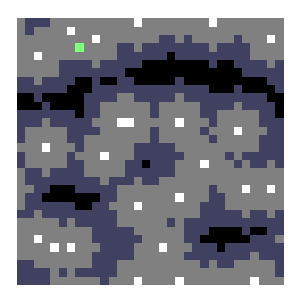
\includegraphics{00_000_grid.eps}
}
\caption["`Leeres Szenario"' ohne Hindernisse]{"`Leeres Szenario"' ohne Hindernisse}
\label{empty_grid:fig}
\end{figure}

\subsection{Szenario mit zuf�llig verteilten Hindernissen}\label{random_scenario_definition:sec}

Zwei Parameter bestimmen das Aussehen des Szenarios mit zuf�llig verteilten Hindernissen, zum einen der Prozentsatz an Hindernissen an der Gesamtzahl der Felder des Torus (Hindernissanteil~\(\lambda_{h}\)), zum anderen der Grad inwieweit die Hindernisse zusammenh�ngen (Verkn�pfungsfaktor~\(\lambda_{p}\)).\\
Bei der Erstellung des Szenarios bestimmt \(\lambda_{p}\) die Wahrscheinlichkeit f�r jedes einzelne angrenzende freie Feld, dass beim Verteilen der Hindernisse nach dem Setzen eines Hindernisses dort sofort ein weiteres Hindernis gesetzt wird. \(\lambda_{p} = 0.0\) erg�be somit eine v�llig zuf�llig verteilte Menge an Hindernissen, w�hrend ein Wert von \(1.0\) eine oder mehrere stark zusammenh�ngende Strukturen schafft. Wird der Prozentsatz an Hindernissen \(\lambda_{h}\) auf \(0.0\) gesetzt, dann entspricht diesem dem oben erw�hnten leeren Szenario. Ein Wert von \(1.0\) w�rde eine v�llige Abdeckung des Torus bedeuten und w�re f�r einen Test somit unbrauchbar. Hier sollen nur geringe Werte bis \(0.4\) betrachtet werden, wobei sp�ter in Tests sich auf Werte bis \(0.2\) beschr�nkt wird, da bei gro�en Hindernissanteil die lokalen Entscheidungen einzelner Agenten zu wichtig werden, da das Zielobjekt sich oft nur in einem kleinen Bereich aufh�lt TODO

In Abbildung~(\ref{random_grid_005:fig}), Abbildung~(\ref{random_grid_01:fig}), Abbildung~(\ref{random_grid_02:fig}) und Abbildung~(\ref{random_grid_04:fig}) werden Beispiele f�r zuf�llige Szenarien gegeben mit \(\lambda_{h} = 0.05\), \(0.1\), \(0.2\) bzw. \(0.4\) und \(\lambda_{p} = 0.01\), \(0.5\) bzw. \(0.99\).

\begin{figure}[htbp]
\centerline{	
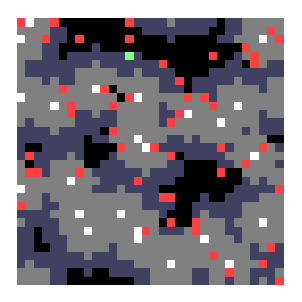
\includegraphics{005_001_grid.eps}
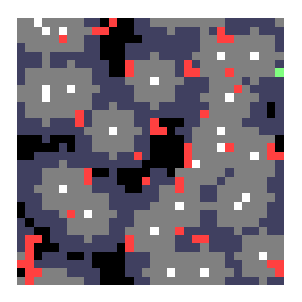
\includegraphics{005_050_grid.eps}
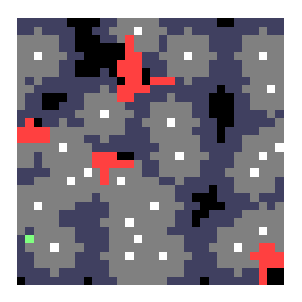
\includegraphics{005_099_grid.eps}
}
\caption[Szenario mit zuf�llig verteilten Hindernissen mit $\lambda_{h} = 0.05$] {Szenario mit zuf�llig verteilten Hindernissen mit Hindernissanteil \(\lambda_{h} = 0.05\) und Verkn�pfungsfaktor \(\lambda_{p} = 0.01\), \(0.5\) bzw. \(0.99\).}
\label{random_grid_005:fig}
\end{figure}

\begin{figure}[htbp]
\centerline{	
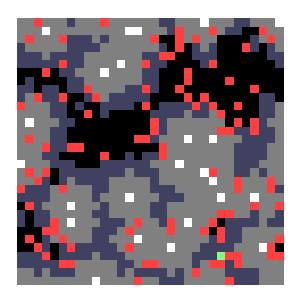
\includegraphics{01_001_grid.eps}
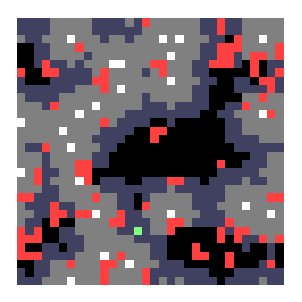
\includegraphics{01_050_grid.eps}
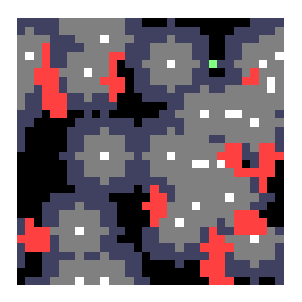
\includegraphics{01_099_grid.eps}
}
\caption[Szenario mit zuf�llig verteilten Hindernissen mit $\lambda_{h} = 0.1$] {Szenario mit zuf�llig verteilten Hindernissen mit Hindernissanteil \(\lambda_{h} = 0.1\) und Verkn�pfungsfaktor \(\lambda_{p} = 0.01\), \(0.5\) bzw. \(0.99\).}
\label{random_grid_01:fig}
\end{figure}

\begin{figure}[htbp]
\centerline{	
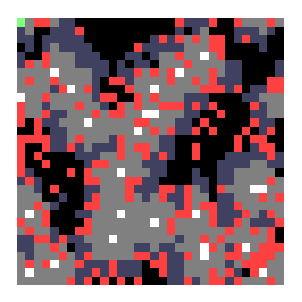
\includegraphics{02_001_grid.eps}
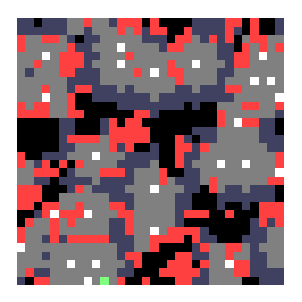
\includegraphics{02_050_grid.eps}
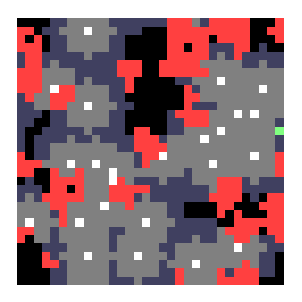
\includegraphics{02_099_grid.eps}
}
\caption[Szenario mit zuf�llig verteilten Hindernissen mit $\lambda_{h} = 0.2$] {Szenario mit zuf�llig verteilten Hindernissen mit Hindernissanteil \(\lambda_{h} = 0.2\) und Verkn�pfungsfaktor \(\lambda_{p} = 0.01\), \(0.5\) bzw. \(0.99\).}
\label{random_grid_02:fig}
\end{figure}

\begin{figure}[htbp]
\centerline{	
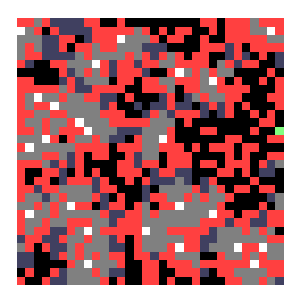
\includegraphics{04_001_grid.eps}
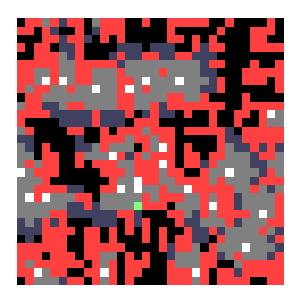
\includegraphics{04_050_grid.eps}
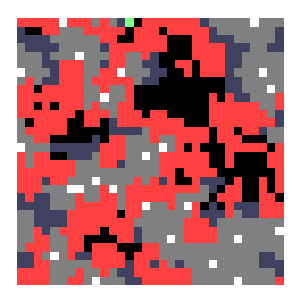
\includegraphics{04_099_grid.eps}
}
\caption[Szenario mit zuf�llig verteilten Hindernissen mit $\lambda_{h} = 0.4$] {Szenario mit zuf�llig verteilten Hindernissen mit Hindernissanteil \(\lambda_{h} = 0.4\) und Verkn�pfungsfaktor \(\lambda_{p} = 0.01\), \(0.5\) bzw. \(0.99\).}
\label{random_grid_04:fig}
\end{figure}


\subsection{S�ulen Szenario}

In diesem Szenario werden regelm��ig, mit jeweils 7 Feldern Zwischenraum zueinander,  Hindernisse auf dem Torus verteilt. Idee ist, dass die Agenten eine kleine Orientierungshilfe besitzen sollen, aber gleichzeitig m�glichst wenig Hindernisse verteilt werden. Das Zielobjekt startet an zuf�lliger Position, die Agenten starten mit m�glichst gro�em Abstand zum Zielobjekt. Abbildung~\ref{pillar_grid:fig} zeigt ein Beispiel f�r den Startzustand eines solchen Szenarios, bei der das Zielobjekt sich in der Mitte und die Agenten am Rand befinden.

\begin{figure}[htbp]
\centerline{	
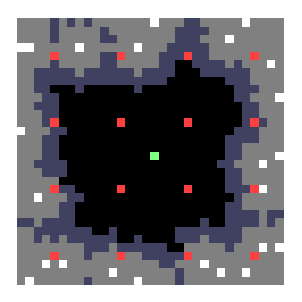
\includegraphics{pillar_grid.eps}
}
\caption[Startzustand des S�ulen Szenarios]{Startzustand des S�ulen Szenarios mit regelm��ig angeordneten Hindernissen und zuf�lliger Verteilung von Agenten mit m�glichst gro�em Abstand zum Zielobjekt}
\label{pillar_grid:fig}
\end{figure}



\subsection{Schwieriges Szenario}\label{difficult_scenario:sec}

Hier wird der Torus an der rechten Seite vollst�ndig durch Hindernisse blockiert, um den Torus zu halbieren. Alle Agenten starten (zuf�llig verteilt) am linken Rand, der Zielagent startet auf der rechten Seite.\\
In regelm��igen Abst�nden (7 Felder Zwischenraum) befindet sich eine vertikale Reihe von Hindernissen mit �ffnungen von 4 Feldern Breite abwechselnd im oberen Viertel und dem unteren Viertel.\\
Idee dieses Szenarios ist es, zu testen, inwieweit die Agenten durch die �ffnungen zum Ziel finden k�nnen. Ohne Orientierung an den �ffnungen und anderen Agenten ist es sehr schwierig, sich durch das Szenario zu bewegen. Die sp�ter besprochenen Tests in Kapitel~\ref{test_schwieriges_szenario:sec} werden zeigen, dass dieses Szenario besonders schwierig f�r sich zuf�llig bewegende Agenten und Agenten mit einfacher Heuristik ist. Sp�ter in Kapitel~\

Abbildung~\ref{difficult_grid:fig} zeigt die Startkonfiguration des Szenarios.

\begin{figure}[htbp]
\centerline{	

\includegraphics{difficult_grid.eps}
}
\caption[Schwieriges Szenario]{Schwieriges Szenario mit fester, wallartiger Verteilung von Hindernissen in regelm��igen Abst�nden und mit �ffnungen, mit den Agenten mit zuf�lligem Startpunkt am linken Rand und mit dem Zielobjekt mit festem Startpunkt rechts oben}
\label{difficult_grid:fig}
\end{figure}



\section{Bestimmung der Qualit�t eines Algorithmus}\label{qualitaet:sec}

Die Qualit�t eines Algorithmus zu einem Problem wird anhand des Anteils der Zeit berechnet, die er das Zielobjekt w�hrend des Problems �berwachen (d.h. das Zielobjekt innerhalb einer Distanz von h�chstens \emph{reward range} halten) konnte, relativ zur Gesamtzeit.\\
Die Qualit�t eines Algorithmus zu einer Anzahl von Problemen (also einem Experiment) wird Anhand des Gesamtanteil der Zeit berechnet, die er das Zielobjekt w�hrend aller Probleme �berwachen konnte, relativ zur Gesamtzeit aller Probleme.\\
Die Qualit�t eines Algorithmus entspricht dem Durchschnitt der Qualit�ten des Algorithmus mehrerer Experimente.\\
Die Halbzeitqualit�t eines Algorithmus zu einem Problem entspricht dem Anteil der Zeit, die der Algorithmus das Zielobjekt w�hrend jeweils der zweiten H�lfte des Problems �berwachen konnte, relativ zur halben Gesamtzeit.\\
Die Halbzeitqualit�t eines Algorithmus zu einer Anzahl von Problemen entspricht dem Anteil der Zeit, die der Algorithmus das Zielobjekt w�hrend jeweils der zweiten H�lfte des Problems �berwachen konnte, relativ zur halben Gesamtzeit aller Probleme.\\
Die Halbzeitqualit�t eines Algorithmus entspricht dem Durchschnitt aller Halbzeitqualit�ten des Algorithmus mehrerer Experimente.\\
Ein Vergleich der Qualit�t mit der Halbzeitqualit�t eines Algorithmus erm�glicht einen Einblick, wie gut sich der Algorithmus verh�lt, nachdem er sich auf das Problem bereits eine Zeit lang einstellen konnte.\\

\chapter{Agenten}

\section{Sensoren}\label{sensoren:sec}

Jeder Agent besitzt 3 Gruppen mit jeweils 8 Sensoren. Alle Sensoren sind visuelle, bin�re Sensoren mit begrenzter Reichweite und k�nnen nur feststellen, ob sich in ihrem Sichtbereich ein entsprechendes Objekt befindet oder nicht. Andere Objekte blockieren die Sicht, Sichtlinien werden durch einen einfachen Bresenham-Algorithmus bestimmt.\\
Jede Gruppe von Sensoren nimmt einen anderen Typ von Objekt wahr. Die erste Gruppe nimmt das Zielobjekt, die zweite Gruppe andere Agenten und die dritte Gruppe Hindernisse wahr.\\
Sensoren sind jeweils bestimmte Richtungen ausgerichtet (Norden, Osten, S�den und Westen, wobei auf den Abbildungen in dieser Arbeit Norden immer oben ist) und wird auf ``wahr'' (\(1\)) gesetzt, wenn sich in dem Sichtbereich des Sensors ein entsprechendes Objekt befindet.\\
Die 8 Sensoren in einer Gruppe sind in 4 Richtungen mit jeweils einem Sensorenpaar aufgeteilt. Ein Sensorenpaar besteht aus zwei Sensoren mit unterschiedlich gro�er Sichtweite, mit der der Agent also rudiment�r die Entfernung zu anderen Objekten feststellen kann. 

\[
\underbrace{z_{s_{N}} z_{r_{N}} z_{s_{O}} z_{r_{O}} z_{s_{S}} z_{r_{S}} z_{s_{W}} z_{r_{W}}}_{Erste~Gruppe~(Zielobjekt)}
\underbrace{a_{s_{N}} a_{r_{N}} a_{s_{O}} a_{r_{O}} a_{s_{S}} a_{r_{S}} a_{s_{W}} a_{r_{W}}}_{Zweite~Gruppe~(Agenten)}
\underbrace{h_{s_{N}} h_{r_{N}} h_{s_{O}} h_{r_{O}} h_{s_{S}} h_{r_{S}} h_{s_{W}} h_{r_{W}}}_{Dritte~Gruppe~(Hindernisse)}
\]

TODO darauf Bezug nehmen

\begin{verbatim}
TODO Beispiele f�r Sensoren
a) 10 00 00 00 . 00 00 00 00 . 00 00 00 00
b) 00 00 00 00 . 00 00 00 00 . 00 00 00 00
c) 00 00 00 00 . 11 00 10 00 . 00 00 00 00
d) 00 00 00 00 . 00 00 00 00 . 00 00 00 00
e) 00 00 00 00 . 00 00 00 00 . 00 00 00 00
\end{verbatim}



Die Sichtweite des ersten Sensors eines Paares wird �ber den Parameter \emph{sight range} bestimmt, die Sichtweite des zweiten Sensors �ber den Parameter \emph{reward range} (siehe auch Kapitel~\ref{sichtbarket:sec}). Allgemein soll \emph{sight range = 5.0} und \emph{reward range = 2.0} betragen, der �berwachte Bereich ist also eine Teilmenge des sichtbaren Bereichs. Anzumerken sei hier, dass deshalb ein Sensorenpaar (0\/1) nicht auftreten kann.\\
Sei \(r(O1, O2)\) die Distanz zwischen dem Objekt, das die Sensordaten erfasst und dem n�chstliegenden Objekt des Typs, den der Sensor wahrnehmen kann, dann gibt es folgende F�lle:

\begin{enumerate}
\item (0/0) : \(r(O_1, O_2) > \) \emph{sight range} (kein passendes Objekt in Sichtweite)
\item (1/0) : \emph{reward range} \( < r(O_1, O_2) \le \) \emph{sight range} (Objekt in Sichtweite)
\item (1/1) : \(r(O_1, O_2) \le \) \emph{reward range} (Objekt in Sicht- und �berwachungsreichweite)
\item (0/1) : \emph{reward range} \(\ge r(O_1, O_2) > \) \emph{sight range} (Fall kann nicht auftreten, da \emph{reward range} \( < \) \emph{sight range})
\end{enumerate}

In Abbildung ~\ref{sight_directions:fig} sind alle Sichtkegel (dunkler und heller Bereich) und �berwachungsreichweiten (heller Bereich) f�r die einzelnen Richtungen dargestellt. 

TODO von 3-5 auf 2-5 um�ndern

\begin{figure}[htbp]
\centerline{	
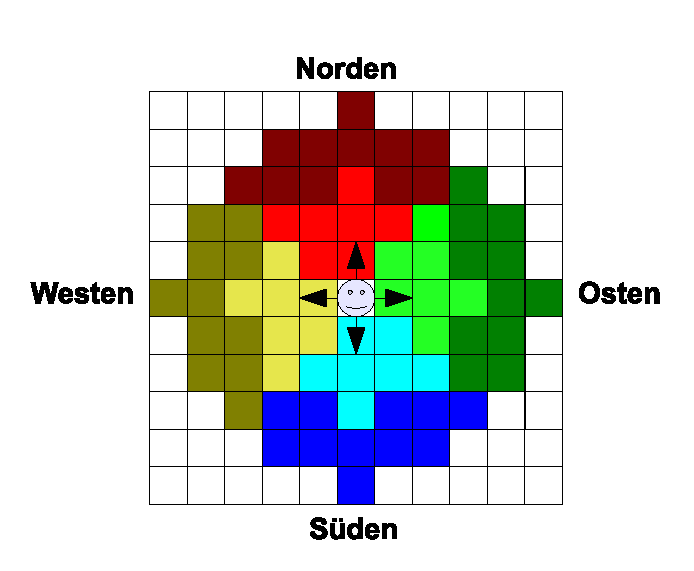
\includegraphics{sight_directions.eps}
}
\caption[Sicht- und �berwachungsreichweite eines Agenten]{Sicht- (2.0) und �berwachungsreichweite (5.0) eines Agenten, jeweils f�r die einzelnen Richtungen}
\label{sight_directions:fig}
\end{figure}

\section{F�higkeiten}\label{agent_abilities:sec}

Jeder Agent kann in jedem Schritt zwischen vier verschiedenen Aktionen w�hlen, die den vier Richtungen (Norden, Osten, S�den, Westen), bei der der Agent sich nicht bewegt, entsprechen. Agenten k�nnen pro Zeiteinheit genau einen Schritt durchf�hren. Das Zielobjekt kann je nach Szenarioparameter mehrere Schritte ausf�hren.

\section{Ablauf der Bewegung}
Alle Agenten werden nacheinander in der Art abgearbeitet, dass der jeweilige Agent die aktuellen Sensordaten aus der Umgebung holt und anhand dieser die n�chste Aktion bestimmt. Ung�ltige Aktionen, d.h. der Versuch sich auf ein besetztes Feld zu bewegen, schlagen fehl und der Agent f�hrt in diesem Schritt keine Aktion aus, wird aber nicht weiter bestraft. Eine detaillierte Beschreibung der Bewegung im Kontext anderer Agenten und Programmteile wird in Kapitel~\ref{reihenfolge:sec} gegeben.

\section{Grunds�tzliche Algorithmen der Agenten}

Neben denjenigen Algorithmen, die auf LCS basieren und in Kapitel~\ref{lcs:cha} besprochen werden, gibt es folgende Grundtypen, die dazu dienen, die Qualit�t der anderen Algorithmen einzuordnen. Wesentliches Merkmal im Vergleich zu auf LCS basierenden Algorithmen ist, dass sie statische, handgeschriebene Regeln benutzen und den Erfolg oder Misserfolg ihrer Aktionen ignorieren, d.h. ihre Regeln nicht anpassen.

\subsection{``Zuf�lliger Algorithmus''}\label{randomized_movement:sec}
Bei diesem Algorithmus wird in jedem Schritt wird eine zuf�llige Aktion ausgef�hrt. Abbildung ~(\ref{agent_random:fig}) zeigt eine Beispielsituation bei der der Agent jegliche Sensordaten ignoriert und eine Aktion zuf�llig ausw�hlen wird.

\begin{figure}[htbp]
\centerline{	
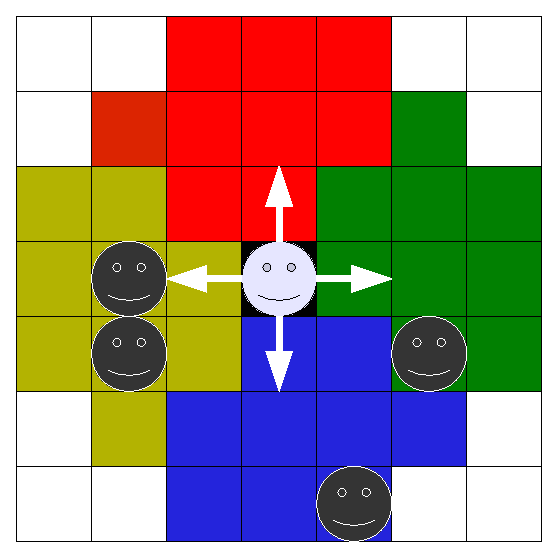
\includegraphics{agent_random.eps}
}
\caption[Sich zuf�llig bewegender Agent]{Agent bewegt sich in eine zuf�llige Richtung (oder bleibt stehen)}
\label{agent_random:fig}
\end{figure}

\subsection{Einfache Heuristik}\label{simple_heuristik:sec}
Ist das Zielobjekt in Sichtweite, bewegt sich ein Agent mit dieser Heuristik  auf das Zielobjekt zu, ist es nicht in Sichtweite, f�hrt er eine zuf�llige Aktion aus. Abbildung ~(\ref{simple_agent_to_goal:fig}) zeigt eine Beispielsituation bei der sich das Zielobjekt (Stern) im S�den befindet, der Agent mit einfacher Heuristik die anderen Agenten ignoriert und sich auf das Ziel zubewegen m�chte. 

\begin{figure}[htbp]
\centerline{	
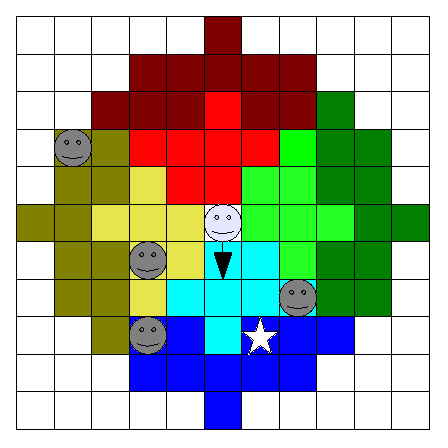
\includegraphics{simple_agent_to_goal.eps}
}
\caption[Agent mit einfacher Heuristik]{Agent mit einfacher Heuristik: Sofern es sichtbar ist bewegt sich der Agent auf das Zielobjekt zu.}
\label{simple_agent_to_goal:fig}
\end{figure}

\subsection{Intelligente Heuristik}\label{intelligent_heuristik:sec}
Ist der Zielobjekt in Sicht, verh�lt sich diese Heuristik wie die einfache Heuristik. Ist das Zielobjekt dagegen nicht in Sicht, wird versucht, anderen Agenten auszuweichen, um ein m�glichst breit gestreutes Netz aus Agenten aufzubauen. In der Implementation hei�t das, dass unter allen Richtungen, in denen kein anderer Agent gesichtet wurde, eine Richtung zuf�llig ausgew�hlt wird und falls alle Richtungen belegt (oder alle frei) sind, wird aus allen Richtungen eine zuf�llig ausgew�hlt wird. In Abbildung~(\ref{intelligent_agent:fig}) sieht der Agent das Zielobjekt nicht und w�hlt deswegen eine Richtung, in der die Sensoren keine Agenten anzeigt, in diesem Fall Norden.

\begin{figure}[htbp]
\centerline{	
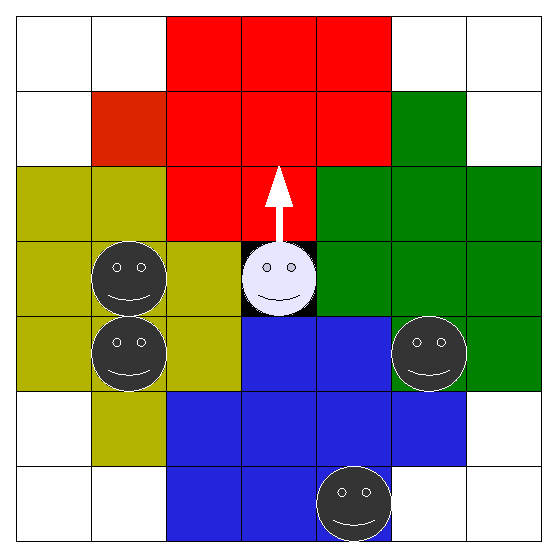
\includegraphics{intelligent_agent.eps}
}
\caption[Agent mit intelligenter Heuristik]{Agent mit intelligenter Heuristik: Falls das Zielobjekt nicht sichtbar ist bewegt sich der Agent von anderen Agenten weg.}
\label{intelligent_agent:fig}
\end{figure}

\chapter{Das Zielobjekt}


Die Typen von Zielobjekten werden zum einen �ber ihre Geschwindigkeit und zum anderen �ber ihre Bewegungsart definiert. Neben der Gr��e des Torus und den Hindernissen tr�gt der Typ des Zielobjekts wesentlich zur Schwierigkeit eines Szenarios bei, da dieser die Aufenthaltswahrscheinlichkeiten des Zielobjekts unter Einbeziehung des Zustands des letzten Zeitschritts bestimmt. Die Schwierigkeit bestimmt sich �ber die Summe der erwarteten Aufenthaltswahrscheinlichkeiten in nicht �berwachten Feldern geteilt durch die Summe der Aufenthaltswahrscheinlichkeiten in �berwachten Feldern.

\section{Basiseigenschaften}

Im wesentlichen entspricht ein Zielobjekt einem Agenten, d.h. das Zielobjekt kann sich bewegen und besitzt Sensoren. 

Gemeinsam haben alle Arten von Bewegungen des Zielobjekts, dass, wenn dem Algorithmus kein freies Feld zur Verf�gung steht, ein zuf�lliges, freies Feld in der N�he ausgew�hlt und dort hingesprungen wird. Dies kommt einem Neustart gleich und ist notwendig um eine Verf�lschung des Ergebnisses zu verhindern, das daher r�hren kann, dass ein oder mehrere Agenten (zusammen mit eventuellen Hindernissen) alle vier Bewegungsrichtungen des Zielobjekts blockieren.\\
Andererseits ist auch der Sprung eine Verf�lschung, falls bei einem Durchlauf eine ganze Anzahl von Spr�ngen durchgef�hrt worden sein, sollte man deshalb das Ergebnis verwerfen und andere Random-Seed Werte benutzen.

TODO wie oft das aufgetreten ist

TODO benachbarte Hindernisse aus Bewegung ausschliessen, N�hesensor

\section{Typen von Zielobjekten}

\subsection{Typ ``Total Random''}
Ein Zielobjekt dieses Typs springt zu einem zuf�lligen (freien) Feld auf dem Torus. Mit dieser Einstellung kann die Abdeckung des Algorithmus gepr�ft werden, d.h. inwieweit die Agenten jeweils au�erhalb der �berwachungsreichweite anderer Agenten bleiben. Jegliche Anpassung an die Bewegung des Zielobjekts ist hier wenig hilfreich, ein Agent kann nicht einmal davon ausgehen, dass sich das Zielobjekt in der N�he seiner Position der letzten Zeiteinheit befindet. Die Aufenthaltswahrscheinlichkeit f�r jedes freie Feld ist hierbei \(\frac{1}{n}\), wobei \(n\) die Anzahl der freien Felder entspricht.

\subsection{``Random Movement''}
Wie ``Random Movement'' bei Agenten (~\ref{randomized_movement:sec}). Sind alle m�glichen Felder belegt, wird wie oben beschrieben auf ein zuf�lliges Feld gesprungen. Diesen Fall au�en vorgelassen betr�gt die Aufenthaltswahrscheinlichkeit f�r die 4 angrenzenden Felder jeweils \(\frac{1}{5}\) und das Zielobjekt bleibt mit Wahrscheinlichkeit \(\frac{1}{5}\) stehen.

\subsection{``One direction change''}
Mit dieser Einstellung wird die der letzten Richtung entgegengesetzten Richtung aus der Menge der Auswahlm�glichkeiten entfernt und von den verbleibenden drei Richtungen (plus der Aktion ``Stehenbleiben'') eine zuf�llig ausgew�hlt. Sind alle drei Richtungen versperrt, wird stehengeblieben.\\
War die letzte Aktion nicht eine Bewegungsrichtung, sondern die Aktion ``Stehenbleiben'', so wird eine zuf�llige Richtung ausgew�hlt. Sind alle Richtungen versperrt, wird auch hier wieder auf ein zuf�lliges Feld gesprungen.
Die Aufenthaltswahrscheinlichkeit betr�gt im Fall ohne angrenzende Hindernisse f�r die Felder vor, links und rechts (relativ zur Bewegungsrichtung im vergangenen Zeitschritt) also \(\frac{1}{3}\). In Abbildung~\ref{goal_agent_one_direction_change:fig} ist eine Beispielsituation zu sehen, bei der der Zielagent sich zuletzt nach Norden bewegt hat und nun zwischen Norden, Westen und Osten ausw�hlen kann.

\begin{figure}[htbp]
\centerline{	
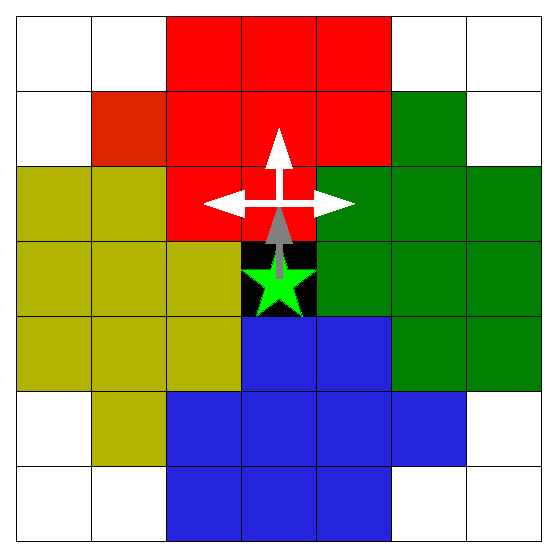
\includegraphics{goal_direction_change.eps}
}
\caption[Zielobjekt mit maximal einer Richtungs�nderung]{Zielobjekt macht pro Schritt maximal eine Richtungs�nderung}
\label{goal_agent_one_direction_change:fig}
\end{figure}

\subsection{``Always same direction''}
Der Zielobjekt versucht, immer Richtung Norden zu gehen. Ist das Zielfeld blockiert, w�hlt er ein zuf�lliges, angrenzendes, freies Feld im Westen oder Osten. Anzumerken ist, dass dies zus�tzliche F�higkeiten darstellen, d.h. das Zielobjekt kann feststellen, ob sich direkt angrenzend ein Hindernis im Norden befindet, w�hrend normale Agenten, was die Distanz betrifft, keine Informationen dar�ber besitzen k�nnen.\\
Sind auch die Felder im Westen und Osten belegt, springt er auf ein zuf�lliges freies Feld. Schafft es der Zielobjekt innerhalb von einer bestimmten Zahl (Breite des Spielfelds) von Schritten nicht, einen weiteren Schritt nach Norden zu gehen, wird ebenfalls gesprungen, um ein ``Festh�ngen'' an einem Hindernis zu vermeiden. Ohne Hindernisse ergibt sich also eine Aufenthaltswahscheinlichkeit von \(1.0\) im dar�berliegenden Feld im Norden. In Abbildung~\ref{goal_agent_always_same_direction:fig} sind drei Situationen dargestellt, zum einen ein wiederholtes hin- und herlaufen unter den Hindernissen, der Weg links um die Hindernisse herum und der Weg rechts um die Hindernisse herum.

TODO im Bild den Pfeil nach rechts bzw. links raus, wo er bereits im Norden frei ist

\begin{figure}[htbp]
\centerline{	
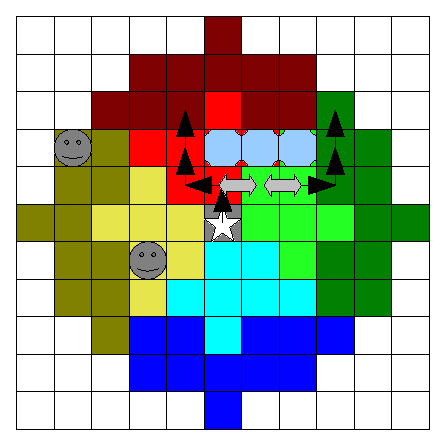
\includegraphics{goal_always_same_direction.eps}
}
\caption[Zielobjekt das sich, wenn m�glich, immer nach Norden bewegt]{Zielobjekt bewegt sich, wenn m�glich, immer nach Norden}
\label{goal_agent_always_same_direction:fig}
\end{figure}

\subsection{``Intelligent (Open)''}
Das Zielobjekt versucht bei der Auswahl der Aktion m�glichst die Aktion zu w�hlen, bei der es au�erhalb der Sichtweite der Agenten bleibt, es werden also alle Richtungen gestrichen, in denen ein anderer Agent gesichtet wird. Von den verbleibenden Richtungen werden au�erdem mit 20\% Wahrscheinlichkeit alle Richtungen gestrichen, in denen sich ein Hindernis befindet. Sind alle Richtungen gestrichen worden, bewegt sich das Zielobjekt zuf�llig. Sind alle Richtungen blockiert, springt es wie in den anderen Varianten auch auf ein zuf�lliges Feld. In Abbildung~\ref{goal_agent_intelligent_open:fig} wird die Richtung Westen gestrichen, da sich dort ein Agent befindet. Im Norden und Osten befinden sich Hindernisse, diese Richtungen werden jeweils mit 20\% gestrichen, w�hrend die Richtung S�den mit Sicherheit als Auswahlm�glichkeit �brig bleibt. Die Aufenthaltswahrscheinlichkeit f�r Norden und Osten w�ren also jeweils \(\frac{8*8}{3*10*10}+\frac{2*8}{2*10*10} = \frac{88}{300}\) und \(\frac{8*8}{3*10*10}+\frac{2*2*8}{2*10*10}+\frac{2*2}{10*10}=\frac{124}{300}\) f�r den S�den.

\begin{figure}[htbp]
\centerline{	
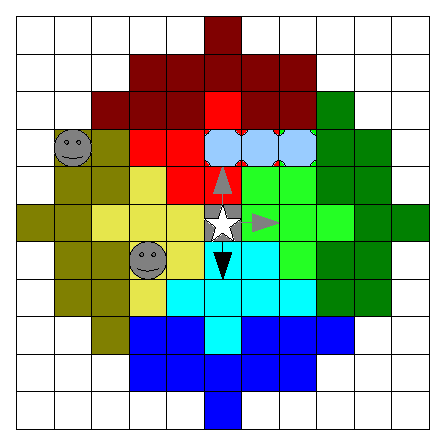
\includegraphics{goal_intelligent_open.eps}
}
\caption[Sich intelligent verhaltendes Zielobjekt der Agenten und Hindernissen ausweicht]{Zielobjekt bewegt sich mit bestimmter Wahrscheinlichkeit von Agenten und gr��erer Wahrscheinlichkeit von Hindernissen weg}
\label{goal_agent_intelligent_open:fig}
\end{figure}

\subsection{``Intelligent (Hide)''}
Das Zielobjekt vermeidet Agenten wie bei ``Intelligent (Open)'', streicht aber statt Richtungen mit Hindernissen Richtungen ohne Hindernisse mit 20\% Wahrscheinlichkeit, tendiert also eher dazu, auf Hindernisse zuzugehen. Idee ist, dass es sich dadurch m�glicherweise den Blicken der Agenten entziehen kann. Betrachten wir in Abbildung~\ref{goal_agent_intelligent_hide:fig} die selbe Situation wie bei ``Intelligent (Open)'' so sind die Aufenthaltswahrscheinlichkeiten von Norden und Osten mit denen von S�den vertauscht.

\begin{figure}[htbp]
\centerline{	
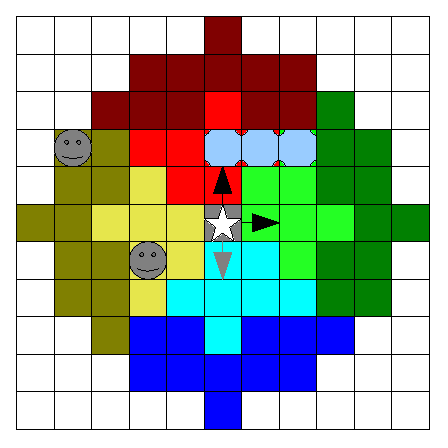
\includegraphics{goal_intelligent_hide.eps}
}
\caption[Sich intelligent verhaltendes Zielobjekt der Agenten ausweicht und Hindernisse sucht]{Zielobjekt bewegt sich von Agenten weg und mit bestimmter Wahrscheinlichkeit auf Hindernisse zu}
\label{goal_agent_intelligent_hide:fig}
\end{figure}

\subsection{``LCS''}
Eine LCS Implementierung, die der Implementierung eines LCS Agenten entspricht. Das Ziel des Zielobjekts ist es hier aber, es zu vermeiden, Agenten zu �berwachen (bzw. umgekehrt eine �berwachung durch andere Agenten zu vermeiden). Eine genaue Beschreibung folgt im Kapitel~\ref{lcs:cha} und soll hier nur der Vollst�ndigkeit halber erw�hnt werden.

TODO auch ein eigenes goal agent lcs kapitel machen
TODO Pendelbewegung?
TODO Fester Pfad?

\chapter{Ablauf der Simulation}\

\section{Hauptschleife}

In der Hauptschleife (siehe Programm~\ref{mainExperiment:pro}) wird ein Experiment mit vorgegebener Konfiguration (``\emph{Configuration}'') durchgef�hrt. Dabei werden eine Anzahl von Problemen abgearbeitet, bei denen jeweils der Torus auf den Startzustand gesetzt, das eigentliche Problem berechnet und ein neuer \emph{random seed} Wert gesetzt wird.


\newlisting{Zentrale Schleife f�r einzelne Experimente}{mainExperiment:pro}
/**
 * F�hrt eine Anzahl von Problemen aus
 * @param experiment_nr Nummer des auszuf�hrenden Experiments
 */
  public void doOneMultiStepExperiment(int experiment_nr) {
    int currentTimestep = 0;

  /**
   * number of problems for the same population
   */
    for (int i = 0; i < Configuration.getNumberOfProblems(); i++) {

    /**
     * Erstellt einen neuen Torus und verteilt Agenten und das Zielobjekt neu
     */
      BaseAgent.grid.resetState();

    /**
     * F�hre Problem aus und aktualisiere aktuellen Zeitschritt
     */
      currentTimestep = doOneMultiStepProblem(currentTimestep);

    /**
     * Initialisiere neuen "Random Seed" Wert
     */
      Misc.initSeed(Configuration.getRandomSeed() + 
        experiment_nr * Configuration.getNumberOfProblems() + 1 + i);
    }
  }
\end{lstlisting}


\section{Reihenfolge der Ausf�hrung (\emph{doOneMultiStepProblem()})}\label{reihenfolge:sec}

TODO vielleicht erst noch eine allgemeine �bersicht geben

F�r die Berechnung eines einzelnen Problems (``\emph{doOneMultiStepProblem()}'') stellt sich die Frage nach der Genauigkeit und der Reihenfolge der Abarbeitung, da die Simulation nicht parallel, sondern schrittweise auf einem diskreten Torus abl�uft. Dies kann u.U. dazu f�hren, dass je nach Position in der Liste abzuarbeitender Agenten die Informationen �ber die Umgebung unterschiedlich alt sind. Die Frage ist deshalb, in welcher Reihenfolge Sensordaten ermittelt, ausgewertet, Agenten bewegt, intern sich selbst bewertet und global die Qualit�t gemessen wird.\\
Da eine Aktion auf Basis der Sensordaten ausgew�hlt wird, ist die erste Restriktion, dass eine Aktion nach der Verarbeitung der Sensordaten stattfinden muss. Und da Aktionen bewertet werden sollen, also jeweils der Zustand nach der Bewegung mit dem gew�nschten Zustand verglichen werden soll, ist die zweite Restriktion, dass die Bewertung einer Aktion nach dessen Ausf�hrung stattfinden muss.\\
Ansonsten ergeben sich folgende M�glichkeiten:

\begin{enumerate}
\item F�r alle Agenten werden erst einmal die neuen Sensordaten erfasst und sich f�r eine Aktion entschieden. Sind alle Agenten abgearbeitet, werden die Aktionen ausgef�hrt.
\item Die Agenten werden nacheinander abgearbeitet, es werden jeweils neue Sensordaten erfasst und sich sofort f�r eine neue Aktion entschieden. 
\end{enumerate}

Bei der ersten M�glichkeit haben alle Agenten die Sensordaten vom Beginn der Zeiteinheit, w�hrend bei der zweiten M�glichkeit sp�ter verarbeitete Agenten bereits die Aktionen der bereits berechneten Agenten miteinbeziehen k�nnen. Umgekehrt k�nnen dann fr�here Agenten bessere Positionen fr�her besetzen. Da aufgrund der primitiven Sensoren nicht davon auszugehen ist, dass Agenten beginnende Bewegungen (und somit deren jeweilige Zielposition) anderer Agenten einbeziehen k�nnen, soll jeder Agent von den Sensorinformationen zu Beginn der Zeiteinheit ausgehen.\\
Wenn sich mehrere Agenten auf dasselbe Feld bewegen wollen, dann spielt die Reihenfolge der Ausf�hrung der Aktionen eine Rolle. Wird die Liste der Agenten einfach linear abgearbeitet, k�nnen Agenten mit niedriger Position in der Liste die Aktion auf Basis j�ngerer Sensordaten f�llen. Dies kann dazu f�hren, dass Aktionen von Agenten mit h�herer Position in der Liste eher fehlschlagen, da das als frei angenommene Feld nun bereits besetzt ist. Da es keinen Grund gibt, Agenten mit niedrigerer Position zu bevorteilen, werden die Aktionen der Agenten in zuf�lliger Reihenfolge abgearbeitet.\\
Bez�glich der Bewegung ergibt sich hierbei eine weitere Frage, n�mlich wie unterschiedliche Bewegungsgeschwindigkeiten behandelt werden sollen, da alle Agenten eine Einheitsgeschwindigkeit von maximal einem Feld pro Zeiteinheit haben, w�hrend sich das Zielobjekt je nach Szenario gleich eine ganze Anzahl von Feldern bewegen kann (siehe auch Kapitel~\ref{base_properties_goal:sec}).
Die Entscheidung fiel hier auf eine zuf�llige Verteilung. Kann sich das Zielobjekt um \(n\) Schritte bewegen, so wird seine Bewegung in \(n\) Einzelschritte unterteilt, die nacheinander mit zuf�lligen Abst�nden (d.h. Bewegungen anderer Agenten) ausgef�hrt werden.\\
Eine weitere Frage ist, wie das Zielobjekt diese weiteren Schritte festlegen soll. Hier soll ein Sonderfall eingef�hrt werden, sodass das Zielobjekt in einer Zeiteinheit mehrmals (\(n\)-mal) neue Sensordaten erfassen und sich f�r eine neue Aktion entscheiden kann.

\section{Messung der Qualit�t}\label{qualitaetsmessung:sec}

Eine konkrete Antwort kann man auf diese zwei Fragen nicht geben, sie h�ngt  davon ab, was man denn nun eigentlich erreichen m�chte, also auf welche Weise die Qualit�t des Algorithmus bewertet wird. Der naheliegendste Messzeitpunkt ist, nachdem sich alle Agenten bewegt haben. Da die Agenten und das Zielobjekt in einem Durchlauf gemeinsam nacheinander bewegt werden, stellt sich die Frage nicht, ob wom�glich vor der Bewegung des Zielobjekts die Qualit�t gemessen werden sollen. Eine Messung nach der Bewegung des Zielobjekts w�rde diesem erlauben, sich vor jeder Messung optimal zu positionieren, was in einer geringeren Qualit�t f�r den Algorithmus resultiert, da sich das Zielobjekt aus der �berwachungsreichweite anderer Agenten hinausbewegen kann. Letztlich ist es eine Frage der Problemstellung, denn eine Messung nach Bewegung des Zielobjekts bedeutet letztlich, dass ein Agent einen gerade aus seiner �berwachungsreichweite heraus laufenden Zielobjekts in diesem Schritt nicht mehr �berwachen kann.\\
Da ein wesentlicher Bestandteil die Kooperation (und somit die Abdeckung des Torus anstatt dem Verfolgen des Zielobjekts) sein soll, soll ein Bewertungskriterium sein, inwieweit der Einfluss des Zielobjekts minimiert werden soll. Auch findet, wenn man vom realistischen Fall ausgeht, die Bewegung des Zielobjekts gleichzeitig mit allen anderen Agenten statt. Die Qualit�t wird somit nach der Bewegung des Zielobjekts gemessen. Die �berlegung unterstreicht auch nochmal, dass es besser ist, das Zielobjekt insgesamt wie einen normalen (aber sich mehrmals bewegenden) Agenten zu behandeln.\\

\section{Reihenfolge der Ermittlung des \emph{base reward}}

Keine der bisher vorgestellten Varianten machen Gebrauch von einem sogenannten \emph{base reward}, d.h.  TODO

Schlie�lich bleibt die Frage danach, wann gepr�ft werden soll, ob das Zielobjekt in �berwachungsreichweite ist, und wann sich somit ein \emph{reward} ergeben soll. Wesentliche Punkte hierbei sind, dass der Algorithmus sich anhand der Sensordaten selbst bewertet und pro Zeitschritt die Sensordaten nur einmal erhoben werden. Letzteres folgt aus der Auslegung von XCS, der in der Standardimplementation darauf ausgelegt ist, dass der Reward jeweils genau einer Aktion zugeordnet ist. Daraus ergibt sich auch, dass der Reward von bin�rer Natur ist ("`Zielobjekt in �berwachungsreichweite"' oder "`Zielobjekt nicht in �berwachungsreichweite"'), weshalb Zwischenzust�nde f�r den Reward, der sich aus der mehrfachen Bewegung des Zielobjekts ergeben k�nnte, ausgeschlossen werden soll (z.B. "`War zwei von drei Schritten in der �berwachungsreichweite"' \(\Rightarrow \frac{2}{3}\) Reward). Insbesondere w�rde dies eine mehrfache Erhebung der Sensordaten erfordern.\\

TODO Rewarderhebung f�r normale Agenten irrelevant, evtl teilen und in XCS Kapitel

F�r den Reward ergeben sich somit folgende M�glichkeiten:

\begin{enumerate}
\item Ermittlung der einzelnen \emph{reward} Werte jeweils direkt nach der Ausf�hrung einer einzelnen Aktion
\item Ermittlung aller \emph{reward} Werte nach Ausf�hrung aller Aktionen der Agenten und des Zielobjekts
\end{enumerate}

Werden die \emph{reward} Werte sofort ermittelt (Punkt 1), dann bezieht sich der Wert auf die veralteten Sensordaten vor der Aktion, die Aktion selbst w�rde bei der Ermittlung des \emph{reward} Werts also ignoriert werden. Bei Punkt 2 m�sste man bis zum neuen Zeitschritt warten, bis neue Sensordaten ermittelt wurden.


\section{Zusammenfassung}
Zusammenfassend sieht der Ablauf aller Agenten (inklusive des Zielobjekts) also wie folgt aus:

\begin{figure}[H]
\setbox0\vbox{\small
\begin{enumerate}
\item Bestimmen der aktuellen \textbf{Qualit�t}
\item Erfassung aller \textbf{Sensordaten}
\item Bestimmung der jeweiligen {\bfseries {\em reward} Werte} f�r die einzelnen Objekte f�r den letzten Schritt
\item \textbf{Wahl der Aktion} anhand der Regeln des jeweiligen Agenten
\item \textbf{Ausf�hrung der Aktion} (in zuf�lliger Reihenfolge, das Zielobjekt wiederholt Schritte 1 und 2 nach der Ausf�hrung der Aktion)
\end{enumerate}
}
\centerline{\fbox{\box0}}
\end{figure}

\section{Implementierung eines Problemablaufs}\label{implementierung_ablauf:sec}

In der Schleife der Funktion zur Berechnung eines Experiments (Programm~\ref{mainExperiment:pro}) wird die Funktion zur Berechnung des Problems (\emph{doOneMultiStepProblem()} in Programm~\ref{mainProblem:pro}) aufgerufen. Dort wird, in einer weiteren Schleife �ber die Anzahl der maximalen Schritte, die Sicht aktualisiert (\emph{updateSight()}), die Qualit�t bestimmt (\emph{updateStatistics()}), die neuen Sensordaten und die n�chste Aktion ermittelt (\emph{calculateAgents()}, siehe Programm~\ref{mainCalculate:pro}), der \emph{reward} Wert ermittelt (\emph{rewardAgents()}, siehe Programm~\ref{mainReward:pro}) und schlie�lich die Objekte bewegt (\emph{moveAgents()}, siehe Programm~\ref{mainMove:pro}). Die konkrete Umsetzung der dort aufgerufenen Funktionen (insbesondere \emph{calculateNextMove()} und \emph{calculateReward()}) wird im Kapitel~\ref{lcs_variants:cha} erl�utert (bzw. in Kapitel~\ref{agents:cha} was die Heuristiken betrifft, wobei \emph{calculateReward()} dort keine Rolle spielt und eine leere Funktion aufgerufen wird).


\newlisting{Zentrale Schleife f�r einzelne Probleme}{mainProblem:pro}
/**
 * F�hrt eine Anzahl von Schritten auf dem aktuellen Torus aus
 * @param stepCounter Aktuelle Zeitschritt
 * @return Der Zeitschritt nach der Ausf�hrung
 */
  private int doOneMultiStepProblem(int stepCounter) {
  /**
   * Zeitpunkt bis zu dem das Problem ausgef�hrt wird
   */
    int steps_next_problem = 
      Configuration.getNumberOfSteps() + stepCounter;    
    for (int currentTimestep = stepCounter; 
         currentTimestep < steps_next_problem; currentTimestep++) {

    /**
     * Ermittle die Sichtbarkeit und erhebe Statistiken
     */
      BaseAgent.grid.updateSight();
      BaseAgent.grid.updateStatistics(currentTimestep);

    /**
     * Ermittle neue Sensordaten und berechne Aktionen der Agenten
     */
      calculateAgents(currentTimestep);

    /**
     * Ermittle den Reward f�r alle Agenten (nach dem ersten Schritt)
     */
      if(currentTimestep > stepCounter) {
        rewardAgents(currentTimestep);
      }

    /**
     * F�hre zuvor berechnete Aktionen aus
     */
      moveAgents();
    }

    /**
     * Abschlie�ende Ermittlung des Rewards
     */
    BaseAgent.grid.updateSight();
    rewardAgents(steps_next_problem);
    return steps_next_problem;
  }
\end{lstlisting}



\newlisting{Zentrale Bearbeitung (Sensordaten und Berechnung der neuen Aktion) aller Agenten und des Zielobjekts innerhalb eines Problems}{mainCalculate:pro}
/**
 * Berechnet die Aktionen und f�hrt sie in zuf�lliger Reihenfolge aus
 * @param gaTimestep der aktuelle Zeitschritt
 */
  private void calculateAgents(final long gaTimestep) {

  /**
   * Ermittle Sensordaten und bestimme n�chste Bewegung
   */
    for(BaseAgent a : agentList) {
      a.aquireNewSensorData();
      a.calculateNextMove(gaTimestep);
    }
    BaseAgent.goalAgent.aquireNewSensorData();
    BaseAgent.goalAgent.calculateNextMove(gaTimestep);
  }
\end{lstlisting}



\newlisting{Zentrale Bearbeitung (Verteilung des Rewards) aller Agenten und des Zielobjekts innerhalb eines Problems}{mainReward:pro}
/**
 * Verteilt den Reward an alle Agenten
 */
  private void rewardAgents(final long gaTimestep) {
    for(BaseAgent a : agentList) {
      a.calculateReward(gaTimestep);
    }
    BaseAgent.goalAgent.calculateReward(gaTimestep);
  }
\end{lstlisting}



\newlisting{Zentrale Bearbeitung (Ausf�hrung der Bewegung) aller Agenten und des Zielobjekts innerhalb eines Problems}{mainMove:pro}
/**
 * F�hrt die berechnete Bewegungen der Agenten in zuf�lliger Reihenfolge aus
 */
  private void moveAgents(long gaTimestep) {
  /**
   * Erstelle Ausf�hrungsliste f�r alle Objekte (Zielobjekt mehrfach)
   */
    int goal_speed = Configuration.getGoalAgentMovementSpeed();
    ArrayList<BaseAgent> random_list = 
      new ArrayList<BaseAgent>(agentList.size() + goal_speed);

    random_list.addAll(agentList);
    for(int i = 0; i < goal_speed; i++) {
      random_list.add(BaseAgent.goalAgent);
    }

  /**
   * F�hre die ermittelten Aktionen in zuf�lliger Reihenfolge aus
   *   (Zielobjekt kann mehrfach ausgef�hrt werden).
   */
    int[] array = Misc.getRandomArray(random_list.size());
    for(int i = 0; i < array.length; i++) {
      BaseAgent a = random_list.get(array[i]);
      a.doNextMove();
      if(a.isGoalAgent() && goal_speed > 1) {
        goal_speed--;
        a.aquireNewSensorData();
        a.calculateNextMove(gaTimestep);
        a.calculateReward(gaTimestep);
      }
    }
  }
\end{lstlisting}


\chapter{Erste Analyse der Agenten ohne XCS}\label{analysis_sans_lcs:cha}

In diesem Kapitel sollen erste Analysen bez�glich der verwendeten Szenarien anhand des ``zuf�lligen Algorithmus''~\ref{randomized_movement:sec}, des Algorithmus mit ``einfacher Heuristik''~\ref{simple_heuristik:sec} und des Algorithmus mit ``intelligenter Heuristik''~\ref{intelligent_heuristik:sec} angefertigt werden. Die Ergebnisse aus der Analyse werden eine Grundlage f�r die vergleichende Betrachtung der Agenten mit XCS Algorithmen in Kapitel~\ref{lcs_analysis:cha} dienen, insbesondere werden sie Anhaltspunkte daf�r geben, welche Szenarien welche Eigenschaften der Algorithmen testen.

TODO: Ziel: Schwere Szenarien finden (schwierig f�r zuf�lligen, leicht f�r einfache heuristik)

\section{Statistische Merkmale}

Da keiner der hier vorgestellten Algorithmen lernt und somit statische Regeln besitzt, ist es nicht notwendig, die Qualit�ten der Algorithmen bei verschiedener Anzahl von Zeitschritten zu betrachten und zu vergleichen, die Zahl der Zeitschritte wird somit auf 500 festgesetzt. Au�erdem sollen in den Statistiken die Werte jeweils �ber einen Lauf von 10 Experimenten mit jeweils 10 Problemen ermittelt und gemittelt werden. Alle Werte sind auf 2 Stellen nach dem Komma gerundet. TODO

\subsection{Qualit�t}

\subsection{Abdeckung}

Die theoretisch maximal m�gliche Anzahl an Felder, die die Agenten innerhalb ihrer �berwachungsreichweite zu einem Zeitpunkt haben k�nnen, entspricht der Zahl der Agenten multipliziert mit der Zahl der Felder die ein Agent in seiner �bertragungsreichweite haben kann. Ist dieser Wert gr��er als die Gesamtzahl aller freien Felder, wird stattdessen dieser Wert benutzt.\\
Teilt man nun die Anzahl der momentan tats�chlich �berwachten Felder durch die eben ermittelte maximal m�gliche Anzahl an �berwachten Felder, erh�lt man die Abdeckung, die die Agenten momentan erreichen.\\

\subsection{Blockierte Bewegungen}

Der Wert der blockierten Bewegungen entspricht dem Anteil an Bewegungen, die insgesamt (Zielagent und Bewegungen gegen vom Zielagenten besetzte Felder ausgeschlossen) blockiert waren und somit nicht ausgef�hrt wurden. Der Wert ist ein 




\section{``Total Random'' Zielobjekt}

In allen Szenarien mit dieser Form der Bewegung des Zielobjekts kommt es nur darauf an, dass die Agenten einen m�glichst gro�en Bereich des Torus abdecken. 

\subsection{Ohne Hindernisse}

Ohne Hindernisse gibt sich ein klares Bild~(siehe~\ref{table:empty_total_random}), die intelligente Heuristik ist etwas besser als der des zuf�lligen Agenten und der einfachen Heuristik. Ein m�glichst weitr�umiges Verteilen auf dem Torus f�hrt zum Erfolg, was sich auch in einem hohen Wert der Abdeckung zeigt, denn genau das wird mit dem v�llig zuf�llig springenden Agenten getestet. Auch ist die Zahl der blockierten Bewegungen deutlich niedriger, was sich auch mit der Haltung des Abstands erkl�ren l�sst.\\
Die einfache Heuristik schneidet dagegen etwas schlechter als eine zuf�llige Bewegung ab. Zwar ist die Zahl der blockierten Bewegungen geringer, was sich dadurch erkl�ren l�sst, dass die einfache Heuristik zumindest an einem Punkt eine Sichtbarkeits�berpr�fung f�r die Richtung durchf�hrt, in der sie sich bewegen m�chte (n�mlich wenn das Zielobjekt in Sicht ist), andererseits ist die Abdeckung etwas geringer. Dies kommt daher, dass, wenn mehrere Agenten das Zielobjekt in der selben Richtung in Sichtweite haben, mehrere Agenten sich in die selbe Richtung bewegen. Dies beeintr�chtigt die zuf�llige Verteilung der Agenten auf dem Spielfeld und f�hrt somit auch zu einer niedrigeren Abdeckung des Torus.\\
Bez�glich der Anzahl der Agenten ergeben sich keine Besonderheiten, mit steigender Agentenzahl steigt die Zahl der blockierten Bewegungen (aufgrund gr��erer Anzahl von blockierten Feldern), w�hrend die Abdeckung sinkt (aufgrund sich �berlappender �berwachungsreichweiten).

\begin{table}[ht]
\caption{``Total Random'' ohne Hindernisse}
\centering
\begin{tabular}{c c c c c}
\hline\hline
Algorithmus & Agentenzahl & Blockierte Bewegungen & Abdeckung & Qualit�t \\ [0.5ex]
\hline
Zuf�llige Bewegung     & 8  & 2.84\% & 73.74\% & 32.43\% \\
Einfache Heuristik     & 8  & 2.81\% & 73.21\% & 32.12\% \\
Intelligente Heuristik & 8  & 0.63\% & 81.26\% & 36.01\% \\ [1ex]
\hline
Zuf�llige Bewegung     & 12 & 4.34\% & 69.49\% & 44.81\% \\
Einfache Heuristik     & 12 & 4.17\% & 68.89\% & 43.90\% \\
Intelligente Heuristik & 12 & 1.50\% & 77.57\% & 49.56\% \\ [1ex]
\hline
Zuf�llige Bewegung     & 16 & 5.81\% & 64.27\% & 54.57\% \\
Einfache Heuristik     & 16 & 5.67\% & 63.62\% & 54.05\% \\
Intelligente Heuristik & 16 & 2.85\% & 71.43\% & 60.73\% \\ [1ex]
\hline
\end{tabular}
\label{table:empty_total_random}
\end{table}

\subsection{S�ulenszenario}


\subsection{Zuf�llig verteilte Hindernisse}

Hier ergeben sich bei allen Einstellungen f�r \(\lambda_{h}\) und \(\lambda_{p}\) (siehe Kapitel~\ref{random_scenario_definition:sec}) ebenfalls ein klares Bild~(siehe~\ref{table:full_total_random}), die intelligente Heuristik liegt wieder vorne, gefolgt wieder von der einfachen Heuristik und der zuf�lligen Bewegung. Die einfache Heuristik schneidet minimal besser ab als die zuf�llige Bewegung, die Zahl der blockierten Bewegungen scheint hier st�rker ins Gewicht zu fallen. Insbesondere die intelligente Heuristik scheint Probleme mit den Hindernissen zu haben. Da Hindernisse in der Heuristik nicht beachtet werden, erzeugt die maximale Ausbreitung der Agenten einen Bewegungsdruck gegen sie.

\begin{table}[ht]
\caption{``Total Random'' mit Hindernisse (12 Agenten)}
\centering
\begin{tabular}{c c c c c c}
\hline\hline
Algorithmus & \(\lambda_{h}\) & \(\lambda_{p}\) & Blockierte Bewegungen & Abdeckung & Qualit�t \\ [0.5ex]
\hline
Zuf�llige Bewegung     & 0.2 & 0.99 & 14.25\% & 57.93\% & 46.89\% \\
Einfache Heuristik     & 0.2 & 0.99 & 11.96\% & 57.94\% & 46.99\% \\
Intelligente Heuristik & 0.2 & 0.99 & 17.76\% & 63.17\% & 51.39\% \\ [1ex]
\hline
Zuf�llige Bewegung     & 0.1 & 0.99 &  9.11\% & 64.04\% & 45.75\% \\
Einfache Heuristik     & 0.1 & 0.99 &  7.76\% & 63.82\% & 45.34\% \\
Intelligente Heuristik & 0.1 & 0.99 &  9.68\% & 70.50\% & 50.40\% \\ [1ex]
\hline
Zuf�llige Bewegung     & 0.1 & 0.5  & 11.89\% & 61.82\% & 44.62\% \\
Einfache Heuristik     & 0.1 & 0.5  & 10.27\% & 62.20\% & 44.32\% \\
Intelligente Heuristik & 0.1 & 0.5  & 12.21\% & 68.96\% & 49.16\% \\ [1ex]
\hline
\end{tabular}
\label{table:full_total_random}
\end{table}




Agenten. Der wesentliche zweite Faktor ist hier, dass der einfache Agent, wenn er das Zielobjekt in Sicht hat, davon ausgehen kann, dass sich in dieser Richtung wahrscheinlich kein Hindernis befindet, w�hrend der zuf�llige Agent Hindernisse �berhaupt nicht beachtet, somit �fters gegen ein Hindernis l�uft und letztlich �fters stehen bleibt. Der Unterschied zwischen beiden Agenten ist besonders hoch in Szenarien mit gr��erem Anteil an Hindernissen.\\

Ansonsten liegt der intelligente Agent wieder eindeutig vorne, beherrscht aber besonders gut Szenarien mit hohem ``Verkn�pfungsfaktor'' (\(1.0\)) der geringem Anteil an Hindernissen (\(0.1\)), bei denen er bis zu etwa 15\% �ber dem Ergebnis des einfachen Agenten liegt.\\
Dies liegt daran, dass Szenarien mit hohem ``Verkn�pfungsfaktors'' bedeuten, dass alle Hindernisse zusammenh�ngend einen gro�en Block bilden und somit dem Szenario ohne Hindernissen �hnlich sind, auf dem dieser Agent ja besonders gut abschneidet. In zerkl�ftete Szenarien hat der Algorithmus dagegen Schwierigkeiten um andere Agenten �berhaupt zu Gesicht bekommen, der Vorteil der Verteilung f�llt also zu einem Teil weg. 

Dies best�tigt auch ein Durchlauf bei dem Behinderungen der Sicht durch Hindernisse deaktiviert sind. Hierbei erreicht der intelligente Agent im Szenario (\(0.4\), \(0.1\)) statt TODO evtl weg

TODO

\section{``Zuf�lliger Nachbar'' und ``Einfache Richtungs�nderung''}

Wesentlicher Punkt bei beiden Bewegungstypen (siehe~\ref{random_neighbor:sec},~\ref{direction_change:sec}) ist, dass der jetzige Ort des Zielobjekts maximal zwei Felder (die Standardgeschwindigkeit des Zielobjekts in den Tests) vom Ort in der vorangegangenen Zeiteinheit entfernt ist. Somit ist ein lokales Einfangen eher von Relevanz, wenn auch das Zielobjekt grunds�tzlich schneller als andere Agenten ist.\\
Wesentlicher Unterschied zwischen beiden Bewegungstypen ist, dass das Zielobjekt mit Bewegungstyp ``zuf�lliger Nachbar'' bei einer Bewegungsgeschwindigkeit von 2 mit einer Wahrscheinlichkeit von \(\frac{1}{4}\) auf das urspr�ngliche Feld zur�ckkehrt, innerhalb eines Zeitschritts also stehenbleibt. Wie die Ergebnisse in Tabellen~\ref{table:neighbor_change_random} und ~\ref{table:neighbor_change_pillar} zeigen (TODO vielleicht noch n�her darauf eingehen), ergibt sich dadurch ein leichteres Szenario. Ein mitunter stehenbleibender Agent kann mittels Heuristiken leichter �berwacht werden, w�hrend es keine signifikante Ver�nderung bei der zuf�lligen Bewegung ergibt. In weiteren Tests soll deswegen immer nur die Bewegungsform ``Einfache Richtungs�nderung'' getestet werden.

%%TODO table:neighbor_change_no_obstacles

\begin{table}[ht]
\caption{Vergleich ``Zuf�lliger Nachbar'' und ``Einfache Richtungs�nderung'' (12 Agenten, ohne Hindernisse)}
\centering
\begin{tabular}{c c c c}
\hline\hline
Algorithmus & Blockierte Bewegungen & Abdeckung & Qualit�t \\ [1ex]
\hline
``Zuf�lliger Nachbar'' \\ [1ex]
\hline
Zuf�llige Bewegung     &  4.26\% & 69.41\% & 45.75\% \\
Einfache Heuristik     &  8.24\% & 61.77\% & 80.32\% \\
Intelligente Heuristik &  5.20\% & 70.09\% & 84.20\% \\ [1ex]
\hline
``Einfache Richtungs�nderung'' \\ [1ex]
\hline
Zuf�llige Bewegung     &  4.23\% & 69.63\% & 48.79\% \\
Einfache Heuristik     &  7.20\% & 62.71\% & 69.78\% \\
Intelligente Heuristik &  4.07\% & 71.24\% & 74.53\% \\ [1ex]
\hline
\end{tabular}
\label{table:neighbor_change_no_obstacles}
\end{table}

\begin{table}[ht]
\caption{Vergleich ``Zuf�lliger Nachbar'' und ``Einfache Richtungs�nderung'' (12 Agenten, zuf�lliges Szenario mit $\lambda_{h} = 0.2$, $\lambda_{p} = 0.99$)}
\centering
\begin{tabular}{c c c c}
\hline\hline
Algorithmus & Blockierte Bewegungen & Abdeckung & Qualit�t \\ [1ex]
\hline
``Zuf�lliger Nachbar'' \\ [1ex]
\hline
Zuf�llige Bewegung     & 14.56\% & 57.80\% & 47.32\% \\
Einfache Heuristik     & 18.29\% & 51.22\% & 85.92\% \\
Intelligente Heuristik & 22.33\% & 57.06\% & 88.31\% \\ [1ex]
\hline
``Einfache Richtungs�nderung'' \\ [1ex]
\hline
Zuf�llige Bewegung     & 14.60\% & 57.78\% & 47.92\% \\
Einfache Heuristik     & 17.11\% & 52.38\% & 78.39\% \\
Intelligente Heuristik & 21.54\% & 57.76\% & 82.31\% \\ [1ex]
\hline
\end{tabular}
\label{table:neighbor_change_random}
\end{table}

\begin{table}[ht]
\caption{Vergleich ``Zuf�lliger Nachbar'' und ``Einfache Richtungs�nderung'' (12 Agenten, S�ulenszenario)}
\centering
\begin{tabular}{c c c c}
\hline\hline
Algorithmus & Blockierte Bewegungen & Abdeckung & Qualit�t \\ [1ex]
\hline
``Zuf�lliger Nachbar'' \\ [1ex]
\hline
Zuf�llige Bewegung     &  5.94\% & 67.75\% & 43.37\% \\
Einfache Heuristik     & 10.41\% & 59.85\% & 85.61\% \\
Intelligente Heuristik &  7.82\% & 68.10\% & 88.98\% \\ [1ex]
\hline
``Einfache Richtungs�nderung'' \\ [1ex]
\hline
Zuf�llige Bewegung     &  6.02\% & 67.60\% & 45.83\% \\
Einfache Heuristik     &  9.54\% & 60.34\% & 76.05\% \\
Intelligente Heuristik &  6.90\% & 68.75\% & 81.28\% \\ [1ex]
\hline
\end{tabular}
\label{table:neighbor_change_pillar}
\end{table}


\section{``Intelligent Open'' und ``Intelligent Hide''}

\ref{table:intelligent_open_hide_no_obstacles}
\ref{table:intelligent_open_hide_random}
\ref{table:intelligent_open_hide_pillar}

TODO: Erl�uterung!

Zu beachten sei, dass im Fall von ``Intelligent Hide'' eine relativ gro�e Nummer an Spr�ngen des Zielobjekts (siehe Kapitel~\ref{base_properties_goal:sec}) stattgefunden hat, was die Ergebnisse etwas verzerrt, die Zahl h�lt sich aber noch in Grenzen (bis zu ca. 0.5\% im Fall der einfachen und intelligenten Heuristik im Fall mit vielen Hindernissen).

\begin{table}[ht]
\caption{Vergleich ``Intelligent Open'' und ``Intelligent Hide'' (8 Agenten, ohne Hindernisse)}
\centering
\begin{tabular}{c c c c}
\hline\hline
Algorithmus & Abdeckung & Qualit�t \\ [1ex]
\hline
``Intelligent Open'' \\ [1ex]
\hline
Zuf�llige Bewegung     & 74.15\% & 11.32\% \\
Einfache Heuristik     & 60.90\% & 82.86\% \\
Intelligente Heuristik & 69.62\% & 85.74\% \\ [1ex]
\hline
``Intelligent Hide'' \\ [1ex]
\hline
Zuf�llige Bewegung     & 74.13\% & 12.26\% \\
Einfache Heuristik     & 69.43\% & 55.31\% \\
Intelligente Heuristik & 74.87\% & 64.41\% \\ [1ex]
\hline
\end{tabular}
\label{table:intelligent_open_hide_no_obstacles}
\end{table}

\begin{table}[ht]
\caption{Vergleich ``Intelligent Open'' und ``Intelligent Hide'' (8 Agenten, zuf�lliges Szenario mit $\lambda_{h} = 0.2$, $\lambda_{p} = 0.99$)}
\centering
\begin{tabular}{c c c c}
\hline\hline
Algorithmus & Abdeckung & Qualit�t \\ [1ex]
\hline
``Intelligent Open'' \\ [1ex]
\hline
Zuf�llige Bewegung     & 62.54\% & 13.37\% \\
Einfache Heuristik     & 52.23\% & 84.33\% \\
Intelligente Heuristik & 56.92\% & 85.12\% \\ [1ex]
\hline
``Intelligent Hide'' \\ [1ex]
\hline
Zuf�llige Bewegung     & 62.52\% & 13.10\% \\
Einfache Heuristik     & 50.17\% & 90.32\% \\
Intelligente Heuristik & 56.94\% & 90.45\% \\ [1ex]
\hline
\end{tabular}
\label{table:intelligent_open_hide_random}
\end{table}

\begin{table}[ht]
\caption{Vergleich ``Intelligent (Open)'' und ``Intelligent (Hide)'' (8 Agenten, S�ulenszenario)}
\centering
\begin{tabular}{c c c}
\hline\hline
Algorithmus & Abdeckung & Qualit�t \\ [1ex]
\hline
``Intelligent (Open)'' \\ [1ex]
\hline
Zuf�llige Bewegung     & 72.55\% & 11.58\% \\
Einfache Heuristik     & 57.19\% & 85.58\% \\
Intelligente Heuristik & 64.26\% & 91.18\% \\ [1ex]
\hline
``Intelligent (Hide)'' \\ [1ex]
\hline
Zuf�llige Bewegung     & 72.56\% & 11.78\% \\
Einfache Heuristik     & 58.45\% & 80.98\% \\
Intelligente Heuristik & 65.65\% & 86.38\% \\ [1ex]
\hline
\end{tabular}
\label{table:intelligent_open_hide_pillar}
\end{table}


\section{Always Same Direction}

TODO

leeres Szenario

\section{XCS}

Wird weiter unten besprochen.





\section{Zusammenfassung}

Wie wir gesehen haben gibt es also Szenarien in denen Abdeckung kaum eine Rolle spielt und lokale Entscheidungen eine wesentliche Rolle spielen. Dies wird es erleichtern, geeignete Szenarien im Kapitel~\ref{communication:cha} ``Kommunikation'' zu finden.


\chapter{Beschreibung und Analyse der XCS Parameter}\label{cha:parameter}

Die Einstellungen der XCS Parameter der durchgef�hrten Experimente entsprechen weitgehend den Vorschl�gen in~\cite{butz01algorithmic} ("`Commonly Used Parameter Settings"'). Eine Auflistung findet sich in Tabelle~\ref{table:lcs_parameter}. Im Folgenden sollen Parameter besprochen werden, die entweder in der Empfehlung offen gelassen sind, also klar vom jeweiligen Szenario abh�ngen, und solche, bei denen von der Empfehlung abgewichen wurde.\\
Mitunter f�hren andere Parametereinstellungen auch zu wesentlich besseren Ergebnissen. Dies muss man aber vorsichtig bewerten, wenn die erreichte Qualit�t unter der des zuf�lligen Algorithmus liegt, da eine Auswirkung sein kann, dass der Algorithmus nicht besser lernt, sondern sich umgekehrt eher wie der zuf�llige Algorithmus verh�lt. Ein Vergleich mit der Qualit�t des zuf�lligen Algorithmus wird deswegen jeweils immer angegeben.\\
Anzumerken sei, dass alle Tests jeweils mit den in Tabelle~\ref{table:lcs_parameter} angegebenen Parameterwerten durchgef�hrt wurden und bei jedem Test jeweils nur der zu untersuchende Wert ver�ndert wurde. Um synchronisierte und vergleichbare Daten zu haben, wurden die Tests deshalb in mehreren Etappen durchgef�hrt, die angegebenen Testergebnisse entsprechen jeweils den endg�ltigen Ergebnissen.\\


\section{Parameter \emph{max population N}}\label{sec:max_population_parameter}

Der Wert von \emph{max population N} bezeichnet die maximalen Gr��e der \emph{classifier set} Liste. Nach~\cite{butz01algorithmic} sollte \(N\) so gro� gew�hlt werden, dass \emph{covering} nur zu Beginn eines Durchlaufs stattfindet, also die Anzahl der neuerstellten \emph{classifier} gegen Null geht. In Abbildung~\ref{neuerstellte_classifier_maxpop:fig} ist dies f�r das angegebene Szenario ab einer Populationsgr��e von 256 erf�llt. Der niedrigere Wert bei gr��eren Populationsgr��en erkl�rt sich dadurch, dass wie in~\ref{sec:random_init} mit einem vorinitialisierten \emph{classifier set} begonnen wird.

\begin{figure}[htbp]
\centerline{	
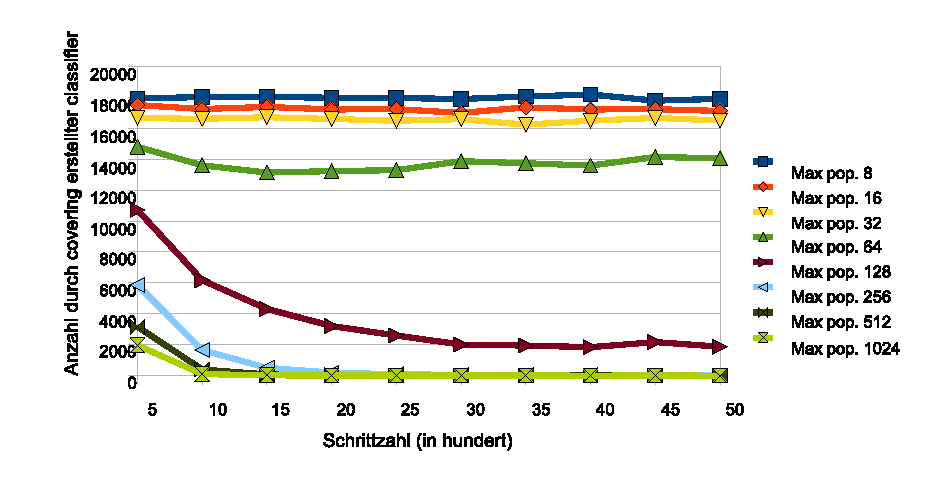
\includegraphics{neuerstellte_classifier_maxpop.eps}
}
\caption[Auswirkung der maximalen Populationsgr��e auf die Anzahl der \emph{classifier} die durch \emph{covering} neuerstellt werden (S�ulenszenario)]{Auswirkung der maximalen Populationsgr��e auf die Anzahl der \emph{classifier} die durch \emph{covering} neuerstellt werden} (S�ulenszenario, Zielobjekt mit einfacher Richtungs�nderung, 8 Agenten mit SXCS)}
\label{neuerstellte_classifier_maxpop:fig}
\end{figure}

Bei der Wahl eines geeigneten Werts spielen au�erdem die Konvergenzgeschwindigkeit und die Laufzeit eine Rolle. Einen allgemein besten Wert f�r \(N\) gibt es nicht, denn er h�ngt insbesondere von der durch das Szenario und der durch die L�nge des \emph{condition} Vektors gegebenen M�glichkeiten ab, also wieviele \emph{classifier} mit verschiedenen \emph{condition} Vektoren und verschiedenem \emph{action} Wert in der \emph{covering} Funktion konstruiert werden k�nnen. W�rde man beispielsweise weitere Zielobjekte auf das Feld setzen, k�nnten eine Reihe weiterer Situationen auftreten, beispielsweise k�nnten Zielobjekte in Sicht in zwei unterschiedlichen Richtungen auftauchen. Selbiges gilt f�r das Szenario ohne Hindernisse, hier f�llt eine ganze Anzahl von M�glichkeiten heraus, was man in Abbildung~\ref{neuerstellte_classifier_maxpop_empty:fig} als Vergleich sehen kann....  Letztlich wei� der Agent nicht, in was f�r einem Szenario er sich befindet, also wie gro� die Menge der \emph{classifier} ist, die das Problem abdecken. Die L�sung w�re eine Populationsgr��e \(N\) die sich flexibel anpasst, dieser Ansatz soll aber hier nicht weiter untersucht werden, stattdessen soll erst ein Blick auf die Laufzeit geworfen werden.\\

\begin{figure}[htbp]
\centerline{	
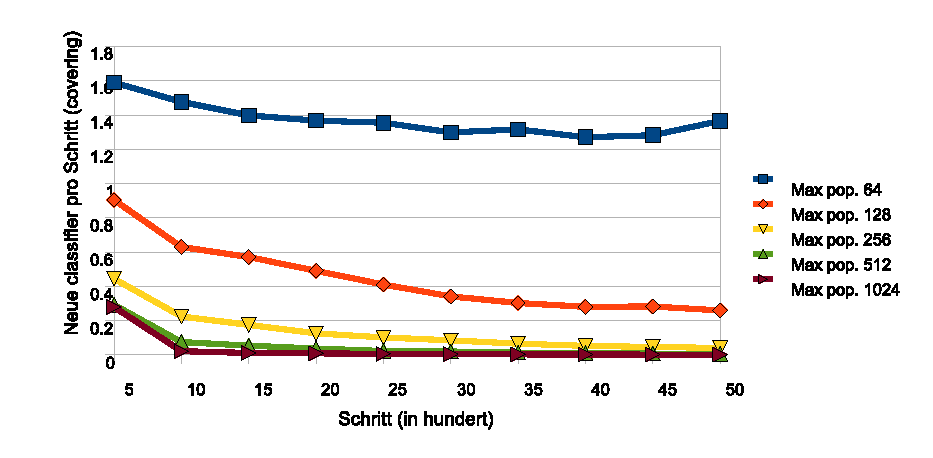
\includegraphics{neuerstellte_classifier_maxpop_empty.eps}
}
\caption[Auswirkung der maximalen Populationsgr��e auf die Anzahl der \emph{classifier} die durch \emph{covering} neuerstellt werden (leeres Szenario)]{Auswirkung der maximalen Populationsgr��e auf die Anzahl der \emph{classifier} die durch \emph{covering} neuerstellt werden} (leeres Szenario ohne Hindernisse, Zielobjekt mit einfacher Richtungs�nderung, 8 Agenten mit SXCS)}
\label{neuerstellte_classifier_maxpop_empty:fig}
\end{figure}

F�r den Overhead (d.h. die Zeit, die 8 Agenten mit zuf�lliger Bewegung ben�tigen) ergab sich eine mittlere Laufzeit von \(1,67\)s pro Experiment bei 500 Schritten (bzw. \(6,50\)s bei 2000 Schritten), was die anf�ngliche Stagnation bis \(N = 32\) erkl�rt. Zieht man diesen von den Messwerten (siehe Abbildung~\ref{empty_grid_time_maxpop:fig}) ab, erh�lt man im betrachteten Wertebereich einen nahezu linearen Verlauf (siehe Abbildung~\ref{linear_pop_time:fig}, ab \(N > 128\)). Der fallende Verlauf bis 128 erkl�rt sich durch den Overhead des XCS Algorithmus selbst.\\

Da also die wichtigsten \emph{classifier} mit Populationsgr��e 256 (bzw. 128 im leeren Szenario) bereits abgedeckt sind, f�hrt eine Erh�hung der Populationsgr��e nur zu einer Erh�hung der Laufzeit. Da den Agenten das Szenario unbekannt ist, soll f�r alle Szenarien der selbe Wert benutzt werden soll. Alles in allem scheint somit \(N = 256\) die schnellste Parametereinstellung zu sein, die gleichzeitig auch ausreichend Platz f�r \emph{classifier} f�r die Abdeckung der M�glichkeiten der betrachteten Szenarien bietet.\\

Die Tests liefen auf einem T7500, 2.2 GHz in einem einzelnen Thread. Als Vergleich hierzu wurde auch der Einfluss der Kartengr��e auf die Laufzeit betrachtet, wie in Abbildung~\ref{time_map_size_correlation:fig} zu sehen, ist der Einfluss auf die Laufzeit im getesteten Bereich (256 - 1024) ohne Bedeutung.\\


\begin{figure}[htbp]
\centerline{	
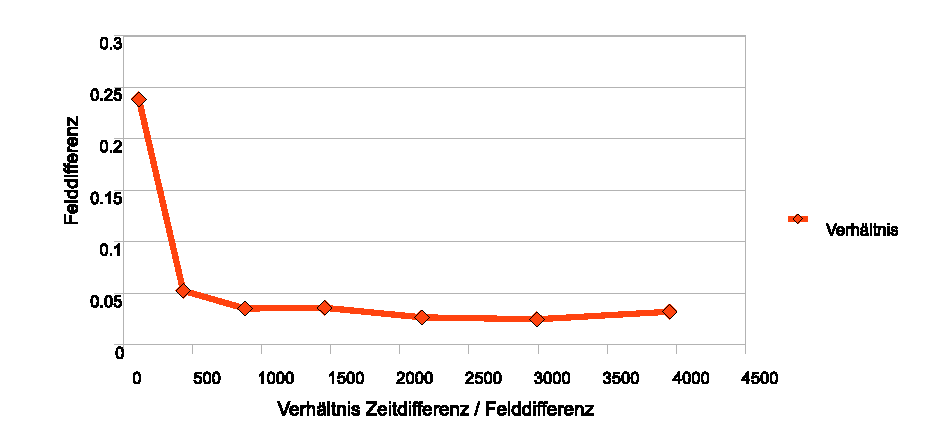
\includegraphics{time_map_size_correlation.eps}
}
\caption[Auswirkung der Torusgr��e auf die Laufzeit (leeres Szenario)] {Darstellung der Auswirkung der Torusgr��e auf die Laufzeit im leeren Szenario, zuf�lliger Bewegung des Zielobjekts, 8 sich zuf�llig bewegenden Agenten}
\label{time_map_size_correlation:fig}
\end{figure}

\begin{figure}[htbp]
\centerline{	
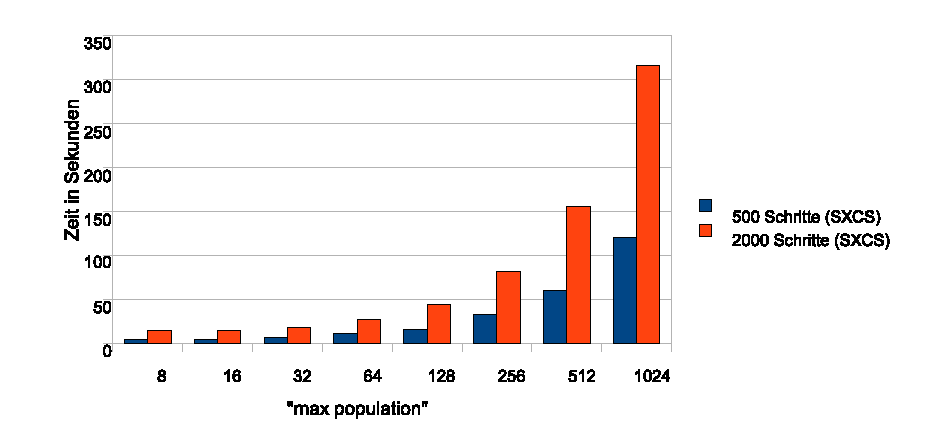
\includegraphics{empty_grid_time_maxpop.eps}
}
\caption[Auswirkung des Parameters \emph{max population N} auf Laufzeit (leeres Szenario)] {Darstellung der Auswirkung des Parameters \emph{max population N} auf die Laufzeit im leeren Szenario, zuf�lliger Bewegung des Zielobjekts, 8 Agenten mit SXCS Algorithmus}
\label{empty_grid_time_maxpop:fig}
\end{figure}

\begin{figure}[htbp]
\centerline{	
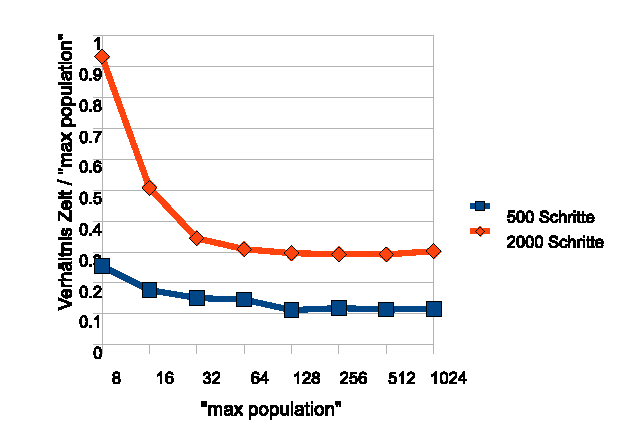
\includegraphics{linear_pop_time.eps}
}
\caption[Verh�ltnis Laufzeit zu \emph{max population N} (leeres Szenario)] {Darstellung der Auswirkung des Parameters \emph{max population N} auf das Verh�ltnis der Laufzeit zu \(N\) im leeren Szenario, zuf�lliger Bewegung des Zielobjekts, 8 Agenten mit SXCS Algorithmus}
\label{linear_pop_time:fig}
\end{figure}


\section{Maximalwert \emph{reward}}\label{sec:maximalwert_rho}

TODO
Der Wert der bei der Bewertung als \emph{reward} vergeben wird hat lediglich �sthetische Auswirkungen und wurde auf \(1.0\) gesetzt. In der Standardimplementation von XCS (siehe Abbildung~\ref{multistep_calc_reward:fig}) ist der maximale \emph{reward} �quivalent mit dem Maximalwert von \(\rho\), da das Problem bei jedem positiven \emph{reward} Wert neugestartet wird, also entweder der \emph{reward} Wert aus dem letzten Schritt also immer \(0\) ist oder \emph{maxPrediction} auf \(0\) gesetzt wurde, und \(\rho = \) \emph{reward} \(+~\gamma \) \emph{maxPrediction} gilt.\\

In den hier vorgestellten XCS Varianten wird dagegen der \emph{reward} Wert absteigend, zusammen mit dem \emph{maxPrediction} Wert, an fr�here \emph{actionSet} Listen verteilt, \(\rho\) kann also gr��er als \(1.0\) werden. In diesem Bereich ist noch Bedarf an theoretischer Forschung, in Tests haben sich Werte bis \(3.0\) ergeben, welche aber vom jeweiligen Szenario abh�ngen. Wird das Zielobjekt (z.B. wegen Hindernissen oder gro�en Torusdimensionen) eher selten gesehen, f�llt der Wert geringer aus.\\


\section{Parameter \emph{accuracy equality} $\epsilon_{0}$}

TODO 
Der Parameter \(\epsilon_{0}\) gibt an, unter welchem Wert zwei \emph{accuracy} Werte als gleich gelten sollen. Dies ist insbesondere bei der \emph{subsummation} Funktion und der Berechnung des \emph{accuracy} Werts von Bedeutung. In der Literatur~\cite{butz01algorithmic} wird als Regel genannt, dass der Wert auf etwa 1\% des Maximalwerts von \(\rho\) gesetzt werden soll, den der erwartete \emph{reward} annehmen kann. Aufgrund der �berlegungen in~\ref{sec:maximalwert_rho} wird \(\epsilon_{0}\) f�r die neuen XCS Varianten auf \(0.02\) gesetzt, w�hrend es f�r die Standardimplementation von XCS auf \(0.01\) gesetzt wird. Ein Testdurchlauf auf dem S�ulenszenario (siehe Abbildung~\ref{pillar_epsilon0:fig}) ergibt aber, dass der Parameter keine besondere Auswirkung hat, weshalb der Wert auf \(0.01\) belassen wird.

\begin{figure}[htbp]
\centerline{	
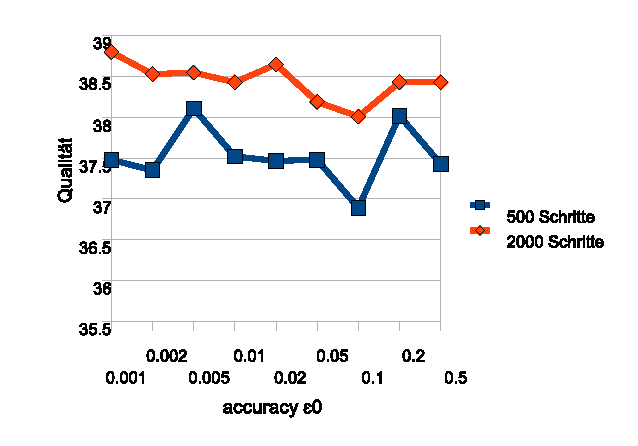
\includegraphics{pillar_epsilon0.eps}
}
\caption[Auswirkung des Parameters \emph{accuracy equality} $\epsilon_{0}$ auf die Qualit�t (S�ulenszenario)] {Auswirkung des Parameters  \emph{accuracy equality} $\epsilon_{0}$ auf die Qualit�t im S�ulenszenario, zuf�lliger Bewegung des Zielobjekts, 8 Agenten mit SXCS Algorithmus}
\label{pillar_epsilon0:fig}
\end{figure}


\section{Parameter \emph{reward prediction discount} $\gamma$}


%%sxcs gut: 0.4 p#, kein random start, kein GA
dsxcs gut: alles an TODO maxpred �berpr�fen...


Der Einfluss von \(\gamma\) ist zwar vorhanden, aber sehr gering. 
TODO

TODO Reward prediction unn�tig bei speed 2, pillar, random

TODO Abschnitt entfernen
Auch f�r den Wert \emph{reward prediction discount} \(\gamma\) hat sich ein etwas h�herer Wert als sinnvoll erwiesen, als standardm��ig benutzt wird. Laut~\cite{butz01algorithmic} h�ngt der Wert auch vom verwendeten Szenario ab. Ein h�herer Wert f�r \(\gamma\) bedeutet, dass die H�he des Werts, der �ber \emph{maxPrediction} weitergegeben wird, mit zeitlichem Abstand zur urspr�nglichen Bewertung mit einem \emph{reward}, weniger schnell abf�llt, wodurch eine l�ngere Verkettung von \emph{reward} Werten m�glich ist. Umgekehrt f�hren zu hohe Werte f�r \(\gamma\) zu der positiven Bewertung von \emph{classifiers} die am Erfolg gar nicht beteiligt waren, was sich negativ auf die Qualit�t auswirken kann.

Tabelle~\ref{table:prediction_discount} zeigt einen Vergleich der Qualit�t mit dem Standardwert \(\gamma = 0.71\) und dem f�r die in dieser Arbeit verwendeten Testszenarien gew�hlten Wert \(\gamma = 0.95\).\\

TODO 0.71 lassen

auch mit Geschwindigkeit 0.1 oder so testen

TODOTabelle prediction discount


\section{Parameter Lernrate $\beta$}\label{sec:learnrate_parameter}

F�r die Lernrate \(\beta\) hat sich ein etwas niedrigerer als in der Literatur angegebener Wert (\(0.01\)) als erfolgreich erwiesen. Die Lernrate bestimmt, wie stark ein ermittelter \emph{reward} Wert den \emph{reward prediction}, \emph{reward prediction error}, \emph{fitness} und \emph{action set size} Wert pro Aktualisierung beeinflusst.TODO
Auch dieser Parameter ist szenariospezifisch, �ber die konkrete Begr�ndung kann nur spekuliert werden, die Schwierigkeit des Szenarios 
TODO

Vergleichende Tests (siehe Abbildung~\ref{pillar_learning_rate_quality:fig} mit niedrigerem bzw. h�herem Wert haben zu einer etwas schlechteren Qualit�t gef�hrt. TODO

\begin{figure}[htbp]
\centerline{	
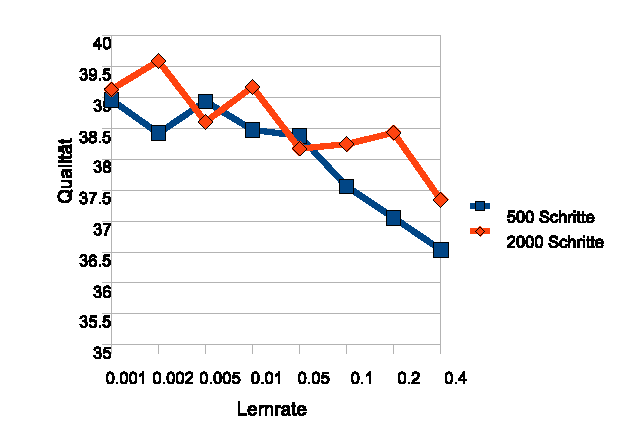
\includegraphics{pillar_learning_rate_quality.eps}
}
\caption[Auswirkung des Parameters \emph{learning rate} $\beta$ auf Qualit�t (S�ulenszenario)] {Auswirkung des Parameters \emph{learning rate} $\beta$ auf die Qualit�t im S�ulenszenario, zuf�lliger Bewegung des Zielobjekts, 8 Agenten mit SXCS Algorithmus}
\label{pillar_learning_rate_quality:fig}
\end{figure}



\section{Parameter \emph{reward prediction init} $p_{i}$}\label{prediction_init:sec}

In der Literatur werden Werte nahe Null bzw. 1\% von \(\rho\) als Initialisierung f�r den \emph{reward prediction} Wert eines \emph{classifiers} angegeben. Im in dieser Arbeit untersuchten Fall, bei dem die Agenten nur begrenzte Sensorf�higkeiten besitzen, sich auf einem Torus frei bewegen k�nnen und keine festen Pfade suchen m�ssen, ist zu erwarten, dass sich die \emph{reward prediction} Werte der einzelnen \emph{classifier} untereinander wenig unterscheiden, w�hrend sie beispielsweise bei statischen Szenarien gegen feste, stark unterschiedliche Werte konvergieren. Beispielsweise im Einf�hrungsbeispiel in Abbildung~\ref{simple_scenario_multistep:fig} w�rden die \emph{reward prediction} Werte der \emph{classifier} b), c), e) und g) eher gegen 1 und die der restlichen \emph{classifier} gegen 0 streben.\\
Welchen Wert man f�r \(p_{i}\) nun als Durchschnittswert w�hlt, h�ngt vom jeweiligen Szenario ab. Beispielsweise w�rde ein �berwachungsszenario auf einem sehr gr��eren Torus mit relativ wenigen Agenten w�rde zu einem niedrigeren Durchschnittswert f�r die \emph{reward prediction} Variable f�hren und umgekehrt.\\
Einfache Idee ist deshalb, auszunutzen, dass im jeweiligen \emph{classifier set} bereits die Information enthalten ist, was der Durchschnittswert f�r das aktuelle Szenario ist, n�mlich der Durchschnittswert aller \emph{reward prediction} Werte. Dies kann man noch dadurch erweitern, dass man bei der Durchschnittsbildung nur solche \emph{classifier} miteinbezieht, welche einen ausreichend gro�en \emph{experience} Wert besitzen.\\

Tests haben gezeigt, dass dadurch ein deutlich schnelleres Konvergenzverhalten erreicht werden konnte

TODO Test

TODO raus unten
W�hlt man einen Wert, der n�her am Durchschnitt der \emph{reward prediction} Werte der \emph{classifier} liegt, die sich in den besten L�sungen am Ende eines Testdurchlaufs befinden, so ist zu erwarten, dass die Anzahl der ben�tigten Aktualisierungen des \emph{reward prediction} Werts geringer ausf�llt, das System also schneller konvergiert. Diese �berlegung wird best�tigt durch entsprechende Tests (siehe~\ref{pillar_lcs_prediction_init_quality:fig}).\\
Wir setzen somit f�r SXCS den Parameter auf \(p_{i} = 1.0\).\\
Zu beachten ist, dass diese �berlegung prim�r deswegen gilt, weil die 


TODO Standardverfahren?

\begin{figure}[htbp]
\centerline{	
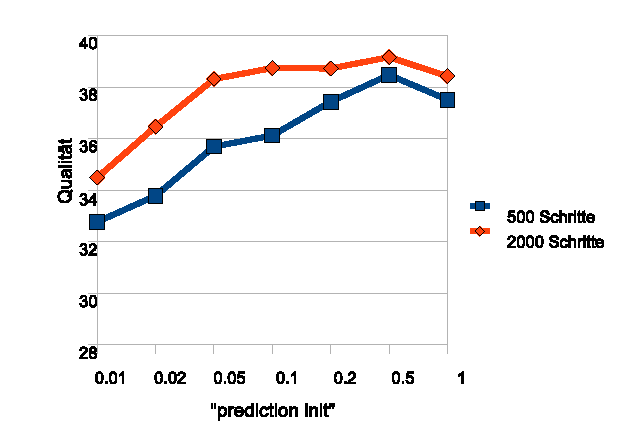
\includegraphics{pillar_lcs_prediction_init_quality.eps}
}
\caption[Auswirkung des Parameters \emph{reward prediction init} $p_{i}$ auf Qualit�t (S�ulenszenario)] {Darstellung Auswirkung des Parameters \emph{reward prediction init} $p_{i}$ auf die Qualit�t im S�ulenszenario, zuf�lliger Bewegung des Zielobjekts, 8 Agenten mit SXCS Algorithmus}
\label{pillar_lcs_prediction_init_quality:fig}
\end{figure}


\section{Zuf�llige Initialisierung der \emph{classifier set} Liste}\label{sec:random_init}

Normalerweise werden XCS Systeme mit leeren \emph{classifier set} Listen initialisiert, als Option wird jedoch auch eine zuf�llige Initialisierung erw�hnt~(\cite{Butz2006}), bei der zu Beginn die \emph{classifier set} Liste mit mehreren \emph{classifiers} mit zuf�lligen \emph{action} Werten und \emph{condition} Vektoren gef�llt wird. Dort wird aber auch angemerkt, dass beide Varianten in ihrer Qualit�t sich nur minimal unterscheiden.\\

Tests f�r das �berwachungsszenario haben gezeigt (siehe Tabelle~\ref{table:lcs_initialization}), dass dadurch minimal bessere Ergebnisse erzielt werden, allerdings nur in Szenarien mit ausreichender Schrittzahl (\(>100\)). Dies l�sst sich darauf zur�ckf�hren, dass  anf�nglich gef�llte \emph{classifier set} Listen die \emph{matchSet} Listen relativ gro� lassen werden, somit die Auswirkungen anf�nglichen Lernens geringer ausfallen und sich die Agenten eher wie sich zuf�llig bewegende Agenten verhalten. Da hier durchgef�hrten Tests �ber 500 bzw. 2000 Schritte laufen, sollen somit die \emph{classifier set} Listen mit zuf�llig generierten \emph{classifiers} gef�llt werden.\\

Au�erdem hat eine Analyse der sich am Schluss ergebenen \emph{classifier set} Listen ergeben, dass sich dort in bestimmten Szenarien eine ganze Reihe von \emph{classifier} mit einem \emph{experience} Wert von 0 befinden. Eine genauere Betrachtung des \emph{condition} Vektors zeigte den Grund daf�r, die dort beschriebene Situation konnte in dem Szenario nicht auftreten (z.B. im schwierigen Szenario eine Situation ohne Hindernisse in Sicht). Tritt die Situation nie auf, kann der \emph{classifier} auch keine Erfahrung gewinnen und wird mangels ausreichend hohem \emph{experience} Wert auch nicht bei der L�schung ber�cksichtigt, der \emph{classifier} bleibt also f�r immer im \emph{classifier set}. Um dieses Problem in Verbindung mit der zuf�lligen Initialisierung zu umgehen, sollen alle
TODO nein

\begin{table}[ht]
\caption{Vergleichende Tests f�r den den Start mit und ohne zuf�llig gef�llten \emph{classifier set} Listen}
\centering
\begin{tabular}{c c c c c}
\hline
Algorithmus & Agentenzahl & Schrittzahl & Abdeckung & Qualit�t \\ [0.5ex]
\hline
Zuf�lliger Agent & 8 & 500 & 60.64\% & 61.54\% \\
Multistep & 8 & 500 & 60.64\% & 61.54\% \\
LCS & 8 & 500 & 60.64\% & 61.54\% \\
NewLCS & 8 & 500 & 60.64\% & 61.54\% \\
Zuf�lliges Szenario  & 8 & 500 & 60.64\% & 61.54\% \\
S�ulenszenario & 8 & 100 & 1.0\% & 1.0\% \\
LCS Ohne Drehung & 8 & 2000 & 1.0\% & 1.0\% \\ [0.5ex]

LCS Mit Drehung & 8 & 100 & 1.0\% & 1.0\% \\
LCS Mit Drehung & 8 & 500 & 1.0\% & 1.0\% \\
LCS Mit Drehung & 8 & 2000 & 1.0\% & 1.0\% \\ [0.5ex]

Zuf�lliger Agent & 12 & 500 & 76.03\% & 76.59\% \\
Einfacher Agent & 12 & 500 & 67.30\% & 96.86\% \\
Intelligenter Agent & 12 & 500 & 86.85\% & 95.08\% \\ [0.5ex]

LCS Ohne Drehung & 12 & 100 & 1.0\% & 1.0\% \\
LCS Ohne Drehung & 12 & 500 & 1.0\% & 1.0\% \\
LCS Ohne Drehung & 12 & 2000 & 1.0\% & 1.0\% \\ [0.5ex]

LCS Mit Drehung & 12 & 100 & 1.0\% & 1.0\% \\
LCS Mit Drehung & 12 & 500 & 1.0\% & 1.0\% \\
LCS Mit Drehung & 12 & 2000 & 1.0\% & 1.0\% \\ [0.5ex]

\hline
\end{tabular}
\label{table:lcs_initialization}
\end{table}


\section{�bersicht �ber alle Parameterwerte}
\begin{table}[ht]
\caption{Verwendete Parameter (soweit nicht anders angegeben) und Standardparameter, TODO englisch/deutsch}
\centering
\begin{tabular}{c c c}
\hline\hline
Parameter & Wert & Standardwert (siehe~\cite{butz01algorithmic})\\ [0.5ex]
\hline
Max population \(N\) & \textbf{128} (siehe Kapitel~\ref{sec:max_population_parameter})\\
Max value \(\rho\) & \textbf{1.0} (siehe Kapitel~\ref{sec:maximalwert_rho}) & [10000]\\
Fraction mean fitness \(\delta\) & 0.1 & [0.1]\\
Deletion threshold \(\theta_{\mathrm{del}}\) & 20.0 & [\(\sim\) 20.0]\\
Subsumption threshold \(\theta_{\mathrm{sub}}\) & 20.0 & [20.0+]\\
Covering \(\#\) probability \(P_{\#}\) & 0.5 & [\(\sim\) 0.33]\\
GAthreshold \(\theta_{\mathrm{GA}}\) & 25.0 & [25-50]\\
Mutation probability \(\mu\) & \(0.05\) & [0.01-0.05]\\
Prediction error reduction & 0.25 & [0.25]\\
Fitness reduction & \(0.1\) & [0.1]\\

Reward prediction init \(p_{i}\) & \textbf{0.5, 1.0} (siehe~\ref{prediction_init:sec}) & [\(\sim\) 0]\\
Prediction error init \(\epsilon_{i}\) & 0.0 & [0.0]\\
Fitness init \(F_{i}\) & \(0.01\) &  [0.01]\\
Condition vector & \textbf{zuf�llig} (siehe Kapitel~\ref{sec:random_init}) &  [zuf�llig oder leer]\\
Numerosity & 1 & [1]\\
Experience & 0 & [0]\\

Accuracy equality \(\epsilon_{0}\) & \textbf{0.05} & [\emph{1\% des gr��ten Werts}]\\
Accuracy calculation \(\alpha\) & 0.1 & [0.1]\\
Accuracy power \(\nu\) & 5.0 & [5.0]\\
Reward prediction discount \(\gamma\) & 0.71 & [0.71]\\

Learning rate \(\beta\) & \textbf{0.01} (siehe~\ref{sec:learnrate_parameter}) & [0.1-0.2]\\

exploration probability & 0.5 (siehe~\ref{subsummation:sec}) & [\(\sim\) 0.5]\\ [0.5ex]

\hline
\end{tabular}
\label{table:lcs_parameter}
\end{table}





\chapter{XCS}\label{lcs:cha}

\section{Einf�hrung}

Jeder Agent besitzt ein sogennantes \emph{XCS Classifier System} welches einem speziellen \emph{learning classifier system} (LCS) entspricht. Ein LCS ist ein evolution�res Lernsystem, das aus einer Reihe von \emph{classifier} Regeln besteht (siehe Kapitel~\ref{uebersicht_classifier:sec}). Eine allgemeine Einf�hrung in LCS findet sich z.B. in~\cite{Butz2006a}.\\

Eine wesentliche Erweiterung des LCS ist das sogenannte ``accuracy-based classifier system XCS'', zuerst beschrieben in \cite{Wilson1995}. Neben neuer  Mechanismen zur Generierung neuer \emph{classifier} (insbesondere im Bereich bei der Anwendung des genetischen Operators) ist im Vergleich zum einfachen LCS der wesentliche Unterschied, auf welche Weise der \emph{fitness} Wert berechnet wird. W�hrend der \emph{fitness} Wert beim einfachen LCS lediglich auf dem \emph{reward prediction error} Wert basierte, basiert bei XCS der \emph{fitness} Wert auf der Genauigkeit der jeweiligen Regel. Eine genaue Beschreibung findet sich in~\cite{Butz2006}.\\

Im einfachsten Fall, im sogenannten ``Single-Step''-Verfahren erfolgt die Bewertung einzelner \emph{classifier}, also der Bestimmung eines jeweils neuen \emph{fitness} Werts, sofort nach Aufruf jeder einzelnen Regel, w�hrend im sogenannten ``Multi-Step''-Verfahren mehrere aufeinanderfolgende Regeln erst dann bewertet werden, sobald ein Ziel erreicht wurde. Ein klassisches Beispiel f�r den Test ``Single-Step''-Verfahren ist das 6-Multiplexer Problem (z.B. in ~\cite{Butz2006}), bei dem mit 2 Adressbits und 4 Datenbits das den Adressbits entsprechende ausgegeben werden soll. Hier ist offensichtlich, dass nach der Klassifizierung sofort bestimmbar ist, ob sie ein korrektes Ergebnis geliefert hat.\\
Ein klassisches Beispiel f�r ``Multi-Step''-Verfahren ist das ``Maze~\(N\)'' Problem, bei dem durch ein Labyrinth mit dem k�rzesten Weg von \(N\) Schritten gegangen werden muss. Am Ziel angekommen wird der zuletzt aktivierte \emph{classifier} positiv bewertet und das Problem wiederholt. Bei den Wiederholungen erh�lt jede Regel einen Teil der Bewertung des folgenden \emph{classifiers}. Somit wird eine ganze Kette von \emph{classifier} bewertet und sich der optimalen Wahrscheinlichkeitsverteilung angen�hert, welche repr�sentiert, welche der Regeln in welchem Ma� am L�sungsweg beteiligt sind.\\

Die in dieser Arbeit verwendete Implementierung entspricht im Wesentlichen der Standardimplementation des Multistep-Verfahrens von~\cite{Butz2000} (mit der algorithmischen Beschreibung des Algorithmus in ~\cite{Butz}), eine Besonderheit stellt allerdings die Problemdefinition dar, da es kein festes Ziel gibt und somit auch keinen Neustart des Problems.\\

Die meisten Implementationen und Varianten von XCS besch�ftigen sich mit Szenarios, bei denen das Ziel in einer statischen Umgebung gefunden werden muss. H�ufiger Gegenstand der Untersuchung in der Literatur sind insbesondere relativ einfache Probleme 6-Multiplexer Problem und Maze1 (z.B. in ~\cite{Butz2006} \cite{xcs1} \cite{xcs2}), w�hrend XCS mit Problemen gr��erer Schrittzahl zwischen Start und Ziel Probleme hat \cite{Barry} \cite{Banzhaf}. Zwar gibt es Ans�tze um auch schwierigere Probleme besser in den Griff zu bekommen (z.B. Maze5, Maze6, Woods14 in~\cite{Butz2005}), indem ein Gradientenabstieg in XCS implementiert wurde. Ein konkreter Bezug zu einem dynamischen �berwachungsszenario konnte jedoch in keiner dieser Arbeiten gefunden werden.\\

Bez�glich Multiagentensystemen und XCS gibt es haupts�chlich Arbeiten, die auf  auf zentraler Steuerung bzw. \emph{OCS} \cite{Takadama} basieren, also im Gegensatz zum Gegenstand dieser Arbeit auf eine �bergeordnete Organisationseinheit bzw. auf globale Regeln oder globalem Regeltausch zwischen den Agenten zur�ckgreifen.\\
Arbeiten bez�glich Multiagentensysteme in Verbindung mit LCS im Allgemeinen finden sich z.B. in \cite{Benouhiba}, wobei es auch dort zentrale Agenten gibt, mit deren Hilfe die Zusammenarbeit koordiniert werden soll, w�hrend in dieser Arbeit alle Agenten die selbe Rolle spielen sollen.\\

Vielversprechend war der Titel der Arbeit~\cite{Lujan}, ``Generation of Rule-based Adaptive Strategies for a Collaborative Virtual Simulation Environment''. Leider wird in der Arbeit nicht diskutiert, auf was sich der kollaborative Anteil bezog, da nicht mehrere Agenten benutzt worden sind. Auch konnte dort jeder einzelne Schritt mittels einer \emph{reward} Funktion bewertet werden, da es globale Information gab. Dies vereinfacht ein solches Problem deutlich und macht einen Vergleich schwierig.\\

Eine weitere Arbeit in dieser Richtung (\cite{elfarol}) beschreibt das ``El Farol'' Bar Problem, welches dort mit Hilfe eines Multiagenten XCS System erfolgreich gel�st wurde. Die Vergleichbarkeit ist hier auch eingeschr�nkt, da es sich bei dem EFBP um ein ``Single-Step'' Problem handelt.\\

Eine der dieser Arbeit (bez�glich Multiagentensysteme) am n�chsten kommende Problemstellung wurde in \cite{Hiroyashu} vorgestellt. Dort wurde der \emph{base reward} unter den (zwei) Agenten aufgeteilt, es fand also eine Kommunikation des \emph{reward} Werts statt. Wie das Ergebnis in Verbindung mit den Ergebnissen dieser Arbeit interpretiert werden kann, wird in~\ref{communication:cha} diskutiert.\\

In \cite{Miyazaki} wurde gezeigt, dass bei der Weitergabe des \emph{base reward} Gruppenbildung von entscheidender Wichtigkeit ist. Nach bestimmten Kriterien werden Agenten in Gruppen zusammengefasst und der \emph{base reward} anstatt an alle, jeweils nur an die jeweiligen Gruppenmitgliedern weitergegeben.
Dies best�tigen auch Tests in Kapitel~\ref{communication:cha} bei der sich Agenten mit �hnelnden (was das Verhalten gegen�ber anderen Agenten betrifft) \emph{classifier sets} in Gruppen zusammengefasst wurden und zum Teil bessere Ergebnisse erzielt werden konnten als ohne Kommunikation.

\section{�bersicht}\label{uebersicht_classifier:sec}

TODO base reward und reward unterscheiden

Ein XCS ist ein regelbasiertes evolution�res Lernsystem, das im Wesentlichen aus folgenden Elementen besteht:

\begin{enumerate}
\item Einer Menge an Regeln, sogenannte \emph{classifier} (siehe~\ref{classifier:sec})
\item Ein Mechanismus zur Auswahl der \emph{classifier} (siehe~\ref{auswahlart:sec})
\item Einem Mechanismus zur Evolution der \emph{classifier} (mittels genetischer Operatoren, siehe~\ref{genetische_operatoren:sec})
\item Eine Mechanismus zur Bewertung der \emph{classifier} (mittels \emph{reinforcement learning}, siehe~\ref{bewertung:sec})
\end{enumerate}

W�hrend die ersten drei Punkten bei allen hier vorgestellten XCS Varianten identisch sind, gibt es wesentliche Unterschiede bei der Bewertung der \emph{classifier}. Diese werden gesondert in Kapitel~\ref{lcs_variants:cha} im Einzelnen besprochen. Im Folgenden sollen nun die ersten drei Punkte n�her betrachtet werden.

\section{Classifier}\label{classifier:sec}

Ein \emph{classifier} besteht aus einem \emph{condition} Vektor, einem \emph{action}, einem \emph{fitness}, einem \emph{reward prediction}, einem \emph{reward prediction error}, einem \emph{experience} und einem \emph{actionSetSize} Wert. Initialisiert werden diese Teile wie in~\ref{cha:parameter} aufgelistet.

\subsection{Der \emph{action} Wert}
Wird ein \emph{classifier} ausgew�hlt, wird eine bestimmte Aktion ausgef�hrt die durch den \emph{action} Wert determiniert ist. Im Rahmen dieser Arbeit entsprechen diese Aktionsm�glichkeiten den 4 Bewegungsrichtungen, die in Kapitel~\ref{agent_abilities:sec} besprochen wurden.

\subsection{Der \emph{fitness} Wert}
Der \emph{fitness} Wert soll die allgemeine Genauigkeit des \emph{classifier}
repr�sentieren und wird �ber die Zeit hinweg sukzessive an die beobachteten \emph{reward} Werte angepasst. Der Wertebereich verl�uft zwischen \(0.0\) und \(1.0\) (maximale Genauigkeit). Insbesondere eines der fr�hesten Werke zu XCS \cite{Wilson} besch�ftigte sich mit diesem Aspekt der Genauigkeit.

\subsection{Der \emph{reward prediction} Wert}
Der \emph{reward prediction} Wert des \emph{classifier} stellt die H�he des \emph{reward} Werts dar, von dem der \emph{classifier} erwartet, dass er ihn bei der n�chsten Bewertung erhalten wird.

\subsection{Der \emph{reward prediction error} Wert}
Der \emph{reward prediction error} Wert soll die Genauigkeit des \emph{classifier} bzgl. des \emph{reward prediction} Werts (durchschnittliche Differenz zwischen \emph{reward prediction} und tats�chlichem \emph{reward}) repr�sentieren. U.a. auf Basis dieses Werts wird der \emph{fitness} Wert des \emph{classifier} angepasst.

\subsection{Der \emph{condition} Vektor}\label{condition_vector:sec}
Der \emph{condition} Vektor gibt die Kondition an, in welcher Situation der zugeh�rige \emph{classifier} ausgew�hlt werden kann, d.h. welche Sensordaten von dem jeweiligen \emph{classifier} erkannt werden. Alle \emph{classifier} die einen Sensordatensatz erkennen bilden das sogenannte \emph{matchSet}. Der Aufbau des Vektors entspricht dem Vektor der �ber die Sensoren erstellt wird (siehe~\ref{sensoren:sec}).

\[
\underbrace{z_{s_{N}} z_{r_{N}} z_{s_{O}} z_{r_{O}} z_{s_{S}} z_{r_{S}} z_{s_{W}} z_{r_{W}}}_{Erste~Gruppe~(Zielobjekt)}
\underbrace{a_{s_{N}} a_{r_{N}} a_{s_{O}} a_{r_{O}} a_{s_{S}} a_{r_{S}} a_{s_{W}} a_{r_{W}}}_{Zweite~Gruppe~(Agenten)}
\underbrace{h_{s_{N}} h_{r_{N}} h_{s_{O}} h_{r_{O}} h_{s_{S}} h_{r_{S}} h_{s_{W}} h_{r_{W}}}_{Dritte~Gruppe~(Hindernisse)}
\]


\section{Platzhalter im \emph{condition} Vektor}\label{platzhalter:sec}

Neben den zu den Sensordaten korrespondierenden Werten 0 und 1 soll es noch einen dritten Zustand, den Platzhalter ``\#'', geben, der anzeigen soll, dass beim Vergleich zwischen Kondition und Sensordaten diese Stelle ignoriert werden soll. Eine Stelle im \emph{condition} Vektor mit Platzhalter gilt also als �quivalent zur korrespondierenden Stelle in den Sensordaten, egal ob sie mit 0 oder 1 belegt ist. Ein Vektor, der ausschlie�lich aus Platzhaltern besteht, w�rde somit bei der Auswahl immer in Betracht gezogen werden, da er auf alle m�glichen Kombinationen der Sensordaten passt.\\
Beim Vergleich der Sensordaten und Daten aus dem \emph{condition} Vektor werden immer jeweils zwei Paare verglichen. In~\ref{sensoren:sec} wurde erw�hnt, dass der Fall \((0/1\)) in den Sensordaten nicht auftreten kann, weswegen (um die Aufgabe nicht unn�tig zu erschweren) ein Datenpaar \((0/1\)) im \emph{condition} Vektor �quivalent zum Datenpaar \((1/1\)) sein soll, es damit also eine gewisse Redundanz gibt.

\begin{enumerate}
\item Sensorenpaar \((0/0)\) wird erkannt von \((0/0)\), \((\#, 0)\), \((0, \#)\), \((\#, \#)\)
\item Sensorenpaar \((1/0)\) wird erkannt von \((1/0)\), \((\#, 0)\), \((1, \#)\), \((\#, \#)\)
\item Sensorenpaar \((1/1)\) wird erkannt von \((1/1)\), \((\#, 1)\), \((1, \#)\), \((\#, \#)\), \((0/1)\)
\end{enumerate}

Beispielsweise w�rden folgende Sensordaten von den folgenden \emph{condition} Vektoren erkannt:
\begin{verbatim}
Sensordaten:
(Zielobjekt in Sicht im Norden, Agent im Sicht im S�den, 
Hindernisse im Westen und Osten)
10 00 00 00 . 00 00 11 00 . 00 11 00 11

Beispiele f�r erkennende condition Vektoren:
10 00 00 00 . ## ## ## ## . 00 ## ## ##
## ## ## ## . ## ## #1 00 . 00 11 ## ##
#0 ## ## ## . ## ## 01 ## . ## 11 ## 11
\end{verbatim}

\section{Subsummation}\label{subsummation:sec}

Die Benutzung von Platzhaltern erlaubt es dem LCS mehrere \emph{classifiers} zu subsummieren, wodurch die Gesamtzahl der \emph{classifier} sinkt und somit Erfahrungen, die ein LCS Agent sammelt, nicht unbedingt mehrfach gemacht werden m�ssen. Die dahinter stehende Annahme ist, dass es Situationen gibt, in denen der Gewinn der durch Unterscheidung zwischen zwei verschiedenen Sensordatens�tzen geringer ist als die Ersparnis durch das Zusammenlegen beider \emph{classifiers}, d.h. dem Ignorieren der Unterschiede.\\

Besitzt ein \emph{classifier} zum einen einen gen�gend gro�en \emph{experience} Wert und ausreichend kleinen \emph{reward prediction error} Wert, so kann er als sogenannter \emph{subsumer} auftreten. Andere \emph{classifiers} mit gleichem \emph{action} Wert werden durch den \emph{subsumer} ersetzt, sofern der von ihnen abgedeckte Sensordatenbereich eine Teilmenge des von dem \emph{subsumer} abgedeckten Bereichs ist, der \emph{subsumer} also an allen Stellen des \emph{condition} Vektors entweder den selben Wert wie der zu subsummierende \emph{classifier} oder einen Platzhalter besitzt.\\

\section{Genetische Operatoren}\label{genetische_operatoren:sec}

Es werden aus den jeweiligen \emph{actionSets} zwei \emph{classifier} (die Eltern) zuf�llig ausgew�hlt und zwei neue \emph{classifier} (die Kinder) aus ihnen gebildet und in die Population eingef�gt. Dabei wird mittels \emph{two-point crossover} ein neuer \emph{condition} Vektor generiert und der \emph{action} Wert auf den der Eltern gesetzt (da sie aus dem selben \emph{actionSet} stammen, ist der Wert beider Eltern identisch). Die restlichen Werte werden standardm��ig wie in Kapitel~\ref{cha:parameter} aufgelistet initialisiert. Werden Kinder in die Population eingef�gt, deren \emph{action} Wert und \emph{condition} Vektor identisch mit existierenden \emph{classifiers} ist, werden sie stattdessen subsummiert.\\
Da die Sensoren und somit auch der \emph{condition} Vektor aus drei in sich geschlossenen Gruppen bestehen, werden im Unterschied zur Standardimplementation beim \emph{crossing over} zwei feste Stellen benutzt, die die Gruppe f�r das Zielobjekt, die Gruppe f�r Agenten und die Gruppe f�r feste Hindernisse voneinander trennen.\\
Bezeichne \((z_1, a_1, h_1)\) bzw. \((z_2, a_2, h_2)\) jeweils die drei Gruppen (siehe~\ref{condition_vector:sec}) des \emph{condition} Vektors des ersten bzw. zweiten ausgew�hlten Elternteils, dann k�nnen f�r die drei Gruppen der \emph{condition} Vektoren \((z_{1k}, a_{1k}, h_{1k})\) und \((z_{2k}, a_{2k}, h_{2k})\) der beiden Kinder folgende Kombinationen auftreten:

\[[(z_{1k}, a_{1k}, h_{1k}), (z_{2k}, a_{2k}, h_{2k})] = [(z_1, a_1, h_1) , (z_2, a_2, h_2)]\]
\[[(z_{1k}, a_{1k}, h_{1k}), (z_{2k}, a_{2k}, h_{2k})] = [(z_2, a_1, h_1) , (z_1, a_2, h_2)]\]
\[[(z_{1k}, a_{1k}, h_{1k}), (z_{2k}, a_{2k}, h_{2k})] = [(z_1, a_2, h_1) , (z_2, a_1, h_2)]\]
\[[(z_{1k}, a_{1k}, h_{1k}), (z_{2k}, a_{2k}, h_{2k})] = [(z_2, a_2, h_1) , (z_1, a_1, h_2)]\]

\section{Der \emph{numerosity} Wert}

Durch Subsummation (siehe~\ref{subsummation:sec} und \ref{genetische_operatoren:sec}) k�nnen \emph{classifier} eine Rolle als \emph{macro classifier} spielen, d.h. \emph{classifier} die andere \emph{classifier} in sich beinhalten. Der \emph{numerosity} Wert gibt an, wieviele andere, sogenannte \emph{micro classifier} sich in dem jeweiligen \emph{classifier} befinden.\\
Durch die Benutzung von \emph{macro classifiers} ergibt sich allerdings das programmiertechnische Problem, dass man nicht mehr direkt wei�, wieviele \emph{micro classifiers} sich in einer Population befinden, bei jeder Benutzung des Werts der Populationsgr��e m�ssten die \emph{numerosity} Werte aller \emph{classifiers} jedes Mal addiert werden. In der Standardimplementierung \cite{Butz2000} ist die Behandlung des \emph{numerosity} Werts deswegen stark optimiert, jedes \emph{classifier set} tr�gt eine tempor�re Variable \emph{numerositySum} mit sich, in der die aktuelle Summe gespeichert ist. Die Aktualisierung ist jedoch zum einen mangelhaft umgesetzt, zum anderen auf die Verwendung von einem einzelnen \emph{actionSet} optimiert, w�hrend die hier verwendete Implementierung jeweils mit bis �ber 100 \emph{actionSets} programmiert wurde, denen ein \emph{classifier} Mitglied sein kann. Deswegen wurde die Optimierung entfernt und durch eine dezentrale Verwaltung mit einem \emph{Observer} ersetzt, jede �nderung des \emph{numerosity} Wertes hat also die �nderung aller \emph{actionSets} zur Folge, in der der \emph{classifier} Mitglied ist.\\
Wird also z.B. ein \emph{micro classifier} entfernt, dann wird lediglich die �nderungsfunktion des \emph{classifiers} aufgerufen, der dann wiederum den \emph{numerositySum} Wert der jeweiligen Eltern anpasst. Dies macht einige Optimierungen r�ckg�ngig, erspart aber sehr viel Umst�nde, den \emph{numerositySum} der Eltern immer auf den aktuellen Stand zu halten und einzelne \emph{classifiers} zu l�schen.\\
Positiver Nebeneffekt durch die verbesserte Struktur, dass man dadurch leicht auf die Menge der \emph{actionSets} zugreifen kann, denen ein \emph{classifier} angeh�rt, hierf�r wurde aber keine Verwendung gefunden.\\

Ein weiteres Problem der Standardimplementierung ist, dass der \emph{fitness} Wert eines \emph{classifiers} als Optimierung bereits den \emph{numerosity} Wert als Faktor enth�lt, w�hrend bei der Aktualisierung des \emph{numerosity} Werts der \emph{fitness} Wert nicht aktualisiert wurde. Das hat zur Folge, dass theoretisch \emph{fitness} Werte von \emph{classifiers} fast den \emph{max population} Wert annehmen kann, wenn ein \emph{classifier} mit \emph{numerosity} und \emph{fitness} Wert in der H�he von \emph{max population} auf einen \emph{numerosity} Wert von 1 reduziert wird.\\
Dies betrifft die Funktion \emph{public void addNumerosity(int num)} der Klasse \emph{XClassifier} in der Datei \emph{XClassifier.java}. Die korrigierte Fassung ist in~\ref{corrected_numerosity_function:fig} gelistet, ein Vergleich der Qualit�t, mit und ohne Korrektur, ist in~\ref{correct_numerosity_graph:fig} dargestellt.

\begin{program}
  \begin{verbatim}
/**
 * Adds to the numerosity of the classifier.
 * @param num The added numerosity (can be negative!).
 */
  public void addNumerosity(int num) {
    int old_num = numerosity;
   
    numerosity += num;

  /**
   * Korrektur der fitness
   */
    fitness = fitness * (double)numerosity / (double)old_num;

  /**
   * Aktualisierung der Eltern
   */
    for (ClassifierSet p : parents) {
      p.changeNumerositySum(num);
      if (numerosity == 0) {
        p.removeClassifier(this);
      }
    }
  }
\end{verbatim}
\label{corrected_numerosity_function:fig}
  \caption{Korrigierte Version der \emph{addNumerosity()} Funktion}
\end{program}

TODO Vergleich!
TODO wenig Unterschied sensoragent, evtl wieder raus

\section{Bewertung}\label{bewertung:sec}

6 unterschiedliche M�glichkeiten,
goal in reward range
goal in sight range
goal in reward range, kein agent in reward range
goal in sight range, kein agent in sight range
goal in reward range, kein agent in sight range
goal in sight range, kein agent in reward range



\begin{program}
  \begin{verbatim}
/**
 * @return true Falls das Zielobjekt von diesem Agenten �berwacht wird
 *   und kein anderer Agent in dieser Richtung in 
 *   �berwachungsreichweite steht
 */
  public boolean checkRewardPoints() {
    boolean[] sensor_agent = lastState.getSensorAgent();
    boolean[] sensor_goal = lastState.getSensorGoal();
 
    for(int i = 0; i < Action.MAX_DIRECTIONS; i++) {
      if((sensor_goal[2*i]) && (!sensor_agent[2*i+1])) {
        return true;
      }
    }
    
    return false;
  }
\end{verbatim}
\label{checkRewardPoints:fig}
  \caption{Bestimmung des \emph{base rewards} f�r Agenten}
\end{program}

\section{Auswahlart der \emph{classifier}}\label{auswahlart:sec}

In jedem Zeitschritt gilt es zu entscheiden, welche Bewegung ein Agent ausf�hren soll. Als Basis der Entscheidung hat ein Agent zum einen die Sensordaten und zum anderen das eigene \emph{classifier set} zur Verf�gung. Da ein Sensordatensatz von mehreren \emph{classifier} erkannt werden kann und in jedem Schritt somit mehrere passende \emph{classifier} samt Aktionen ausgew�hlt werden k�nnen (siehe Kapitel~\ref{platzhalter:sec}), stellt sich die Frage, welche der Aktionen ausgef�hrt werden soll.\\

In XCS wird dazu die zur jeweiligen Sensordatensatz passenden \emph{match set} Liste in vier (Anzahl der m�glichen Aktionen) Gruppen entsprechend des \emph{action} Werts des jeweiligen \emph{classifier} aufgeteilt. Danach werden alle Produkte aus den \emph{fitness} und \emph{reward prediction} Werten der \emph{classifier} aus der jeweiligen Gruppe aufaddiert und durch die Summe der \emph{fitness} Werte der \emph{classifier} der jeweiligen Gruppe geteilt. Dieser Wert soll im folgenden \emph{predictionFitnessProductSum} genannt werden.\\

In der urspr�nglichen Implementierung \cite{Butz_xcsclassifier} wurden dann folgende Arten beschrieben, wie eine Aktion aus diesen vier ausgew�hlt werden kann:

\begin{enumerate}
\item \emph{random selection} : Zuf�llige Auswahl einer Aktion (identisch mit zuf�lliger Bewegung),
\item \emph{roulette wheel selection} : Zuf�llige Auswahl einer Aktion, Wahrscheinlichkeit abh�ngig vom \emph{predictionFitnessProductSum} Wert der jeweiligen Gruppe,
\item \emph{best selection} : Auswahl der Aktion mit dem h�chsten \emph{predictionFitnessProductSum} Wert der jeweiligen Gruppe;
\end{enumerate}

Im Folgenden werden nun diese Auswahlarten n�her vorgestellt und au�erdem noch eine weitere Auswahlart aus der Literatur besprochen. Im n�chsten Abschnitt (Kapitel~\ref{exploreexploit:sec}) wird dann der Wechsel zwischen diesen Auswahlarten n�her untersucht und abschlie�end die tats�chlichen Testergebnisse (Kapitel~\ref{test_auswahlarten:sec}) zwischen den vorgestellten Varianten pr�sentiert.\\



\subsection{Auswahlart \emph{random selection}}

Pr�gende Idee f�r diese Auswahlart in einem statischen Szenario ist, das XCS m�glichst vielen verschiedenen Situationen auszusetzen. Da in einem statischen Szenario Start- und Zielposition wie auch die Hindernisse fest sind, ist es wichtig, durch \emph{random selection} dem XCS einen gewissen Spielraum zu geben.\\
Bei einem dynamischen �berwachungsszenario (siehe Kapitel~\ref{dynamisch_kollaborativ:sec}) ist es im Vergleich zu standardm��igen statischen Szenarien dagegen weder n�tig noch hilfreich \emph{random selection} zu nutzen, da sich oben genanntes Problem nicht ergibt. Zum einen ist, aufgrund st�ndiger Bewegung anderer Agenten und des Zielobjekts, nicht fixiertem Startpunkt und fehlendem Neustart beim Erreichen des Ziels (positivem \emph{base reward}), das Problem dynamisch und die Agenten werden mit vielen verschiedenen Situationen konfrontiert. Zum anderen ist es f�r ein erfolgreiches Bestehen in einem �berwachungsseznario wichtig, dass das XCS �ber eine l�ngere Zeit hinweg eine gute Leistung liefert, also stetig gute Entscheidungen trifft, eine zuf�llige Auswahl scheint also wenig zielf�hrend zu sein.\\


\subsection{Auswahlart \emph{best selection}}\label{best_selection_auswahlart:sec}

Bei der Auswahlart~\emph{best selection} wird einfach nur die Aktion mit dem h�chsten \emph{predictionFitnessProductSum} Wert ausgew�hlt. Die Verwendung dieser Auswahlart kann u.U. schnell in eine Sackgasse bzw. zu langen Folgen gleicher Aktionen (beispielsweise andauernd gegen eine Wand laufen) f�hren, sofern sich die Umwelt nicht �ndert. Auf den ersten Blick scheint es zwar, dass z.B. zur Verfolgung von einem Zielobjekt ein kompromissloses Verhalten sinnvoll ist, jedoch bedarf dies zum einen bereits guter, gelernter \emph{classifier} und zum anderen vollst�ndige Information. In dem in dieser Arbeit betrachteten Szenario sind die Sensordaten allerdings beschr�nkt, der Agent wei� nicht, wo genau sich das Zielobjekt befindet, selbst wenn es in Sicht ist. Dementsprechend muss eine optimale Verhaltensstrategie Entscheidungen auf Basis von Wahrscheinlichkeitsverteilungen treffen, weshalb die alleinige Verwendung der Auswahlart \emph{best selection} eher nicht in Frage kommt.\\


\subsection{Auswahlart \emph{roulette wheel selection}}

Bei dieser Auswahlart bestimmt der \emph{predictionFitnessProductSum} Wert (relativ zu den anderen \emph{predictionFitnessProductSum} Werten) die Wahrscheinlichkeit, ausgew�hlt zu werden. Diese Auswahlart erscheint sinnvoll, allerdings ist speziell bei diesem Szenario davon auszugehen, dass, wie auch schon in Kapitel~\ref{best_selection_auswahlart:sec} erw�hnt, es aufgrund mangelnder Sensorinformation keine eindeutig besten Aktionen gibt, weshalb sich die \emph{reward prediction} Werte der \emph{classifier} sich eher �hneln. Eine auf Proportionen ausgelegte Auswahlart wie \emph{roulette wheel selection} kann deshalb dazu f�hren, dass es kaum Unterschiede in den Auswahlwahrscheinlichkeiten gibt, mit der eine Aktion ausgew�hlt wird. Diese Auswahlart �hnelt somit eher der Auswahlart \emph{random selection} als \emph{best selection}.


\subsection{Auswahlart \emph{tournament selection}}\label{tournament_selection:sec}

Zu den oben erw�hnten drei M�glichkeiten wurde in \cite{Butz2003} eine weitere vorgestellt und in Bezug auf XCS diskutiert, die mit \emph{tournament selection} bezeichnet wird. Als Vorteile werden geringerer Selektionsdruck, h�here Effizienz und geringerer Einfluss von St�rungen genannt, durch die Anpassung der Turniergr��e ergibt sich au�erdem eine flexible Anpassungsm�glichkeit. In den dort vorgestellten Experimenten mit einem \emph{single step} Problem wurden signifikante Vorteile dieser, auf proportionaler Selektion beruhender, Auswahlart gefunden, weshalb sie auch hier getestet werden soll. Da dort allerdings die Auswahl auf Basis von einzelnen \emph{classifier} stattfindet, w�hrend hier wie in der Standardimplementation von XCS in \cite{Butz_xcsclassifier} alle \emph{classifier} in nach \emph{action} Werten eingeteilten Gruppen sortiert und deren \emph{prediction} und \emph{fitness} Werte zusammengenommen werden, soll hier eine Implementation der Auswahlart \emph{tournament selection} gew�hlt werden, die n�her am urspr�nglichen Algorithmus aus dem Bereich der genetischen Algorithmen liegt \cite{Miller95geneticalgorithms}.\\

\begin{figure}[H]
\setbox0\vbox{\small
Charakteristisch f�r diese Auswahlart ist, dass 
\begin{enumerate}
\item \(k\) Elemente aus einer Menge zuf�llig ausgew�hlt werden,
\item nach ihrem zugeh�rigen Wert sortiert werden und
\item absteigend mit Wahrscheinlichkeit \(p\) das jeweilige Element gew�hlt wird.\\

\(\Rightarrow\) Das beste Element wird mit Wahrscheinlichkeit \(p\), das zweitbeste mit Wahrscheinlichkeit \((1,0-p)p\), das drittbeste mit Wahrscheinlichkeit \((1,0-p)^{2}p\) usw. gew�hlt.
\end{enumerate}
}
\centerline{\fbox{\box0}}
\end{figure}


In dem hier besprochenen Fall enthalten die Mengen immer 4 Elemente (Anzahl der Aktionen) und diese entsprechen jeweils den berechneten \emph{predictionFitnessProductSum} Werten. Der Einfachheit soll \(k\) auf den Maximalwert gesetzt werden, damit alle Aktionen zumindest eine geringe Wahrscheinlichkeit besitzen, ausgew�hlt zu werden.\\

Im Grunde ist diese Auswahlart deckungsgleich mit der \emph{roulette wheel selection}, allerdings ohne dem Problem, dass die Auswahlwahrscheinlichkeit aufgrund �hnlicher Produkte sich ebenfalls �hneln. Au�erdem ist die Darstellung selbst sehr flexibel, beispielsweise w�re \emph{tournament selection} mit \(p = 1,0\) und \(k = 4\) identisch mit \emph{best selection} und mit \(p = 1,0\) und \(k = 1\) w�re es identisch mit \emph{random selection}. Diese Form der Auswahl, bei geeigneter Wahl von \(k\) und \(p\), scheint also sehr vielversprechend zu sein.\\

Bei der Implementierung ist darauf zu achten, dass bei der Sortierung Eintr�ge mit gleichem Produkt aus \emph{fitness} und \emph{reward prediction} in zuf�lliger Reihenfolge aufgef�hrt werden. Ansonsten w�rden insbesondere am Anfang alle Agenten in die selbe Richtung laufen, da alle \emph{predictionFitnessProductSum} Werte identisch sind.\\

Bei der Bestimmung des idealen Werts f�r \(p\) ist es wichtig, verschiedene Szenarien und sowohl XCS als auch SXCS zu vergleichen, ansonsten ergibt ein sp�terer Vergleich von XCS und SXCS wom�glich nur deshalb einen Vorteil f�r SXCS, da die Parameterwerte f�r XCS schlecht gew�hlt wurden. In den Tests in Kapitel~\ref{tournament_factor_test:sec} wurde der Wert \(0,84\) als f�r die hier betrachteten Szenarien optimaler Wert bestimmt.\\


\subsection{Wechsel zwischen den \emph{explore} und \emph{exploit} Phasen}\label{exploreexploit:sec}

In der Standardimplementierung von XCS wird zwischen verschiedenen Auswahlarten gewechselt. Die Auswahlarten werden hierzu in zwei Gruppen geteilt, in die  \emph{explore} Phase und in die \emph{exploit} Phase. In der \emph{exploit} Phase soll bevorzugt eine Auswahlart ausgef�hrt werden, die das Produkt aus den Werten \emph{fitness} und \emph{reward prediction} m�glichst stark gewichtet, \emph{best selection} und \emph{tournament selection} sind Kandidaten f�r die \emph{exploit} Phase, w�hrend \emph{random selection} und \emph{roulette wheel selection} Kandidaten f�r die \emph{explore} Phase w�ren. Wesentlicher Leitgedanke ist es, mit Hilfe der \emph{explore} Phasen den Suchraum besser erforschen zu k�nnen, dann aber zur eigentlichen die konkrete Probleml�sung in der \emph{exploit} Phase m�glichst direkt auf das Ziel zuzugehen um \emph{classifier} st�rker zu belohnen, die am k�rzesten Weg beteiligt sind.\\

Die Wahl der Auswahlart in Kapitel~\ref{ablauf_lcs:sec} f�r \emph{classifier} in Punkt (3) kann auf verschiedene Weise erfolgen. In der Standardimplementierung von XCS wird zwischen \emph{exploit} und \emph{explore} nach jedem Erreichen des Ziels entweder umgeschalten oder zuf�llig mit einer bestimmten Wahrscheinlichkeit eine Auswahlart ermittelt. Es werden also abwechselnd ganze Probleme entweder nur in der \emph{exploit} oder nur in der \emph{explore} Phase berechnet. Dies erscheint sinnvoll f�r die erw�hnten Standardprobleme, da nach Erreichen des Ziels ein neues Problem gestartet wird und die Entscheidungen die w�hrend der L�sung eines Problems getroffen werden keine Auswirkungen auf die folgenden Probleme hat, die Probleme also nicht miteinander zusammenh�ngen.\\


Damit werden ganze Problempakete abwechselnd entweder von �
Vor dem Hintergrund, dass
nach Erreichen des Ziels ein neues Problem gestartet wird,
jede Aufgabenstellung sich  isoliert darstellt und daher eigenst�ndig zu l�sen ist und
vorangehende Entscheidungen f�r die anstehende Probleml�sung ohne Relevanz sind,
erscheint der permanente Wechsel der Standardprogramme sinnvoll. TODO


Bei dem hier vorgestellten �berwachungsszenario kann dagegen nicht neugestartet werden, es gibt keine "`Trocken�bung"', die Qualit�t eines Algorithmus soll deshalb davon abh�ngen, wie gut sich der Algorithmus w�hrend der gesamten Berechnung, inklusive der Lernphasen, verh�lt. Es ist nicht m�glich bei diesem Szenario zwischen \emph{exploit} und \emph{explore} Phasen in dem Sinne zu differenzieren, wie dies in den Standardszenarien bei XCS der Fall ist, bei denen u.a. die Qualit�t nur w�hrend der \emph{exploit} Phase gemessen wird.\\

Desweiteren greift auch die Idee einer reinen \emph{explore} Phase beim �berwachungsszenario nicht, da das Szenario nicht statisch, sondern dynamisch ist. Ein zuf�lliges Herumlaufen kann, im Vergleich zur gewichteten Auswahl der Aktionen, dazu f�hren, dass der Agent mit bestimmten Situationen mit deutlich niedrigerer Wahrscheinlichkeit konfrontiert wird, da der Agent sich in Hindernissen verf�ngt oder das Zielobjekt (z.B. mit "`Intelligentem Verhalten"' aus Kapitel~\ref{zielobjekt_intelligentes_verhalten:sec}) ihm andauernd ausweicht. Aus diesen Gr�nden erscheint es sinnvoll, weitere Formen des Wechsels zwischen diesen Phasen zu untersuchen.\\

Bei der Standardimplementierung f�r den statischen Fall ist allerdings das Erreichen eines positiven \emph{base reward} �quivalent mit einem Neustart des Problems. W�hrend dort beim Neustart des Problems das gesamte Szenario (alle Agenten, Hindernisse und das Zielobjekt) auf den Startzustand zur�ckgesetzt werden, l�uft das �berwachungsszenario weiter. Als erweiterten Ansatz soll nun deshalb eine neue Problemdefinition gelten, bei der nicht das Erreichen eines positiven \emph{base rewards} (also ein Neustart des Problems) einen Phasenwechsel ausl�st, sondern stattdessen eine \emph{�nderung} des \emph{base reward} Werts ausschlaggebend ist und einen Wechsel zwischen der \emph{explore} und \emph{exploit} Phase ausl�st.\\
Bei einer anf�nglichen \emph{explore} Phase w�rde dann immer in die \emph{exploit} Phase gewechselt werden, wenn das Zielobjekt in Sicht ist (bzw. umgekehrt, wenn mit der \emph{exploit} Phase begonnen wird). Als Vergleich soll der andauernde, zuf�llige Wechsel zwischen der \emph{explore} und \emph{exploit} Phase, eine andauernde \emph{exploit} und andauernde \emph{explore} Phase dienen.\\

\begin{figure}[H]
\setbox0\vbox{\small
Es sollen nun also folgende Arten des Wechsel zwischen den Phasen untersucht werden:
\begin{enumerate}
\item Andauernde \emph{explore} Phase;
\item andauernde \emph{exploit} Phase;
\item abwechselnd \emph{explore} und \emph{exploit} Phase (bei �nderung des \emph{base reward}, beginnend mit \emph{explore});
\item abwechselnd \emph{explore} und \emph{exploit} Phase (bei �nderung des \emph{base reward}, beginnend mit \emph{exploit}), und sowie
\item in jedem Schritt zuf�llig entweder \emph{explore} oder \emph{exploit} Phase (50\% Wahrscheinlichkeit jeweils)
\end{enumerate}
}
\centerline{\fbox{\box0}}
\end{figure}

Hervorzuheben ist, dass die Varianten (3.), (4.) und (5.) angewendet auf die Standardimplementierung des \emph{multi step} XCS Verfahrens keinen Unterschied machen w�rden. Dies liegt daran, dass beim Erreichen eines positiven \emph{base reward} Werts sowieso ein neues Problem gestartet wird, die \emph{explore} und \emph{exploit} Phasen separat betrachtet werden k�nnen und zwischen den Problemen zwischen der \emph{exploit} und \emph{explore} Phase gewechselt wird.

\chapter{XCS Varianten}\label{lcs_variants:cha}

\section{Einf�hrung}
TODO!!

Ziel der Arbeit war es, wie man den XCS Algorithmus auf ein �berwachungsszenario anwenden kann. Notwendig daf�r war es, die XCS Implementierung vollst�ndig nachzuvollziehen, um f�r jeden Bestandteil entscheiden zu k�nnen, welche Rolle es bez�glich eines solchen Szenarios spielt. F�r die Tests wurde nicht auf bestehende Pakete (z.B. XCSlib~\cite{xcslib}) zur�ckgegriffen, wenn auch der Quelltext von \cite{Butz2000} Modell stand. 

Im Vordergrund stand zum einen die grunds�tzliche Frage, ob XCS in einem solchen Szenario �berhaupt besser als ein Algorithmus sein kann, der sich rein zuf�llig verh�lt und wie m�gliche Ans�tze aussehen k�nnen, den Algorithmus zu verbessern.

Der hier entwickelte Algorithmus muss prim�r nicht einen Weg zum Ziel erkennen, sondern eine m�glichst optimale (und auch an andere Agenten angepasste) Verhaltensstrategie finden.


In Kapitel~\ref{cha:parameter} wurden m�gliche Optimierungen zu den Parametern vorgestellt, in Kapitel~\ref{ablauf_lcs:sec} wurde diskutiert, in welcher Reihenfolge bei einem Multiagentensystem auf einem diskreten Torus die einzelnen Teile ausgef�hrt werden sollen.

Besonders die Verwaltung der Numerosity und die Verwendung des maxPrediction bereitete 

Das Multistepverfahren baut darauf auf, dass die Qualit�t der Agenten sich sukzessive mit jeder Probleminstanz verbessert, der Reward eben an immer weiter vom Ziel entfernte Aktionen TODO weitergereicht wird.


Da sich das Ziel schneller bewegt, kann eine einfache Verfolgungsstrategie nicht zum Erfolg f�hren. Eine einfache Implementation mit einem simplen Agenten der auf das Ziel zugeht, wenn es in Sicht ist und sich sonst wie ein sich zuf�llig bewegender Agent verh�lt, schneidet grunds�tzlich schlechter ab.

TODO!

\section{Ablauf eines XCS}\label{ablauf_lcs:sec}

\begin{enumerate}
\item Vervollst�ndigung der \emph{classifier} Liste (\emph{covering}, siehe~\ref{covering:sec})
\item Auswahl auf die Sensordaten passender \emph{classifier} (\emph{matching}, siehe~\ref{matching:sec})
\item Bestimmung der Auswahlart der Aktion (\emph{explore/exploit}, siehe Kapitel~\ref{auswahlart:sec})
\item Auswahl der Aktion TODO
\item Erstellung des zur Aktion zugeh�rigen Liste von \emph{classifiers} (\emph{actionSet}, siehe~\ref{actionSet:sec})

, so dass es in der Liste \emph{classifiers} deren 

TODO
Bei der Auswahl einer Aktion werden alle \emph{classifier} mit \emph{condition} Vektoren gesucht, die auf die aktuellen Sensordaten passen. Diese bilden dann das \emph{matchSet}.
\item Im n�chsten Schritt w�hlen wir einen \emph{classifier} aus diesem \emph{matchset} aus und speichern dessen Aktion.
\item Schlie�lich bilden wir anhand des MatchSets und der gew�hlten Aktion das ActionSet
\end{enumerate}


\subsection{matching}\label{matching:sec}
appliedClassifierSet

\subsection{actionSet}

TODO Wahrscheinlichkeiten �ber Parameter
TODO





\section{Standard XCS Multistepverfahren}\label{standardxcs:sec}

Idee dieses Verfahrens ist, dass der \emph{reward} Wert, den eine Aktion (bzw. das jeweils zugeh�rige \emph{actionSet}) erh�lt, vom erwarteten \emph{reward} Wert der folgenden Aktion abh�ngt. Somit wird, r�ckf�hrend vom Zielpunkt, der \emph{reward} Wert schrittweise an vorgehende Aktionen verteilt, mit der Annahme, dass dann mit h�herer Wahrscheinlichkeit das Ziel gefunden wird.
TODO Quelle?\\

Kern des Verfahrens ist die Vergabe des \emph{base rewards}. Wird das Ziel erreicht, d.h. erh�lt der Algorithmus einen positiven \emph{base reward} Wert, so wird der \emph{reward} \(1.0\) an das letzte \emph{actionSet} gegeben. Liegt kein positiver \emph{base reward} Wert vor, so wird lediglich der f�r diesen Schritt erwartete \emph{reward} Wert (n�mlich der \emph{maxPrediction} Wert) an das letzte \emph{actionSet} gegeben.\\

Als Vergleich wurde das bekannte Verfahren \cite{Butz2000} fast unver�ndert �bernommen. Der wesentliche Unterschied ist, dass das Szenario bei einem positiven \emph{base reward} nicht neugestartet wird, algorithmisch ist die Implementierung ansonsten identisch. Au�erdem, wie schon in Kapitel~\ref{exploreexploit:sec} erw�hnt, soll die Qualit�t des Algorithmus nicht nur in der \emph{exploit} Phase gemessen werden, da ein fortlaufendes Problem und kein statisches Szenario betrachtet wird. Schlie�lich gibt es, neben den Parametereinstellungen im Kapitel~\ref{cha:parameter}, feste Schnittpunkte f�r das \emph{two point crossover} beim genetischen Operator (siehe~\ref{genetische_operatoren:sec}).\\

\begin{program}
  \begin{verbatim}

/**
 * Diese Funktion wird in jedem Schritt aufgerufen um den aktuellen
 * Reward zu bestimmen, den besten Wert des ermittelten MatchSets 
 * weiterzugeben und, bei aktuell positivem Reward, das aktuelle
 * ActionSet zu belohnen.
 *
 * @param gaTimestep Der aktuelle Zeitschritt
 */

  public void calculateReward(final long gaTimestep) {
  /**
   * checkRewardPoints liefert "wahr" wenn sich der Zielagent in
   * �berwachungsreichweite befindet
   */
    boolean reward = checkRewardPoints();

    if(prevActionSet != null){
      collectReward(lastReward, lastMatchSet.getBestValue(), false);
      prevActionSet.evolutionaryAlgorithm(classifierSet, gaTimestep);
    }

    if(reward) {
      collectReward(reward, 0.0, true);
      lastActionSet.evolutionaryAlgorithm(classifierSet, gaTimestep);
      prevActionSet = null;
      return;
    }
    prevActionSet = lastActionSet;
    lastReward = reward;
  }
\end{verbatim}
  \label{multistep_calc_reward:fig}
  \caption{Erstes Kernst�ck des Standard XCS Multistepverfahrens (\emph{calculateReward()}, Bestimmung des Rewards anhand der Sensordaten), angepasst an ein dynamisches �berwachungsszenario}
\end{program}

\begin{program}
  \begin{verbatim}
/**
 * Diese Funktion verarbeitet den �bergebenen Reward und gibt ihn an die
 * zugeh�rigen ActionSets weiter.
 *
 * @param reward Wahr wenn der Zielagent in Sicht war.
 * @param best_value Bester Wert des vorangegangenen ActionSets
 * @param is_event Wahr wenn diese Funktion wegen eines Ereignisses, d.h.
 *        einem positiven Reward, aufgerufen wurde
 */

  public void collectReward(boolean reward, 
                double best_value, boolean is_event) {
    double corrected_reward = reward ? 1.0 : 0.0;

  /**
   * Falls der Reward von einem Ereignis r�hrt, aktualisiere das 
   * aktuelle ActionSet und l�sche das vorherige
   */
    if(is_event) {
      if(lastActionSet != null) {
        lastActionSet.updateReward(corrected_reward, best_value, factor);
        prevActionSet = null;
      }
    } 

  /**
   * Kein Ereignis, also nur das letzte ActionSet aktualisieren
   */
    else 
    {
      if(prevActionSet != null) {
        prevActionSet.updateReward(corrected_reward, best_value, factor);
      }
    }
  }
\end{verbatim}
  \caption{Zweites Kernst�ck des Multistepverfahrens (\emph{collectReward()} - Verteilung des Rewards auf die ActionSets), angepasst an ein dynamisches �berwachungsszenario}
\end{program}

\begin{program}
  \begin{verbatim}

/**
 * Bestimmt die zum letzten bekannten Status passenden Classifier und
 * w�hlt aus dieser Menge eine Aktion. Au�erdem wird das aktuelle 
 * ActionClassifierSet mithilfe der gew�hlten Aktion ermittelt.
 *
 * @param gaTimestep Der aktuelle Zeitschritt
 */

  public void calculateNextMove(long gaTimestep) {

 /**
  * �berdecke das classifierSet mit zum Status passenden Classifiern
  * welche insgesamt alle m�glichen Aktionen abdecken.
  */
    classifierSet.coverAllValidActions(
                    lastState, getPosition(), gaTimestep);

 /**
  * Bestimme alle zum Status passenden Classifier.
  */
    lastMatchSet = new AppliedClassifierSet(lastState, classifierSet);

 /**
  * Entscheide auf welche Weise die Aktion ausgew�hlt werden soll.
  */
    lastExplore = checkIfExplore(lastState.getSensorGoalAgent(),
                                           lastExplore, gaTimestep);

 /**
  * W�hle Aktion und bestimme zugeh�riges ActionSet
  */
    calculatedAction = lastMatchSet.chooseAbsoluteDirection(lastExplore);
    lastActionSet = new ActionClassifierSet(lastState, lastMatchSet,
                                                      calculatedAction);
  }
\end{verbatim}
  \caption{Drittes Kernst�ck des Multistepverfahrens (\emph{calculateNextMove()} - Auswahl der n�chsten Aktion und Ermittlung des zugeh�rigen ActionSets), angepasst an ein dynamisches �berwachungsszenario}
\end{program}




\section{XCS Variante f�r �berwachungsszenarien (SXCS)}

Die Hypothese bei der Aufstellung dieser Variante des XCS-Algorithmus ist im Grunde die selbe wie beim XCS-Multistepverfahren, n�mlich dass die Kombination mehrerer Aktionen zum Ziel f�hrt. Beim Multistepverfahren besteht die wesentliche Verbindung zwischen den \emph{actionSet} Listen jeweils nur zwischen zwei direkt aufeinanderfolgenden \emph{actionSets} �ber den \emph{maxPrediction} Wert. In einer statischen Umgebung kann dadurch �ber mehrere (identische) Probleme hinweg eine optimale Einstellung (der \emph{fitness} und der \emph{reward prediction} Wert) f�r die \emph{classifier} gefunden werden.\\
Bei der ver�nderten XCS Variante SXCS soll die Verbindung zwischen den \emph{actionSets} zus�tzlich direkt durch die zeitliche N�he zum Ziel gegeben sein. Es wird in jedem Schritt das jeweilige \emph{actionSet} gespeichert und aufgehoben, bis ein neues Ereignis (siehe Kapitel~\ref{sec:events}) eintritt und dann in Abh�ngigkeit des Alters mit einem entsprechenden \emph{reward} Wert aktualisiert.\\
\(r(a)\) bezeichnet den \emph{reward} Wert f�r das \emph{actionSet} mit Alter \(a\).

Bei linearer Vergabe des \emph{reward}:
$$
r(a) = \left\{ \begin{array}{rl}
  \frac{a}{\mathrm{size(ActionSet)}} &\mbox{ falls reward = $1$} \\
  \frac{1 - a}{\mathrm{size(ActionSet)}} &\mbox{ falls reward = $0$}
       \end{array} \right.
$$

bzw. bei quadratischer Vergabe des \emph{reward}:

$$
r(a) = \left\{ \begin{array}{rl}
  \frac{{a}^{2}}{\mathrm{size(ActionSet)}} &\mbox{ falls reward = $1$} \\
  \frac{{1 - a}^{2}}{\mathrm{size(ActionSet)}} &\mbox{ falls reward = $0$}
       \end{array} \right.
$$

In Tests ergab sich f�r die quadratische Vergabe des \emph{reward} ein minimal besseres Ergebnis (TODO zeigen), weitere Grafiken werden auf die lineare Vergabe des \emph{reward} beschr�nkt sein um eine verst�ndliche Darstellung zu erm�glichen, w�hrend in den Simulationen die quadratische Vergabe des \emph{reward} benutzt wird.

\begin{figure}[htbp]
\centerline{	
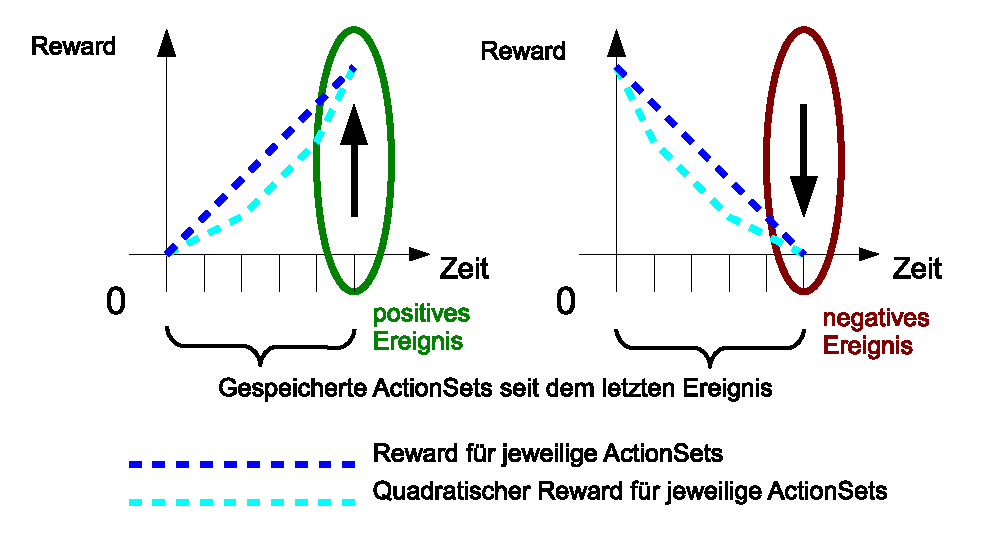
\includegraphics{positive_negative_reward.eps}
}
\caption[Schematische Darstellung der Rewardverteilung an ActionSets] {Schematische Darstellung der (quadratischen) Rewardverteilung an gespeicherte ActionSets bei einem positiven bzw. negativen Ereignis}
\label{positive_negative_reward:fig}
\end{figure}

\subsection{Ereignisse}\label{sec:events}

TODO Anpassen!
In XCS wird lediglich das jeweils letzte ActionSet aus dem vorherigen Zeitschritt gespeichert, in der neuen Implementierung werden dagegen eine ganze Anzahl (bis zu ``maxStackSize'') von ActionSets gespeichert. Die Speicherung erlaubt zum einen eine Vorverarbeitung des Rewards anhand der vergangenen Zeitschritte und auf Basis einer gr��eren Zahl von ActionSets und zum anderen die zeitliche Relativierung eines ActionSets zu einem Ereignis. Die Classifier wird dann jeweils r�ckwirkend anhand des Rewards aktualisiert sobald bestimmte Bedingungen eingetreten sind. 

Von einem positiven bzw. negativen Ereignis spricht man, wenn sich der Reward im Vergleich zum vorangegangenen Zeitschritt ver�ndert hat, also wenn der Zielagent sich in �bertragungsreichweite bzw. aus ihr heraus bewegt hat (siehe ~(\ref{saved_rewards:fig})).

Bei der Benutzung eines solchen Stacks entsteht eine Zeitverz�gerung, d.h. die Classifier besitzen jeweils Information die bis zu ``maxStackSize'' Schritte zu alt sind. W�hlen wir den Stack zu gro�, nimmt die Konvergenzgeschwindigkeit und Reaktionsf�higkeit des Systems zu stark ab, w�hlen wir ihn zu klein, kann es sein, dass wir einen �berlauf bekommen, also ``maxStackSize'' Schritte lang keine Reward�nderung aufgetreten ist. Im letzteren Fall brechen wir deswegen ab,  bewerten die ActionSets der ersten H�lfte des Stacks (also die \(\frac{maxStackSize}{2}\) �ltesten Eintr�ge) mit dem damals vergebenem konstanten Reward (welcher dem aktuellen Reward entspricht, es ist ja keine Reward�nderung eingetreten) und nehmen sie vom Stack (siehe ~(\ref{neutral_reward:fig})). Anschlie�end wird normal weiter verfahren bis der Stack wieder voll ist bzw. bis eine Reward�nderung auftritt. 
Das Szenario mit dem maximalen Fehler w�re das, bei dem ein Schritt nach des Abbruchs eine Reward�nderung auftritt. ``maxStackSize'' stellt also einen Kompromiss zwischen Zeitverz�gerung bzw. Reaktionsgeschwindigkeit und Genauigkeit dar.

\begin{figure}[H]
\setbox0\vbox{\small
Ein Ereignis tritt auf, wenn:
\begin{enumerate}
\item Positive Reward�nderung (Zielagent war im letzten Zeitschritt nicht in �berwachungsreichweite) \(\Rightarrow\) positives Ereignis (mit reward = \(1\))
\item Negative Reward�nderung (Zielagent war im letzten Zeitschritt in �berwachungsreichweite) \(\Rightarrow\) negatives Ereignis (mit reward = \(0\))
\item �berlauf des Stacks (keine Reward�nderung in den letzten ``maxStackSize'' Schritten), Zielagent ist in �berwachungsreichweite \(\Rightarrow\) neutrales Ereignis (mit reward = \(1\))
\item �berlauf des Stacks (keine Reward�nderung in den letzten ``maxStackSize'' Schritten), Zielagent ist nicht in �berwachungsreichweite \(\Rightarrow\) neutrales Ereignis (mit reward = \(0\))
\end{enumerate}
}
\centerline{\fbox{\box0}}
\end{figure}

\begin{figure}[htbp]
\centerline{	
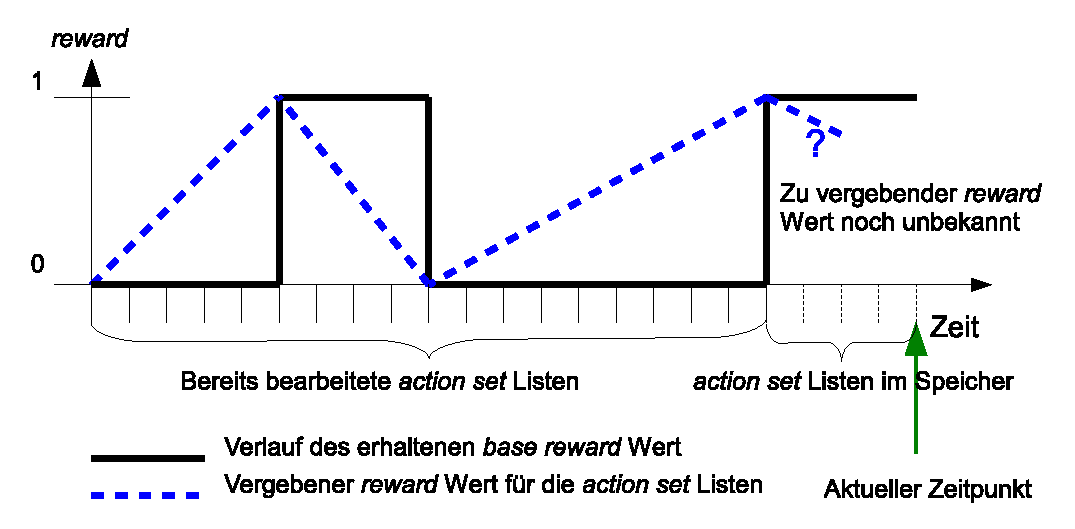
\includegraphics{saved_rewards.eps}
}
\caption[Schematische Darstellung der zeitlichen Rewardverteilung an und der Speicherung von ActionSets] {Schematische Darstellung der zeitlichen Rewardverteilung an ActionSets nach mehreren positiven und negativen Ereignissen und der Speicherung der letzten ActionSets}
\label{saved_rewards:fig}
\end{figure}

\begin{figure}[htbp]
\centerline{	
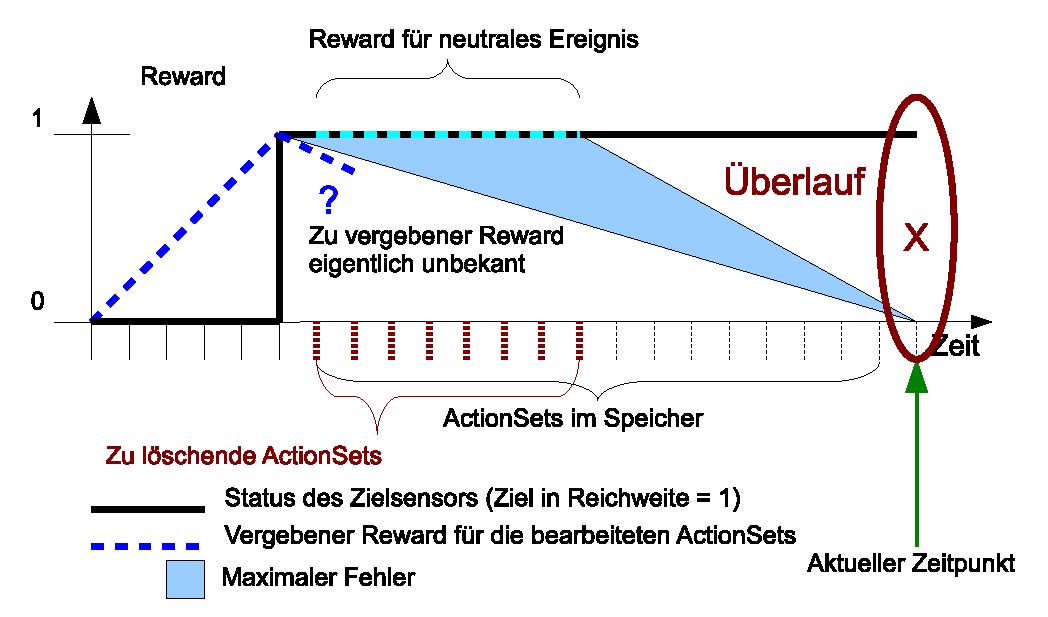
\includegraphics{neutral_reward.eps}
}
\caption[Schematische Darstellung der Rewardverteilung an ActionSets bei einem neutralen Ereignis] {Schematische Darstellung der Rewardverteilung an ActionSets bei einem neutralen Ereignis}
\label{neutral_reward:fig}
\end{figure}

\subsection{Implementierung von SXCS}\label{sxcs_implementation:sec}

TODO Erl�uterung

\begin{program}
  \begin{verbatim}

/**
 * Diese Funktion wird in jedem Schritt aufgerufen um den aktuellen
 * Reward zu bestimmen und positive, negative und neutrale Ereignisse 
 * den besten Wert des ermittelten MatchSets weiterzugeben und, bei 
 * aktuell positivem Reward, das aktuelle ActionSet zu belohnen.
 *
 * @param gaTimestep Der aktuelle Zeitschritt
 */

  public void calculateReward(final long gaTimestep) {
  /**
   * checkRewardPoints liefert "wahr" wenn sich der Zielagent in
   * �berwachungsreichweite befindet
   */
    boolean reward = checkRewardPoints();

    if (reward != lastReward) {
      int start_index = historicActionSet.size() - 1;
      collectReward(start_index, actionSetSize, reward, 1.0, true);
      actionSetSize = 0;
    }
    else 

    if(actionSetSize >= Configuration.getMaxStackSize())
    {
      int start_index = Configuration.getMaxStackSize() / 2;
      int length = actionSetSize - start_index;
      collectReward(start_index, length, reward, 1.0, false);
      actionSetSize = start_index;
    }

    lastReward = reward;
  }
\end{verbatim}
\label{calculateRewardLCS:fig}
  \caption{Erstes Kernst�ck des SXCS-Algorithmus (\emph{calculateReward()}, Bestimmung des Rewards anhand der Sensordaten)}
\end{program}

\begin{program}
  \begin{verbatim}
/**
 * Diese Funktion verarbeitet den �bergebenen Reward und gibt ihn an die
 * zugeh�rigen ActionSets weiter.
 *
 * @param reward Wahr wenn der Zielagent in Sicht war.
 * @param best_value Bester Wert des vorangegangenen ActionSets
 * @param is_event Wahr wenn diese Funktion wegen eines Ereignisses, d.h.
 *        einem positiven Reward, aufgerufen wurde
 */

  public void collectReward(
                boolean reward, double best_value, boolean is_event) {
    double corrected_reward = reward ? 1.0 : 0.0;
  /**
   * Wenn es kein Event ist, dann gebe den Reward weiter wie beim 
   * Multistepverfahren
   */
    double max_prediction = is_event ? 0.0 : 
      historicActionSet.get(start_index+1).getMatchSet().getBestValue();

  /**
   * Aktualisiere eine ganze Anzahl von ActionSets
   */
    for(int i = 0; i < action_set_size; i++) {

  /**
   * Benutze aufsteigenden bzw. absteigenden Reward bei einem positiven 
   * bzw. negativen Ereignis
   */
      if(is_event) {
        corrected_reward = reward ? 
          calculateReward(i, action_set_size) : 
          calculateReward(action_set_size - i, action_set_size);
      }
  /**
   * Aktualisiere das ActionSet mit dem bestimmten Reward und
   * gebe bei allen anderen ActionSets den Reward weiter wie 
   * beim Multistepverfahren 
   */
      ActionClassifierSet action_classifier_set = 
        historicActionSet.get(start_index - i);
      action_classifier_set.updateReward(
        corrected_reward, max_prediction, factor);

      max_prediction = 
        action_classifier_set.getMatchSet().getBestValue();
    }

\end{verbatim}
  \caption{Zweites Kernst�ck des SXCS-Algorithmus (\emph{collectReward()} - Verteilung des Rewards auf die ActionSets)}
\end{program}

\begin{program}
  \begin{verbatim}

/**
 * Bestimmt die zum letzten bekannten Status passenden Classifier und
 * w�hlt aus dieser Menge eine Aktion. Au�erdem wird das aktuelle 
 * ActionClassifierSet mithilfe der gew�hlten Aktion ermittelt.
 * Im Vergleich zur originalen Multistepversion wird am Schlu� noch 
 * das ermittelte ActionSet gespeichert.
 *
 * @param gaTimestep Der aktuelle Zeitschritt
 */

  public void calculateNextMove(long gaTimestep) {

 /**
  * �berdecke das classifierSet mit zum Status passenden Classifiern
  * welche insgesamt alle m�glichen Aktionen abdecken.
  */
    classifierSet.coverAllValidActions(
                    lastState, getPosition(), gaTimestep);

 /**
  * Bestimme alle zum Status passenden Classifier.
  */
    lastMatchSet = new AppliedClassifierSet(lastState, classifierSet);

 /**
  * Entscheide auf welche Weise die Aktion ausgew�hlt werden soll,
  * w�hle Aktion und bestimme zugeh�riges ActionSet
  */
    lastExplore = checkIfExplore(lastState.getSensorGoalAgent(),
                                           lastExplore, gaTimestep);

    calculatedAction = lastMatchSet.chooseAbsoluteDirection(lastExplore);
    lastActionSet = new ActionClassifierSet(lastState, lastMatchSet,
                                                      calculatedAction);

 /**
  * Speichere das ActionSet und passe den Stack bei einem �berlauf an
  */
    actionSetSize++;
    historicActionSet.addLast(lastActionSet);
    if (historicActionSet.size() > Configuration.getMaxStackSize()) {
      historicActionSet.removeFirst();
    }
  }
\end{verbatim}
  \caption{Drittes Kernst�ck des SXCS-Algorithmus (\emph{calculateNextMove()} - Auswahl der n�chsten Aktion und Ermittlung und Speicherung des zugeh�rigen ActionSets)}
\end{program}



\subsection{Zielobjekt mit SXCS}

Wie bereits in Kapitel~\ref{zielobjekt_sxcs_einfuehrung:sec} erw�hnt, soll hier eine Implementierung von SXCS f�r das Zielobjekt diskutiert werden. Bis auf die Funktion \emph{checkRewardPoints()} (siehe Programm~\ref{bewertung:sec}) ist die Implementierung f�r das Zielobjekt identisch. Die abge�nderte Version ist in Programm~\ref{goal_checkRewardPoints:fig} aufgelistet.

\begin{program}
  \begin{verbatim}
    /**
     * @return true Falls das Zielobjekt von keinem Agenten �berwacht wird
     */
    @Override
    public boolean checkRewardPoints() {
      boolean[] sensor_agent = lastState.getSensorAgent();

      for(int i = 0; i < Action.MAX_DIRECTIONS; i++) {
        if(sensor_agent[2*i+1]) {
          return false;
        }
      }

      return true;
    }    \end{verbatim}
  \label{goal_checkRewardPoints:fig}
  \caption{Bestimmung des \emph{base rewards} f�r Agenten}
\end{program}

\section{Unterschiedliche Geschwindigkeiten des Zielobjekts}\label{geschwindigkeit_zielobjekt_xcs:sec}

In Kapitel~\ref{zielgeschwindigkeiten_analyse:sec} wurde dargestellt, dass bis zu einer Geschwindigkeit von 1 die auf Heuristiken basierenden Agenten das Zielobjekt lediglich andauernd verfolgt haben. Bei gr��eren Geschwindigkeiten wurde ein deutlicher Abfall der Qualit�t bemerkt, das Zielobjekt konnte den Agenten also �fters entkommen. Hier werden nun die gleichen Tests f�r lernende Agenten durchgef�hrt.\\

In Abbildung~\ref{goal_agent_speed:fig} ist der Vergleich zwischen XCS und SXCS bez�glich der Qualit�tsdifferenzen bei verschiedenen Geschwindigkeiten des Zielobjekts dargestellt. Neben der von SXCS erreichten im Vergleich zu XCS deutlich h�heren Qualit�tsdifferenz ist hier wie bei den Heuristiken wieder ein Knick zu sehen. Bis zu einer Geschwindigkeit von etwa \(0,7\) bleibt die Qualit�tsifferenz ungef�hr auf einem Niveau um dann abzufallen. Dies zeigt an, dass ein gewisser Teil der erreichten Qualit�t durch eine Strategie der Verfolgung erreicht wurde.\\

\begin{figure}[htbp]
\centerline{	
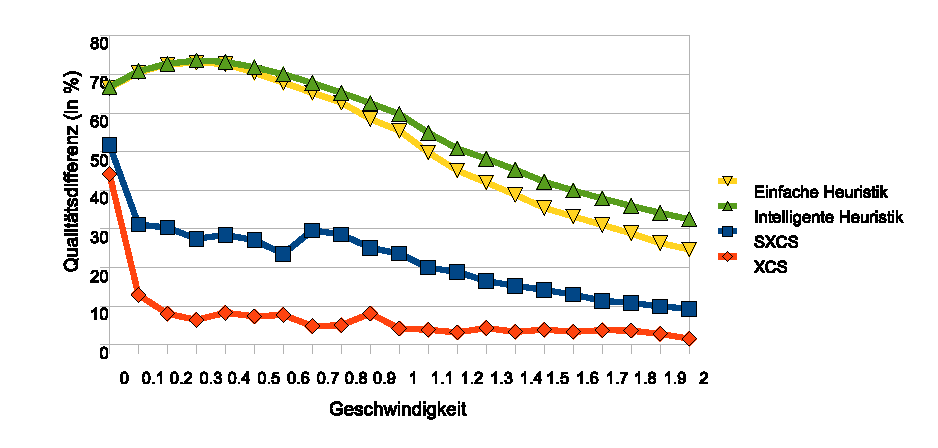
\includegraphics{speed_intelligent_xcs.eps}
}
\caption[Vergleich der Qualit�ten von XCS und SXCS bez�glich der Geschwindigkeit des Zielobjekts] {Vergleich der Qualit�ten von XCS und SXCS bez�glich der Geschwindigkeit des Zielobjekts (intelligentes Zielobjekt, \emph{best selection})}
\label{goal_agent_speed:fig}
\end{figure}


\section{Tests im Szenario mit zuf�llig verteilten Hindernissen}\label{analysis_random_scenario_xcs:sec}

Im vorherigen Abschnitt wurde festgestellt, dass Szenarien mit zuf�llig verteilten Hindernissen (mit \(\lambda_{h} > 0\)) f�r XCS und SXCS eine Herausforderung darstellt. Einfache Tests mit andauernder \emph{exploit} Phase l�sst beide Varianten an dem sehr hohen Anteil an blockierten Bewegungen scheitern. Neben einer Erweiterung der Sensorf�higkeiten und einer Anpassung der \emph{reward} Funktion scheint hier nur ein Wechsel der Auswahlart zur \emph{roulette wheel selection} bzw. der \emph{tournament selection} mit niedrigerem Wert f�r \(p\) Abhilfe zu schaffen. Eine Erh�hung der maximalen Populationsgr��e bringt keine Verbesserung, da die Zahl der neu erstellten \emph{classifier} in einem solchen Szenario nicht viel h�her ist als im S�ulenszenario (siehe Kapitel~\ref{sec:max_population_parameter}).\\

Ein Testlauf mit \emph{roulette wheel selection} erbringt f�r obigen Fall mit Hindernissen und intelligentem Zielobjekt einen �hnlich hohen Wert f�r die Qualit�tsdifferenz (etwa 2,0\%). Eine Verringerung des \emph{tournament factor} Werts mit obiger Konfiguration f�hrt also zu einer Ann�herung der Auswahlart \emph{tournament selection} an die Auswahlart \emph{roulette wheel selection}.\\

Desweiteren ist aufgrund der gro�en Anzahl blockierter Sichtlinien davon auszugehen, dass die Agenten relativ h�ufig keine anderen Agenten in Sicht bekommen, ein \emph{base reward} Wert von \(0\) wird also eher die Seltenheit als die Regel. Zus�tzlich verringert sich dadurch (aus der lokalen Sicht eines Agenten gesehen) die Dynamik des Systems, was die Wiederholung gleicher Aktionen weiter f�rdert. Um dem entgegenzuwirken, wird hier die in Kapitel~\ref{exploreexploit:sec} erw�hnte Auswahlart mit abwechselnder \emph{explore}/\emph{exploit} Phase ausprobiert.\\

Setzt man in der \emph{explore} Phase die Auswahlart \emph{roulette wheel selection} und in der \emph{exploit} Phase die Auswahlart \emph{tournament selection} f�hrt dies zu den Ergebnissen in Abbildung~\ref{vergleich_tournament_factor_roulette:fig}. XCS erreicht auch mit dieser Auswahlart keinen wesentlichen Vorteil gegen�ber dem Algorithmus mit zuf�lliger Bewegung, w�hrend beim SXCS Algorithmus speziell bei \(p = 1,0\), also beim �quivalent zur Auswahlart mit abwechselnder \emph{roulette selection} und \emph{best selection}, ein Ausschlag beim sich intelligent verhaltenden Zielobjekt zu sehen ist. Das Zielobjekt mit einfacher Richtungs�nderung bleibt aber auch hier eine zu schwierige H�rde.\\

\begin{figure}[htbp]
\centerline{	
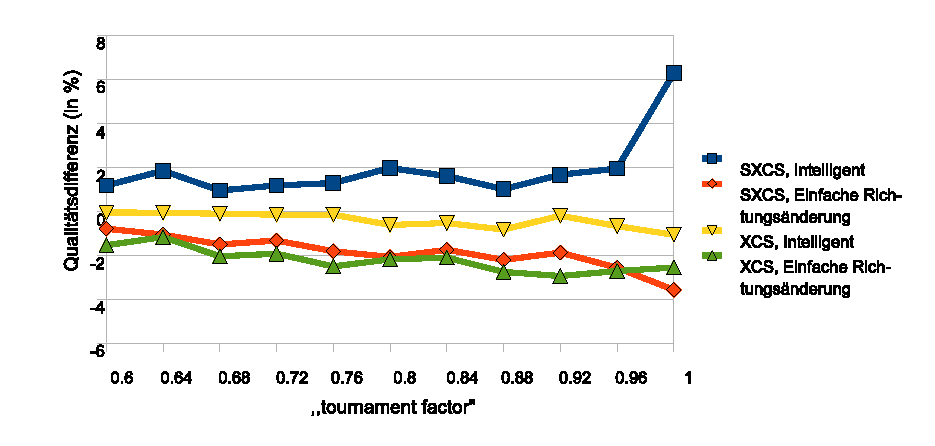
\includegraphics{vergleich_tournament_factor_roulette.eps}
}
\caption[Vergleich verschiedener \emph{tournament factor} Werte bei abwechselnder  \emph{explore}/\emph{exploit} Phase]{Vergleich verschiedener \emph{tournament factor} Werte bei abwechselnder  \emph{explore}/\emph{exploit} Phase (Szenario mit zuf�llig verteilten Hindernissen mit ($\lambda_{p} = 0,99$ und $\lambda_{h} = 0,2$, SXCS Agenten)}
\label{vergleich_tournament_factor_roulette:fig}
\end{figure}

Von den blockierten Bewegungen her konnte mit dieser Auswahlart einerseits die Zahl der blockierten Bewegungen reduziert (auf etwa 34\%) bei XCS  und andererseits weiterhin die M�glichkeit offen gelassen, das Ziel zu verfolgen, wenn es in Sicht ist.\\

Insgesamt ist also zusammenzufassen, dass f�r ein Szenario mit wenigen Hindernissen die Auswahlart \emph{best selection} die beste Wahl ist und in Szenarien mit vielen Hindernissen ein Wechsel der \emph{roulette wheel selection} und \emph{best selection} Auswahlart die beste Wahl ist.\\

Desweiteren war zu sehen, dass hier eindeutig das Szenario mit einem Zielobjekt mit einfacher Richtungs�nderung zu schwierig f�r die betrachteten Agenten. Zwar erreichen die Agenten h�here Werte als im Fall mit intelligenter Heuristik, jedoch ist auch die Qualit�t des zuf�lligen Algorithmus deutlich h�her. Insbesondere besitzen beide Zielobjekttypen die F�higkeit, Hindernisse zu erkennen, d.h. sie bleiben deutlich weniger oft stehen und k�nnen somit schneller aus der Reichweite der Agenten fliehen.\\

W�rde man, wie im Ausblick in Kapitel~\ref{verbesserung_sensoren:sec} erw�hnt, die Sensorf�higkeiten der Agenten und die \emph{reward} Funktion auf Hindernisse erweitern, w�rden sich in diesem Szenario wom�glich Verbesserungen ergeben. Dann w�re es auch m�glich, im Szenario mit vielen Hindernissen die Auswahlart \emph{best selection} zu verwenden. Hierzu m�ssten z.B. Strafen f�r Aktionen verteilt werden. Da die \emph{reward} Funktion eigentlich nur Situationen und nicht Aktionen bewertet, ist eine Analyse der bisher gespeicherten \emph{action set} Listen n�tig. Zeigt der in einer \emph{action set} Liste gespeicherte Sensorstatus ein Hindernis in unmittelbarer N�he an und zeigt die gespeicherte Aktion in die Richtung des Hindernis, k�nnte dies mit einem \emph{base reward} Wert von 0 bewertet werden. Wie bei jeder zus�tzlichen Heuristik muss man sich aber die Frage stellen, wie allgemeing�ltig Agenten mit solchen Modifikationen dann noch agieren k�nnen und ob dadurch nicht optimale L�sungen wegfallen.\\


\subsection{XCS, SXCS und DSXCS im schwierigen Szenario}\label{xcs_difficult_scenario:sec}

Im schwierigen Szenario wurde in Kapitel~\ref{test_schwieriges_szenario:sec} gezeigt, dass hier sich zuf�llige bewegende Agenten wie auch Agenten mit einfacher Heuristik versagen. Auch wurde argumentiert, dass Agenten mit intelligenter Heuristik nur deshalb Erfolg haben, weil sie sich gegenseitig durch die �ffnungen "`dr�ngen"'. Hier werden nun lernende Agenten ihre F�higkeiten unter Beweis stellen. Der wesentliche Vorteil der lernenden Agenten in diesem Szenario ist, dass sie ihr Gelerntes �ber die, wie bisher, 10 Probleminstanzen behalten k�nnen und somit direkt auf den letzten Abschnitt durch die �ffnungen laufen k�nnen, sofern sie das Richtige gelernt haben.\\

Auch wird sich hier wieder das Zielobjekt nur in einer Linie bewegen (siehe Kapitel~\ref{no_direction_change:sec}), es ist also im Grunde kein �berwachungsszenario im eigentlichen Sinne. Wenn ein Agent den letzten Abschnitt auf der rechten Seite erreicht, ist das Problem im Grunde schon gel�st. Prim�r soll, im Vergleich z.B. zum S�ulenszenario, auch gezeigt werden, dass SXCS bei einer solchen Problemstellung im Vergleich zu XCS nicht versagt, also durch die Ab�nderungen nicht die Eigenschaften verliert, die XCS in einfacheren, statischen Problemen zeigt.\\

Zuerst wird mit der einfachen Auswahlart \emph{roulette wheel selection} die Lernrate in Abbildung~\ref{difficult_roulette_learn:fig} getestet. Hier sieht man mehrere Eigenschaften: 

\begin{itemize}
\item SXCS und DSXCS haben in etwa denselben Verlauf.
\item XCS liegt unter der Qualit�t von SXCS.
\item XCS erreicht etwas stabilere Ergebnisse, sichtbar an der glatteren Kurve.
\item F�r SXCS und DSXCS �ndert sich im betrachteten Bereich f�r etwa \(\beta > 0,2\) nichts mehr, f�r XCS f�r etwa \(\beta > 0,7\).
\end{itemize}

\begin{figure}[htbp]
\centerline{	
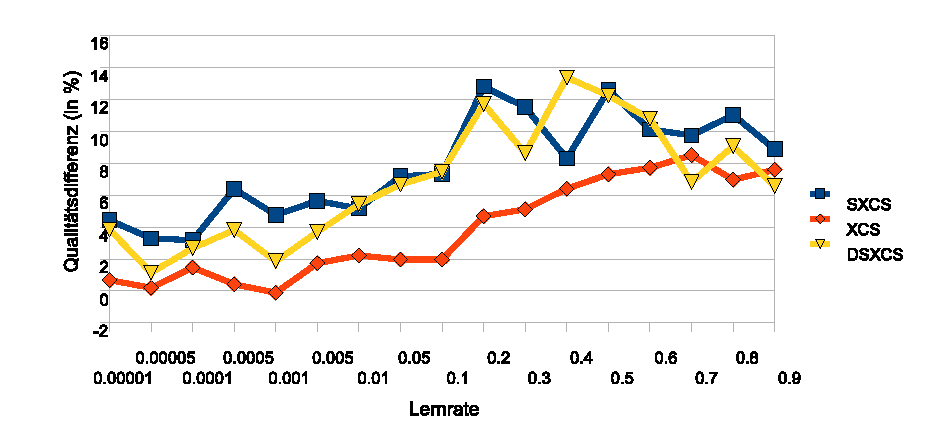
\includegraphics{difficult_roulette_learn.eps}
}
\caption[Auswirkung der Lernrate auf die Qualit�t (schwieriges Szenario) von Agenten mit XCS, SXCS und DSXCS]{Auswirkung der Lernrate auf die Qualit�t (schwieriges Szenario, Agenten mit XCS, SXCS und DSXCS, \emph{roulette wheel selection})}
\label{difficult_roulette_learn:fig}
\end{figure}

Zwar erreicht XCS �hnliche Ergebnisse wie SXCS, allerdings nur durch �ber eine hohe Lernrate. Wie in Kapitel~\ref{sec:learnrate_parameter} gesehen, f�hrt dies aber zu deutlich schlechteren Ergebnissen in anderen Szenarien, weshalb insgesamt gesagt werden muss, dass f�r die benutzte Auswahlart XCS auch hier unterliegt. Insgesamt erscheint \(0,2\) als passender Wert f�r die Lernrate, auch im Hinblick auf die Standardwerte in der Literatur (siehe Kapitel~\ref{uebersicht_parameter:sec}) und bez�glich der Vergleichbarkeit mit Ergebnissen in anderen Szenarien.\\



\subsection{SXCS mit intelligenter Heuristik im schwierigen Szenario}\label{sxcs_intelligent_difficult_test:sec}

Betrachtet man die Ergebnisse der Heuristiken im schwierigen Szenario (siehe Kapitel~\ref{test_schwieriges_szenario:sec}), stellt man fest, dass diese etwas niedriger sind. SXCS hat im betrachteten Szenario in Kapitel~\ref{xcs_difficult_scenario:sec} etwa \(29,24\%\), w�hrend die intelligente Heuristik dort einen Wert von etwa \(40,63\%\) erreicht. Im Folgenden wird nun gepr�ft werden, ob anhand der besprochenen Methoden eine Verbesserung erzielt werden kann.\\

Anstatt \emph{roulette wheel selection} soll nun verst�rkt die Verfahren der \emph{exploit} Phase angewendet werden. Hierzu wurden eine Reihe von Experimenten durchgef�hrt, die erfolgreichsten Ergebnisse erbrachte zuerst eine abwechselnde \emph{explore}/\emph{exploit} Phase mit \emph{roulette wheel selection} und \emph{best selection} mit \(36,22\%\) f�r SXCS (mit \(\beta = 0,2\)), w�hrend sich der XCS Wert nur minimal verbesserte.\\

Noch weiter konnte die Qualit�t durch die Verwendung einer abwechselnden \emph{explore}/\emph{exploit} Phase (mit \emph{tournament selection} in der \emph{explore} Phase und \emph{best selection} in der \emph{exploit} Phase) gesteigert werden (siehe Abbildung~\ref{difficult_roulette_learn2:fig}, die Tests f�r SXCS wurden hier zur Sicherheit �ber 20 Experimente durchgef�hrt). Der hier ermittelte Optimalwert f�r \(p = 0,84\) liegt nun mit 43,75\% (bei \(\beta = 0,2\)) deutlich �ber dem Wert der Heuristik.  Damit ist gezeigt, dass die Quelle der Steigerung aus zus�tzlicher Erlernung der Hindernisse r�hrt, eine Eigenschaft, die der intelligenten Heuristik fehlt.\\

\begin{figure}[htbp]
\centerline{	
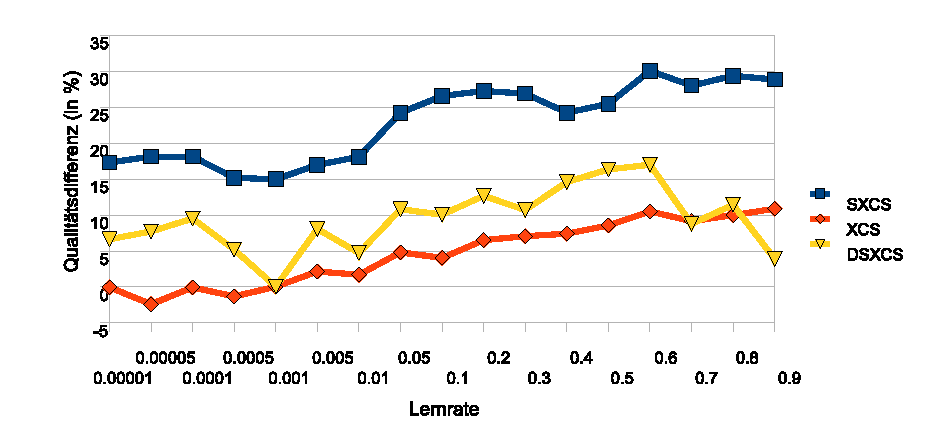
\includegraphics{difficult_roulette_learn2.eps}
}
\caption[Auswirkung der Lernrate auf die Qualit�t (schwieriges Szenario) von Agenten mit XCS und SXCS mit abwechselnder \emph{explore}/\emph{exploit} Phase]{Auswirkung der Lernrate auf die Qualit�t (schwieriges Szenario, Agenten mit XCS und SXCS, mit abwechselnder \emph{explore}/\emph{exploit} Phase)}
\label{difficult_roulette_learn2:fig}
\end{figure}


Als letztes wird eine Variation der Anzahl der Probleminstanzen in Verbindung mit dem schwierigen Szenario betrachtet. Es wird Testlauf durchgef�hrt, bei dem insgesamt jeweils genau 8.000 Schritte durchgef�hrt werden. Die 8.000 Schritte werden allerdings jeweils auf eine unterschiedliche Anzahl von Problemeninstanzen verteilt, d.h. es wird eine Probleminstanz mit 8.000 Schritten, 2 Probleminstanzen mit jeweils 4.000 Schritten, 4 Probleminstanzen mit jeweils 2.000 Schritten usw. getestet. Neben den oben ermittelten Werten f�r die Lernrate \(\beta = 0,2\) und dem Standardwert \emph{tournament factor p}~\( = 0,84\) ist au�erdem (wie in Kapitel~\ref{groesse_stack:sec} untersucht) die Gr��e des Stacks von \(32\) statt \(8\) benutzt worden, was zu einer weiteren Erh�hung der Qualit�t f�hrte.\\

In Abbildung~\ref{difficult_intelligent_sxcs:fig} ist ein Vergleich mit der intelligenten Heuristik dargestellt. Hier sieht man, dass ab 8 Probleminstanzen mit jeweils 500 Schritten der SXCS Algorithmus etwas besser abschneidet als der intelligente Algorithmus. SXCS kann die geringere Schrittzahl durch eine erh�hte Anzahl von Probleminstanzen also durch Erlernen eines Weges durch das Szenario kompensieren. Auch sieht man, dass SXCS bei nur einer Problemzahl eine deutlich niedrigere Qualit�t erreicht. Dies r�hrt daher, dass der Weg zum Ziel bis dahin noch nicht gefunden wurde und erst gelernt werden muss, dann aber bis 8 Probleminstanzen mit der intelligenten Heuristik mith�lt und dann aufgrund der niedrigen Zahl von Schritten abf�llt. Dagegen bedarf XCS ganzer 8 Probleminstanzen um das Maximum zu erreichen, die Lerngeschwindigkeit ist also deutlich geringer.\\

\begin{figure}[htbp]
\centerline{	
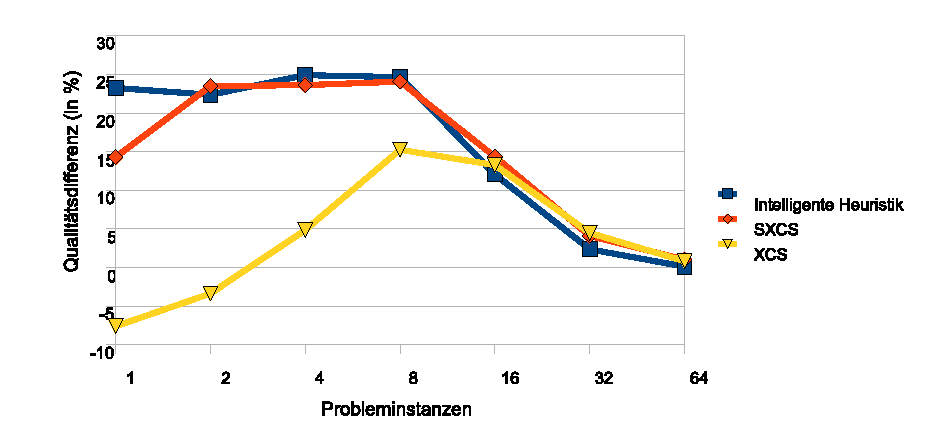
\includegraphics{difficult_intelligent_sxcs.eps}
}
\caption[Qualit�t bei unterschiedlicher Anzahl von Problemen bei gleichbleibender Gesamtzeit (schwieriges Szenario)]{Qualit�t bei unterschiedlicher Anzahl von Problemen bei gleichbleibender Gesamtzeit (schwieriges Szenario)}
\label{difficult_intelligent_sxcs:fig}
\end{figure}



\section{Vergleich SXCS mit DSXCS}\label{dsxcs_analysis:sec}

Wie in Tabelle~\ref{table:dsxcs_comp} zu sehen, erreicht DSXCS im S�ulenszenario mit und ohne Kommunikation nicht die Qualit�t von SXCS. Anzumerken ist allerdings, dass die egoistische Kommunikationsgruppe einen etwas h�heren Wert als die einzelne Kommunikationsgruppe erreicht, was vielleicht bedeutet, dass die Annahme, dass die indiskriminierende Verteilung des \emph{reward} Werts an alle Agenten nachteilig sein k�nnte. Desweiteren f�llt deutlich der Unterschied in der Varianz der Punkte auf, d.h. im Gegensatz zu SXCS �hnelt sich der Anteil, den jeder Agent am Gesamtergebnis beitr�gt, bei den Varianten mit Kommunikation st�rker. Dies wiederum k�nnte auf eine Form kollaborativer Zusammenarbeit deuten. Der geringe Anteil der Varianz von XCS l�sst sich durch das niedrige Ergebnis erkl�ren.\\

\begin{table}[ht]
\caption{Vergleich von SXCS mit den DSXCS Varianten (S�ulenszenario, \emph{best selection})}
\centering
\begin{tabular}{c c c c}
\hline\hline
Algorithmus & Varianz Punkte & Abdeckung & Qualit�t \\ [0.5ex]
\hline
XCS                              & 53,96 & 69,95\% & 12,41\% \\
SXCS                             & 78,51 & 70,50\% & 19,03\% \\
DSXCS (ohne Kommunikation)       & 72,85 & 70,33\% & 16,96\% \\
Einzelne Kommunikationsgruppe    & 49,73 & 68,45\% & 14,91\% \\
Egoistische Kommunikationsgruppe & 47,70 & 68,39\% & 15,30\% \\ [1ex]
\hline
\end{tabular}
\label{table:dsxcs_comp}
\end{table}

Eine Betrachtung des gleitenden Durchschnitts f�hrt auch zu keinen neuen Erkenntnissen (siehe Abbildung~\ref{vergleich_plot_sxcs_dsxcs:fig}). Die zwei Varianten mit Kommunikation haben einen sehr �hnlichen Verlauf, DSXCS liegt etwas unter SXCS und SXCS erreicht zu jedem Zeitpunkt den h�chsten Wert. Anzumerken sei hier nur die Lernkurve der dargestellten Algorithmen.\\

\begin{figure}[htbp]
\centerline{	
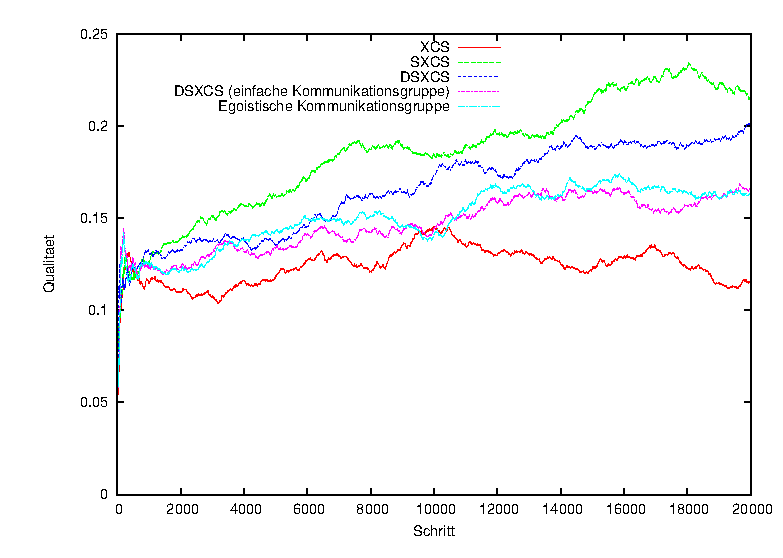
\includegraphics{plot_100_goal_agent_observed-31-03-09--05-20-46-136.eps}
}
\caption[Vergleich des Verlaufs des gleitenden Durchschnitts der Qualit�t von SXCS und DSXCS (S�ulenszenario)]{Vergleich des Verlaufs des gleitenden Durchschnitts der Qualit�t von SXCS und DSXCS (S�ulenszenario, \emph{best selection})}
\label{vergleich_plot_sxcs_dsxcs:fig}
\end{figure}



\section{Bewertung Kommunikation}\label{bewertung_komm:sec}

Bei keiner der zwei in Kapitel~\ref{einfache_gruppe_kommunikation:sec} und Kapitel~\ref{egoistic_relation:sec} vorgestellten Kommunikationsarten konnten in den betrachteten Szenarios Vorteile, was die Qualit�t betrifft, gegen�ber dem SXCS Algorithmus ohne Kommunikation festgestellt werden. Einzig eine etwas h�here Qualit�t der einzelnen Kommunikationsgruppe gegen�ber der DSXCS Variante ohne Kommunikation konnte festgestellt werden.\\

Kommunikation war allerdings nicht der Hauptschwerpunkt dieser Arbeit, die Erweiterung bot sich prim�r an, da sie einfach zu implementieren war. Es ist vor allem in der Theorie mehr Aufwand n�tig um Kommunikation in diesem Zusammenhang zu bewerten. Hinsichtlich der Anzahl m�glicher Erweiterungen, die im Ausblick in Kapitel~\ref{ausblick:sec} aufgelistet sind, erscheint es sinnvoll, den Punkt der Kommunikation in Verbindung mit auf SXCS basierenden Agenten erst wieder aufzugreifen, nachdem diese Punkte untersucht wurden.\\

Die Untersuchung in Kapitel~\ref{dsxcs_analysis:sec} konnte nicht kl�ren, wo das Problem bei dieser Umsetzung von Kommunikation lag. Aufgrund zeitlicher Begrenzung der Arbeit sind die Untersuchungen aber noch nicht abgeschlossen gewesen. Es k�nnen deshalb nur eine Reihe Vermutungen angegeben werden:

\begin{itemize}

\item Die Weitergabe des \emph{reward} Werts basierte auf der Idee, nicht beteiligte Agenten an einem positiven \emph{base reward} zu beteiligen, da sie trotzdem ein Gebiet �berwachen.

\item Die Implementierung �ber den separaten Faktor war nicht zielf�hrend. M�glicherweise muss eine bessere Funktion bei der Auswertung der gespeicherten \emph{action set} Listen gefunden werden (siehe Kapitel~\ref{verzoegerter_reward:sec}).

\item Die Implementierung sorgte bei der Kombination der \emph{reward} Werte bei der egoistischen Kommunikationsgruppe f�r einen unstetige Verlauf der neuen Verteilung des \emph{reward} Werts unter den \emph{action set} Listen (siehe letzter Graph in Abbildung~\ref{corrected_reward:fig}).

\item Die Erwartungen (in Kapitel~\ref{egoistic_relation:sec} an die Agenten, dass sie Gruppen auf Basis des Aktualisierungsfaktors bilden, war zu hoch gegriffen. M�glicherweise muss der Ansatz der �bermittlung der \emph{reward} Werte mittels Aktualisierungsfaktors �berdacht werden.

\item Die indiskriminierende Verteilung des \emph{reward} Werts an alle Agenten sorgte bei der einzelnen Kommunikationsgruppe (siehe Kapitel~\ref{einfache_gruppe_kommunikation:sec}) f�r die Bewertung von Agenten, die nicht zur der L�sung des Problems beigetragen haben.

\item Der relativ geringe Wert f�r die Gr��e des Stacks bei SXCS k�nnte ein Indiz darauf sein, dass nur relativ kurze Wege gelernt werden m�ssen, w�hrend bei der Kommunikation das Augenmerk mehr auf Belohnung l�ngerfristiger Positionierung lag. 

\end{itemize}


\section{Zusammenfassung der Ergebnisse}

In den Tests erreichten die in Kapitel~\ref{analysis_sans_lcs:cha} getesteten Algorithmen mit einfacher und mit intelligenter Heuristik deutlich bessere Werte als die betrachteten XCS Varianten. Dies liegt erst einmal daran, dass das XCS andauernd versucht, mittels genetischer Operatoren neue \emph{classifier} zu generieren, was die Auswahl der Regeln st�ren kann. Auch versuchen die lernenden Agenten andauernd, Korrelationen zu finden, welche nicht unbedingt vorhanden sind. Tritt beispielsweise ein Hindernis gleichzeitig mit dem Zielobjekt auf, so wird das Hindernis (im �bertragenen Sinn) als "`gut"' empfunden, obwohl das Zielobjekt selbst die Hindernisse �berhaupt nicht in die Entscheidung miteinbezieht, in welche Richtung es laufen soll.\\

Schafft man es den in dieser Arbeit vorgestellten SXCS Algorithmus weiter zu verbessern, ist es durchaus denkbar, dass �hnliche Qualit�ten erreicht werden k�nnen. Insbesondere die im Ausblick in Kapitel~\ref{ausblick:sec} diskutierten Erweiterungen bieten sich dazu an.\\

Au�erdem wurde beim Test in Szenarien mit vielen Hindernissen in Kapitel~\ref{analysis_random_scenario_xcs:sec} festgestellt, dass ein hoher Anteil von \emph{exploit} Phasen (bzw. ein gro�er Wert f�r den \emph{tournament factor} \(p\)) dazu f�hren kann, dass einzelne Agenten andauernd in Richtung eines Hindernis laufen. Da dies u.U. zu �ber 70\% blockierten Bewegungen (und entsprechend niedriger Qualit�t) f�hrt, haben die Agenten es also offensichtlich nicht geschafft, Sensorinformationen �ber Hindernisse sinnvoll zu verarbeiten und zu erlernen.\\

Ausnahme hierf�r bieten die Ergebnisse aus dem schwierigen Szenario, der Weg zum Ziel war hier wesentlicher Bestandteil der L�sung, die �ffnungen wurden erkannt und ausgenutzt.\\

Als Gr�nde kann man mehrere Punkte anbringen. Sensorinformationen alleine k�nnen es nicht sein, denn die betrachteten Heuristiken schaffen es schlie�lich v�llig ohne Information �ber die Hindernisse. Aber hier liegt auch schon das, f�r menschliche Beobachter auf den ersten Blick vielleicht etwas seltsam erscheinende, Problem. Ein wesentlicher Punkt ist, dass die Agenten lernen m�ssen, Hindernisse zu ignorieren. Beim gleichzeitigen Auftreten von Hindernissen und dem Zielobjekt ziehen sie u.U. fehlerhafte Schl�sse, da sich das Zielobjekt (fast) unabh�ngig von den Hindernissen bewegt. W�rde sich das Zielobjekt beispielsweise andauernd um eine ganz bestimmte Hinderniskonfiguration herumbewegen, h�tten auf XCS basierende Agenten wohl einen gewissen Vorteil.\\


\chapter{Verz�gertes SXCS}

\section{Verz�gerter Reward}

Der wesentliche Unterschied zur ersten XCS Variante SXCS ist, dass jeglicher ermittelter \emph{reward} Wert und der jeweils zugeh�rige Faktor lediglich zusammen mit den \emph{actionSets} in einer Liste (\emph{historicActionSet} TODO Bezeichnung) gespeichert werden und in jedem Schritt immer nur die \emph{classifiers} des \emph{actionSets} des �ltesten Eintrags in der \emph{historicActionSet} Liste aktualisiert wird. Somit haben wir also eine zeitlich beliebig verz�gerbare Aktualisierungsfunktion, welche uns erlaubt, z.B. gr��ere 

TODO genauer... ist doch sehr �hnlich schon zu dem was wir haben... TODO... beim anderen gibts ja auch Verz�gerung!


Die Funktion \emph{calculateReward} ist identisch mit der in Kapitel ~\ref{calculateRewardLCS:fig}besprochenen Funktion  bei der LCS Variante ohne verz�gerten Reward.

\begin{program}
  \begin{verbatim}
/**
 * Diese Funktion verarbeitet den �bergebenen Reward und gibt ihn an die
 * zugeh�rigen ActionSets weiter. Wesentlicher Unterschied zum LCS ohne 
 * Verz�gerung ist, dass maxPrediction erst bei der endg�ltigen 
 * Verarbeitung des historicActionSets ermittelt wird.
 *
 * @param reward Wahr wenn der Zielagent in Sicht war.
 * @param best_value Bester Wert des vorangegangenen actionSets
 * @param is_event Wahr wenn diese Funktion wegen eines Ereignisses, d.h.
 *        einem positiven Reward, aufgerufen wurde
 */

  public void collectReward(
                boolean reward, double best_value, boolean is_event) {
    double corrected_reward = reward ? 1.0 : 0.0;

  /**
   * Aktualisiere eine ganze Anzahl von Eintr�gen im historicActionSet
   */
     for(int i = 0; i < action_set_size; i++) {

  /**
   * Benutze aufsteigenden bzw. absteigenden Reward bei einem positiven 
   * bzw. negativen Ereignis
   */
       if(is_event) {
         corrected_reward = reward ? 
           calculateReward(i, action_set_size) : 
           calculateReward(action_set_size - i, action_set_size);
       }

  /**
   * F�ge den ermittelten Reward zum historicActionSet
   */
       historicActionSet.get(start_index - i).
         addReward(corrected_reward, factor);

    }

\end{verbatim}
  \caption{Zweites Kernst�ck des verz�gerten LCS-Algorithmus (collectReward - Verteilung des Rewards auf die ActionSets)}
\end{program}

\begin{program}
  \begin{verbatim}

/**
 * Der erste Teil der Funktion ist identisch mit dem calculateNextMove
 * der LCS Variante ohne Kommunikation. Der Zusatz ist, dass beim 
 * �berlauf die im HistoricActionSet gespeicherte Rewards verarbeitet
 * werden
 */

  public void calculateNextMove(long gaTimestep) {
 
  // ... 

  /**
   * HistoryActionSet voll? Dann verarbeite den dort gespeicherten Reward
   */
     if (historicActionSet.size() > Configuration.getMaxStackSize()) {
      HistoryActionClassifierSet first = historicActionSet.pop();
      last.processReward(historicActionSet.getFirst().getBestValue());
    }
  }
\end{verbatim}
  \caption{Auszug aus dem dritten Kernst�ck des verz�gerten LCS-Algorithmus (calculateNextMove)}
\end{program}

\begin{program}
  \begin{verbatim}

/**
 * Zentrale Routine des HistoryActionSets zur Verarbeitung aller 
 * eingegangenen Rewards bis zu diesem Punkt.
 */

  public void processReward(double max_prediction) {

    double max = 0.0;
    double max_factor = 0.0;
  /**
   * Finde das gr��te reward / factor Paar TODO Verbessern
   */
    for(RewardHelper r : reward) {
      if(r.reward >= max && r.factor >= max_factor) {
        max = r.reward;
        max_factor = r.factor;
      }
    }
  /**
   * Aktualisiere den Reward mit den ermittelten Werten und dem
   * �bergebenen maxPrediction Wert
   */
    actionClassifierSet.updateReward(max, max_prediction, max_factor);
  }
\end{verbatim}
  \caption{Auszug aus dem vierten Kernst�ck des verz�gerten LCS-Algorithmus (Verarbeitung des Rewards)}
\end{program}


TODO eigenes Kapitel Kommunikation
\chapter{Kommunikation}\label{communication:cha}

pg. 286 Zentralisierung der Daten

\chapter{LCS mit Kommunikation}

\section{L�sungen aus der Literatur}

Da wir ein Multiagentensystem betrachten, stellt sich nat�rlich die Frage nach der Kommunikation. In der Literatur gibt es Multiagentensysteme die auf Learning Classifier Systemen aufbauen, wie z.B. TODO Literatur. 
Alle Ans�tze in der Literatur erlauben jedoch globale Kommunikation, z.T. Gibt es globale Classifier auf die alle Agenten zur�ckgreifen k�nnen, z.T. gibt es globale Steuerung. 

\cite{Takadama} OCS, centralized control system

In dieser Arbeit betrachte ich das Szenario ohne globale Steuerung oder globale Classifier, also mit der Restriktion einer begrenzten, lokalen Kommunikation.
Geht man davon aus, dass �ber die Zeit hinweg jeder Agent indirekt mit jedem anderen Agenten in Kontakt treten kann, Nachrichten also mit Zeitverz�gerung weitergeleitet werden k�nnen, ist eine Form der globalen, wenn auch zeitverz�gerten, Kommunikation m�glich. TODO 
Eine spezielle Implementierung f�r diesen Fall werde ich weiter unten besprechen TODO

\section{Ablauf}

Jeder Reward, der aus einem normalen Ereignis generiert wird, wird unter Umst�nden an alle anderen Agenten weitergegeben. Wie ein solches sogenanntes ``externes Ereignis'' von diesen Agenten aufgefasst wird, h�ngt von der jeweiligen Kommunikationsvariante ab, die in ~(\ref{sec:kommunikationsvarianten}) besprochen werden.

Durch eine gemeinsame Schnittstelle erh�lt jeder Agent den Reward zusammen mit dem Kommunikationsfaktor. Dabei ergibt sich das Problem, dass sich Rewards �berschneiden k�nnen, da jeder Reward sich r�ckwirkend auf die vergangenen ActionClassifierSets auswirken kann. Auch k�nnen mehrere externe Rewards eintreffen als auch ein eigener lokaler Reward aufgetreten sein. W�rden die Rewards nach ihrer Eingangsreihenfolge abgearbeitet werden, kann es passieren, dass das selbe ActionClassifierSet sowohl mit einem hohen als auch einem niedrigen Reward aktualisiert wird. Da das globale Ziel ist, den Zielagenten durch \emph{irgendeinen} Agenten zu �berwachen, ist es in jedem einzelnen Zeitschritt nur relevant, dass ein \emph{einzelner} Agent einen hohen Reward produziert bzw. weitergibt um die eigene Aktion als zielf�hrend zu bewerten.

Befindet sich das Ziel beispielsweise gerade in �berwachungsreichweite mehrerer Agenten und verliert ein anderer Agent das Ziel aus der Sicht, sollte der Agent (und alle anderen Agenten), der das Ziel in Sicht hat, deswegen nicht bestraft werden, da das globale Ziel ja weiterhin erf�llt wurde.



\subsection{F�lle}

In ~(\ref{sec:events}) wurden 4 verschiedene m�gliche Situationen f�r einen einzelnen Agenten dargestellt. In Verbindung mit externen Rewards ergeben sich einige neue Situationen, n�mlich ob sich der Zielagent in �berwachungsreichweite anderer Agenten befindet und wie dies im letzten Zeitschritt ausgesehen hat. Zusammen mit den urspr�nglichen vier M�glichkeiten ergeben sich folgende 16 M�glichkeiten:
Hier die erweiterte �bersicht, welche Arten von Events im Rahmen eines Multiagentensszenarios auftreten k�nnen:

\begin{itemize}
\item 
\item 
\item 
\end{itemize}

TODO nochmal �berlegen...

Ziel befindet sich von anderen Agenten in Sicht:
Time-out (Ziel in Sicht)
Time-out (Ziel nicht in Sicht)

Ziel kommt in Sicht
Ziel verschwindet aus Sicht


Gebe keinen Reward an andere Agenten weiter. Es ist nicht relevant, ob ein Agent das Ziel aus den Augen verliert oder nicht, es ist nur relevant, ob der Zielagent weiterhin von anderen Agenten beobachtet wird.
Ein Sonderfall ist, wenn im vorherigen Schritt der Zielagent nicht in Sichtweite eines anderen Agenten stand, also in diesem Schritt auf einmal mehrere Agenten den Zielagenten sehen k�nnen. In diesem Fall gibt nur der erste Agent den Reward weiter und setzt ein Flag.


Ziel verschwindet aus Sicht
War der Zielagent von keinem anderen Agenten in Sicht, dann hat sich der Zielagent hiermit aus der Sichtweite aller Agenten bewegt. Somit haben alle Agenten versagt und der negative Reward wird weitergegeben.





Selbiges wenn das Ziel in Sicht kommt und von keinem anderen Agenten in Sicht ist. Die Agenten waren offensichtlich erfolgreich und k�nnen belohnt werden.

TODOTODOTODOTODO
Ist kein Event aufgetreten und leeren wir die H�lfte des Stacks ist es nicht sinnvoll, einen 0-Reward weiterzugeben, da zwangsl�ufig immer mehrere Agenten eine l�ngere Zeit den Zielagenten nicht sehen, selbst wenn sie sich optimal verteilen / bewegen. TODO

Dies zeigt auch der Test:
TODO

Ist kein Event aufgetreten und haben wir einen 1-Reward vorliegen, dann stellt sich die Frage, ob bereits andere Agenten diesen Reward weitergereicht haben. Befinden sich andere Agenten in Reichweite soll nur ein Agent den Reward weiterreichen.
TODO Test


\section{Kommunikationsvarianten}
\label{sec:kommunikationsvarianten}

Allen hier vorgestellten Kommunikationsvarianten ist gemeinsam, dass sie einen Kommunikationsfaktor berechnen, nach denen sie den externen Reward, den ihnen ein anderer Agent �bermittelt hat, bewerten. Der Kommunikationsfaktor gewichtet alle Verwendungen des Parameters \(\beta\) (welcher die Lernrate bestimmt). Ein Faktor von \(1.0\) hie�e, dass der externe Reward wie ein normaler Reward behandelt wird, ein Faktor von \(0.0\) hie�e, dass externe Rewards deaktiviert sein sollen.
Die Idee ist, dass unterschiedliche Agenten unterschiedlich stark am Erfolg des anderen Agenten beteiligt sind, da ohne Kommunikation jeder Agent versuchen wird, selbst den Zielagenten m�glichst in die eigene �berwachungsreichweite zu bekommen, anstatt mit anderen Agenten zu kooperieren, also das Gebiet des Grids m�glichst gro�r�umig abzudecken.

\subsection{No external reward}

Mit dieser Variante wird der Kommunikationsfaktor fest auf \(0.0\) gesetzt und Kommunikation ist deaktiviert.

\subsection{Reward all equally}

Mit dieser Variante wird der Kommunikationsfaktor fest auf \(1.0\) gesetzt und es werden alle Rewards in gleicher Weise weitergegeben. Dadurch wird zwischen den Agenten nicht diskriminiert, was letztlich bedeutet, dass zwar zum einen diejenigen Agenten korrekt mit einem externen Reward belohnt werden, die sich zielf�hrend verhalten, aber zum anderen eben auch diejenigen, die es nicht tun. Deren Classifier werden somit zu einem gewissen Grad zuf�llig bewertet, denn es fehlt die Verbindung zwischen Classifier und Reward.
In Tests (TODO) haben sich dennoch in bestimmten F�llen mit ``Reward all equally'' deutlich bessere Ergebnisse gezeigt als im Fall ohne Kommunikation. Dies ist wahrscheinlich darauf zur�ckzuf�hren, dass in diesen F�llen die Kartengr��e und Geschwindigkeit des Zielagenten relativ zur Sichtweite und Lerngeschwindigkeit zu gro� war, die Agenten also annahmen, dass ihr Verhalten schlecht ist, weil sie den Zielagenten relativ selten in Sicht bekamen. Eine Weitergabe des Rewards an alle Agenten kann hier also zu einer Verbesserung f�hren, dabei ist der Punkt aber nicht, dass Informationen ausgetauscht werden, sondern, dass obiges Verh�ltnis zugunsten der Sichtweite gedreht wird. F�r die Auswahl geeigneter Tests sollten die Szenario-Parameter also m�glichst so gew�hlt werden, dass ``Reward all equally'' keinen signifikanten Vorteil gegen�ber ``No external reward'' bringt.
Blickt man auf diesen Sachverhalt aus einer etwas anderen Perspektive ist es auch einleuchtend. Es scheint offensichtlich, dass es relevant ist, ob das Spielfeld z.B. 100x100 oder nur 10x10 Felder gro� ist, wenn es darum geht, das Verhalten �ber die Zeit hinweg zu bewerten. In den Algorithmus f�r die Kommunikation bzw. f�r die Rewardvergabe m�sste man deshalb einen weiteren (festen) Faktor einbauen, der zu Beginn in Abh�ngigkeit von Gr��e des zu �berwachenden Feldes berechnet wird. Dies soll aber nicht Teil der Arbeit werden. TODO



TODO Idee:
Verteilt man den Reward an alle Agenten mit gleichem Faktor heisst das letztlich, dass jeder Agent in jedem Zeitschritt den selben Rewardwert erh�lt. Dann bildet das System der Agenten im Grunde als gemeinsames System von Agenten mit gemeinsamen Sensoren und gemeinsame, ClassifierSet TODO

\subsection{Simple relation}

Eine dritte Implementation vergleicht die Classifier jeweils beider bei der Kommunikation beteiligten Agenten direkt. Alle Classifier des Agenten, der den Reward weitergibt, die ausreichend Erfahrung gesammelt haben und ausreichend genau ist (\emph{experience} und geringes \emph{predictionError}, Bedingung ist identisch mit \emph{isPossibleSubsumer}), werden mit einem identischen Classifier (d.h. mit gleicher \emph{condition} und gleicher \emph{action}) verglichen. Die Differenz der Produkte aus \emph{fitness} und \emph{prediction} geteilt durch den gr��eren \emph{prediction}-Wert der beiden Classifier stellt hier den Faktor dar. 

\emph{pSet1} sei eine Teilmenge (bestehend aus  Classifiern, deren \emph{experience} gr��er als \emph{thetaSubsumer} und dessen \emph{predictionError} kleiner als epsilon0 ist) des ClassifierSets des Agenten, der den Reward vergibt.
\emph{pSet2} sei die gleiche Teilmenge, allerdings des Agenten, der den Reward empf�ngt.

Nun werden Paare identischer Classifier aus \emph{pSet1} und \emph{pSet2} gebildet. Gibt es mehrere Kandidaten f�r den selben Classifier aus \emph{pSet1}, wird der mit dem �hnlichsten Produkt aus \emph{fitness} und \emph{prediction} gew�hlt. Die Differenz zwischen den beiden Classifiern eines jeden Paares wird anhand ihres \emph{prediction}-Werts auf einen Wert zwischen \(0.0\) und \(1.0\) skaliert und aufaddiert. Die resultierende Summe wird schlie�lich durch die Anzahl der Paare dividiert und man erh�lt den Kommunikationsfaktor.

Ein wesentlicher Nachteil hierbei ist nat�rlich, dass Classifier-Daten direkt �bertragen werden m�ssen, was bei gro�er \emph{maxPopulation} u.U. einen hohen Kommunikations- und Speicheraufwand darstellt.

Umgekehrt k�nnte man diese Funktion auch noch ausbauen und weitergehende Vergleiche ausf�hren, auch unter Einbeziehung der restlichen Classifier beider ClassifierSets, deren \emph{condition} bzw. \emph{action} nicht �bereinstimmen. Beispielsweise kann man alle m�glichen Zust�nde der Sensordaten durchgehen, die passenden Classifier beider ClassifierSets ausw�hlen und die Wahrscheinlichkeiten f�r gew�hlte Aktionen vergleichen, was aber hinsichtlich der ben�tigten Rechenzeit nur f�r kleine Mengen von Sensordaten sinnvoll erscheint.

\begin{program}
  \begin{verbatim}
    /**
     * Relation of this classifier set (the active agent classifier set,
     * e.g. the set that received a reward) to another classifier set
     * @param other The other set we want to compare with
     * @return degree of relationship (0.0 - 1.0)
     */
    public double checkDegreeOfRelationship(
                    final MainClassifierSet other) {
        double degree = 0.0;
        int size = 0;
        ArrayList<Classifier> matched = new ArrayList<Classifier>();

        for (Classifier c : getClassifiers()) {
            if(!c.isPossibleSubsumer()) {
                continue;
            }

            Classifier cl = other.getBestIdenticalClassifier(matched, c);
            if (cl != null) {
                matched.add(cl);

                double div = c.getPrediction();
                if(cl.getPrediction() > div) {
                    div = cl.getPrediction();
                }
                if(div != 0.0) {
                    double difference =
                      1.0 - Math.abs(
                        c.getFitness() * c.getPrediction() - 
                        cl.getFitness() * cl.getPrediction()) / div;
                    if(difference > 1.0) {
                        difference = 1.0;
                    } else
                    if(difference < 0.0) {
                        difference = 0.0;
                    }
                    degree += difference;
                }
            }
            size++;
        }

        if(size == 0) {
            return 0.0;
        }

        degree /= (double)size;
\end{verbatim}
  \caption{``Simple relation'', Algorithmus zur Bestimmung des Kommunikationsfaktors basierend auf \emph{prediction} und \emph{fitness} der ClassifierSets}
\end{program}




\subsection{Egoism factor}

Eine weitere Variante berechnet erst einmal f�r jeden Agenten einen ``Egoismus-Faktor'', indem grob die Wahrscheinlichkeit ermittelt wird, dass ein Agent, wenn sich ein anderer Agent in Sicht befindet, sich in diese Richtung bewegt. ``Egoismus''-Faktor, weil ein gro�er Faktor bedeutet, dass der Agent eher einen kleinen Abstand zu anderen Agenten bevorzugt, also wahrscheinlich eher auf eigene Faust versucht, den Zielagenten in Sicht zu bekommen anstatt ein m�glichst gro�es Gebiet abzudecken.\\

Die Hypothese ist, dass Agenten mit �hnlichem Egoismus-Faktor auch einen �hnlichen Classifiersatz besitzen und der Reward nicht an alle Agenten gleichm��ig weitergegeben wird, sondern bevorzugt an �hnliche Agenten. 

Damit g�be es einen Druck in Richtung eines bestimmten Egoismus-Faktors. TODO

Der Vorteil gegen�ber den anderen Verfahren liegt darin, dass der Kommunikationsaufwand hier nur minimal ist, neben dem \emph{reward} muss lediglich der Egoismus Faktor �bertragen und pro Zeitschritt nur einmal berechnet werden.\\
Ein Problem dieser Variante kann sein, dass der Ansatz das Problem selbst schon l�st, indem er kooperatives Verhalten belohnt, unabh�ngig davon, ob Kooperation f�r das Problem sinnvoll ist.

Die Variante m�sste also zum einen in 


schlecht abschneiden TODO


\begin{figure}[htbp]
\centerline{	
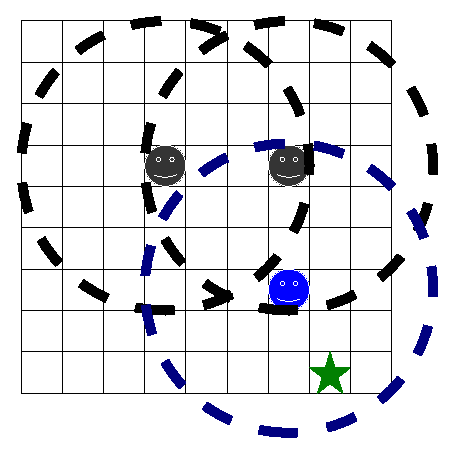
\includegraphics{reward_range.eps}
}
\caption[Schematische Darstellung der Rewardverteilung an ActionSets bei einem neutralen Ereignis] {Schematische Darstellung der Rewardverteilung an ActionSets bei einem neutralen Ereignis}
\label{reward_range:fig}
\end{figure}


\begin{figure}[htbp]
\centerline{	
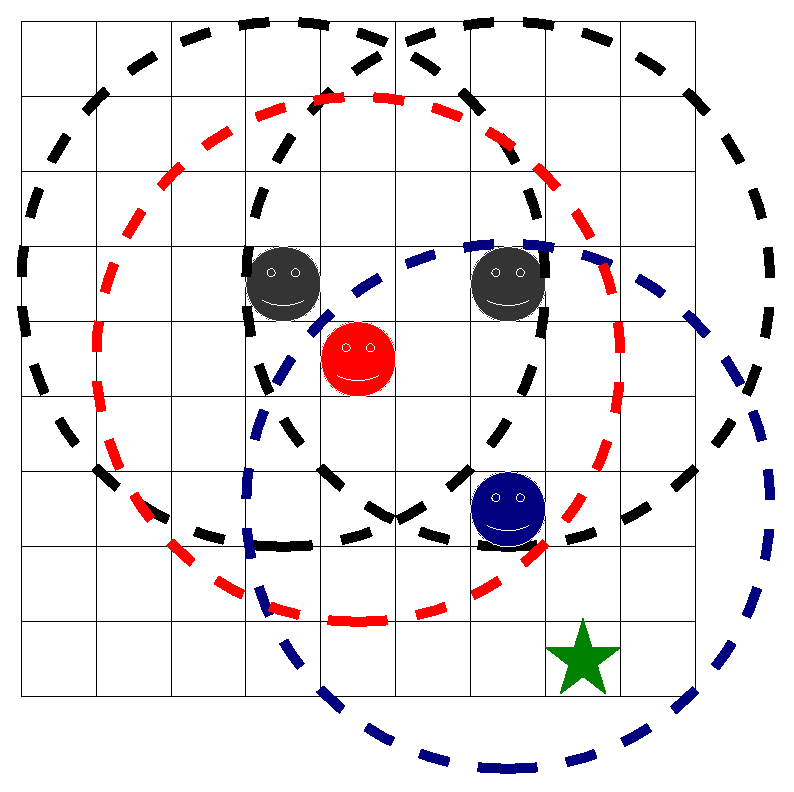
\includegraphics{reward_range_egoist.eps}
}
\caption[Schematische Darstellung der Rewardverteilung an ActionSets bei einem neutralen Ereignis] {Schematische Darstellung der Rewardverteilung an ActionSets bei einem neutralen Ereignis}
\label{reward_range_egoist:fig}
\end{figure}


\begin{figure}[htbp]
\centerline{	
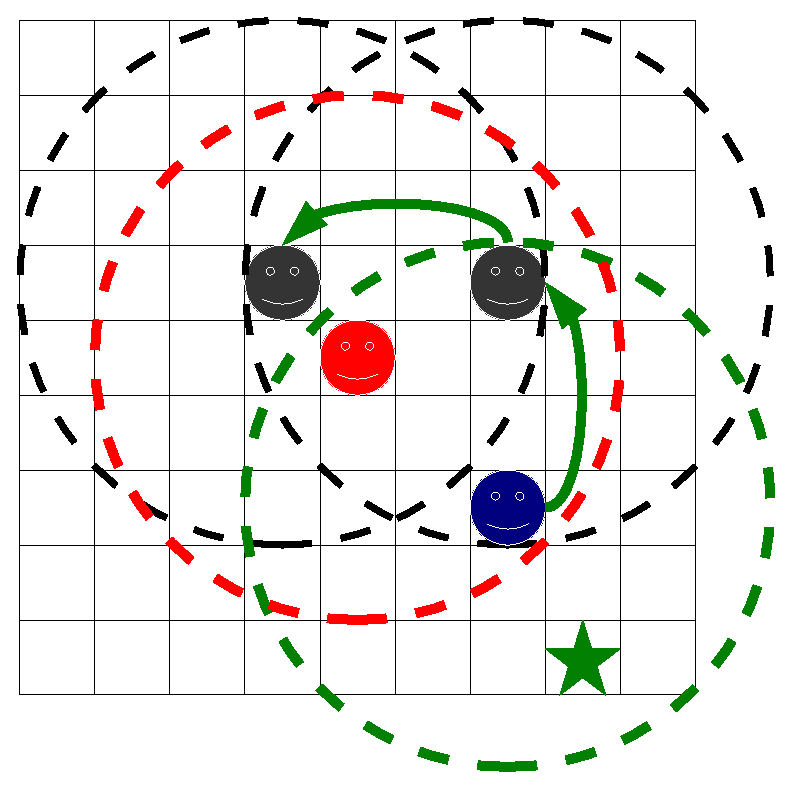
\includegraphics{reward_range_egoist_block.eps}
}
\caption[Schematische Darstellung der Rewardverteilung an ActionSets bei einem neutralen Ereignis] {Schematische Darstellung der Rewardverteilung an ActionSets bei einem neutralen Ereignis}
\label{reward_range_egoist_block:fig}
\end{figure}


\begin{program}
  \begin{verbatim}
    /**
     * Relation of this classifier set (the active agent classifier set,
     * e.g. the set that received a reward) to another classifier set
     * @param other The other set we want to compare with
     * @return degree of relationship (0.0 - 1.0)
     */
    public double checkEgoisticDegreeOfRelationship(
                    final MainClassifierSet other) {
        double ego_factor = 
                 getEgoisticFactor() - other.getEgoisticFactor();
        if(ego_factor == 0.0) {
            return 0.0;
        }
        return 1.0 - ego_factor * ego_factor;
    }

    public double getEgoisticFactor() throws Exception {
        double factor = 0.0;
        double pred_sum = 0.0;
        for(Classifier c : getClassifiers()) {
            if(!c.isPossibleSubsumer()) {
                continue;
            }
            factor += c.getEgoFactor();
            pred_sum += c.getFitness() * c.getPrediction();
        }
        if(pred_sum > 0.0) {
            factor /= pred_sum;
        } else {
            factor = 0.0;
        }
        return factor;
    }
\end{verbatim}
  \caption{``Egoistic relation'', Algorithmus zur Bestimmung des Kommunikationsfaktors basierend auf dem Verhalten des Agenten gegen�ber anderen Agenten}
\end{program}

\section{Realistischer Fall mit Kommunikationsrestriktionen}

Wann immer ein Reward an einen Agenten verteilt wird, kann es sinnvoll sein, diesen Reward an andere Agenten weiterzugeben. Bisher wurde der Fall betrachtet, dass Kommunikation mit beliebiger Reichweite stattfinden kann. Dies ist nat�rlich kein realistisches Szenario. Geht man jedoch davon aus, dass die Kommunikationsreichweite zumindest ausreichend gro� ist um nahe Agenten zu kontaktieren, so kann man argumentieren, dass man dadurch ein Kommunikationsnetzwerk aufbauen kann, in dem jeder Agent jeden anderen Agenten - mit einer gewissen Zeitverz�gerung - erreichen kann. Bei ausreichender Agentenzahl relativ zur freien Fl�che fallen dadurch nur vereinzelte Agenten aus dem Netz, was der Effektivit�t der Agentengruppe erwartungsgem�� nur geringf�gig schadet (TODO zeigen?)
Stehen die Agenten nicht indirekt andauernd miteinander in Kontakt (mit anderen Agenten als Proxy), sondern muss die Information zum Teil durch aktive Bewegungen der Agenten transportiert werden, tritt eine Zeitverz�gerung auf. Auch kann die ben�tigte Bandbreite die verf�gbare �bersteigen, was ebenfalls Zeit ben�tigt.
Im realistischen Fall ist also davon auszugehen, dass jede Kommunikation erst mit einer gewissen Verz�gerung ausgef�hrt wird, weshalb f�r Kommunikation nur der zuvor besprochene verz�gerte LCS Algorithmus in Frage kommt.

TODO lag einf�hren...

\section{Weitergabe des Rewards}

\section{Bewertung Kommunikation:}

Die Vorteile, die man durch Kommunikation erzielen kann, h�ngt stark durch das Szenario ab. Beispielsweise in dem Fall, bei dem zuf�llige Agenten bereits fast 100\% Abdeckung erreichen, also so viele Agenten auf dem Feld sind, dass der Gewinn durch Absprache minimal ist. Auch ist, weil wir nur mit Bin�rsensoren arbeiten, die Sensorik gest�rt, wenn sich sehr viele Agenten auf dem Feld befinden, weil die Sensoren sehr oft gesetzt sind und somit wenig Aussagekraft haben. Erweiterungen wie zus�tzliche Sensoren die die Abst�nde bestimmen w�rde hier wahrscheinlich klarere Ergebnisse liefern.
Umgekehrt ist der Einfluss bei sehr wenigen Agenten gering. TODO

Vergleich unterschiedliche Agentenanzahl, unterschiedliche Kommunikationsmittel
Vergleich mit LCS?

\subsection{Vergleich TODO}

Old LCS Agent
New LCS Agent

Multistep LCS Agent
Dieser Algorithmus stellt eine Implementation des Standard XCS Algorithmus dar. Unterschied zur Standardimplementation ist, dass die Probleminstanz bei Erreichen des tempor�ren Ziels (d.h. den Zielagenten in Sicht zu bekommen) nicht tats�chlich neugestartet wird.
Events, wie bei den neuen LCS Implementationen gibt es nicht, ist das Ziel in Sicht wird Reward 1.0 weitergegeben.

Single LCS Agent

Mehrere LCS Agenten (``Old LCS Agent'') teilen sich ein gemeinsames ClassifierSet, das sie entsprechend updaten.
Entspricht dem Extremfall der Kommunikation
Sight range/Kommunikationsrange





LCS Agenten schneiden auch ohne Kommunikation (bei ausreichender Anzahl von Schritten) immer besser ab als zuf�llige Agenten.

TODOGrafiken



\begin{figure}[htbp]
\centerline{	
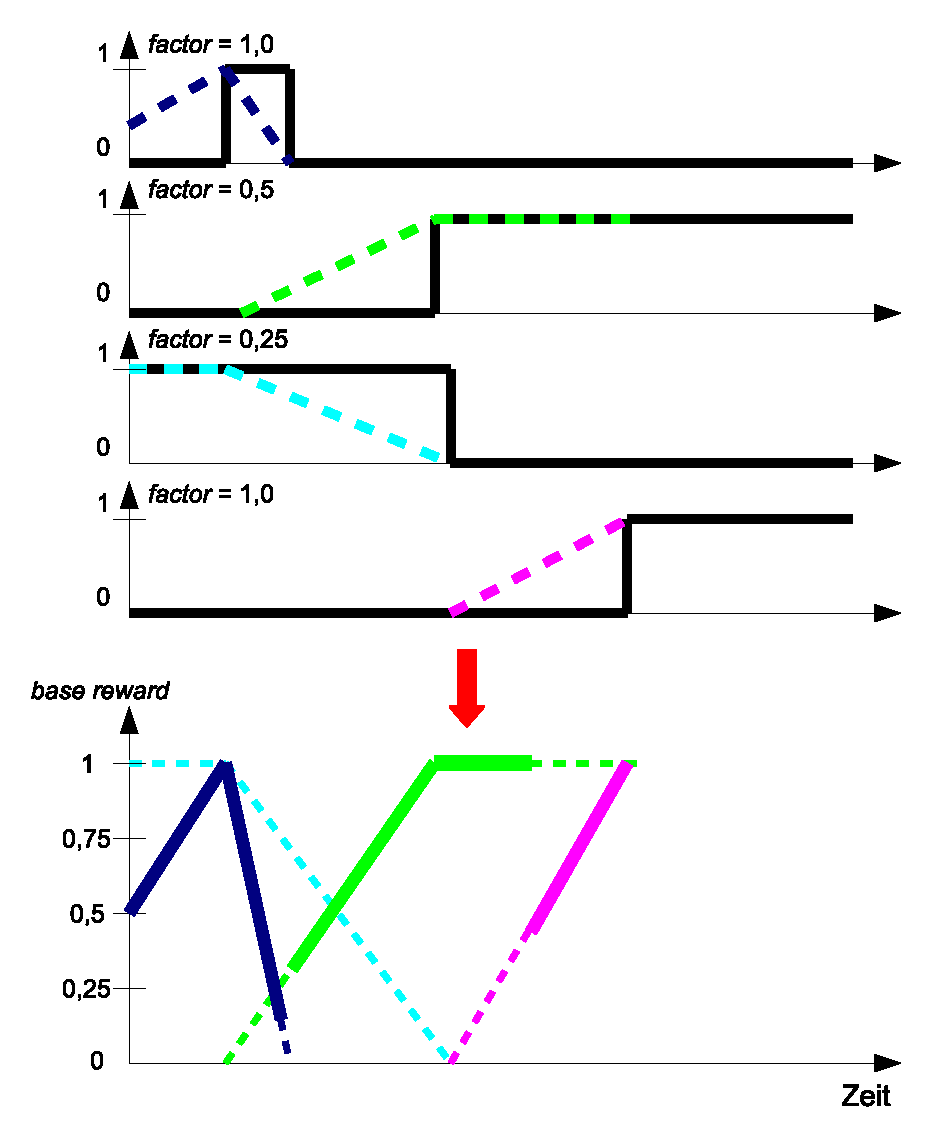
\includegraphics{corrected_reward.eps}
}
\caption[Beispielhafte Darstellung der Kombinierung interner und externer Rewards] {Beispielhafte Darstellung der Kombinierung interner und externer Rewards}
\label{corrected_reward:fig}
\end{figure}


\chapter{Zusammenfassung, Ergebnis und Ausblick}\label{conclusion:cha}


\section{Zusammenfassung}

Zu Beginn wurde auf die Szenariodefinition und die F�higkeiten der Agenten eingegangen. Anhand von Beispielen heuristischer Agenten wurden einige Grundeigenschaften der pr�sentierten Szenarien als Vorbereitung f�r die Analyse der Learning Classifier Systeme bestimmt. Nach der Einf�hrung in LCS, der Beschreibung des Standardverfahren XCS und der angepassten Implementierung f�r �berwachungsszenarios konnten dann umfangreiche Tests ausgef�hrt werden. 


von der M�glichkeit zur Kommunikation eine angepasste Implementierung f�r verz�gerten Reward definiert auf Basis dessen dann mehrere Varianten f�r die Weitergabe des Rewards vorgestellt, analysiert und verglichen wurden.

\section{Ergebnis}
Das wesentliche Ergebnis ist, dass die Implementierung des XCS auf  �berwachungsszenarios ausgeweitet werden kann ohne wesentliche Ver�nderungen am Algorithmus vorzunehmen. W�hrend sich die Qualit�t der resultierenden Agenten im Allgemeinen �ber dem zuf�lligen Agenten befindet, ist die Effizienz der Implementierung, im Vergleich zu einfachen Heuristiken, sehr gering. Mit der verwendeten Implementierung hat XCS Probleme, eine optimale Regelmenge zu finden bzw. zu halten. Eine Regel wie z.B. "`laufe auf das Ziel zu, wenn es in Sicht ist"', ist als Heuristik sehr erfolgreich, bei dauerhafter �berwachung ohne Kommunikation l�uft es aber eher auf ein Verfolgungsszenario hinaus. Aufgrund andauerndem Lernens TODO

Die alleinige Anpassung des XCS Multistepverfahrens, dass ein neues Problem gestartet wird, wann immer sich das Ziel in �berwachungsreichweite befand f�hrte nicht zum Erfolg, die Ergebnisse waren nicht besser als ein sich zuf�llig bewegender Agent.\\


Erst durch Verkn�pfung des Rewards mit dem zeitlichen Abstand zu einer �nderung des Zustands f�hrte zu deutlich besseren Ergebnissen.\\ TODO
Desweiteren wurde untersucht, inwiefern sich der Austausch an minimaler Information unter den Agenten, ohne zentrale Steuerung oder globalem Regeltausch, auf die Qualit�t auswirkt. Zwar gab es vereinzelt positive Effekte, diese waren jedoch auf andere Faktoren zur�ckzuf�hren.



empfindlich gegen�ber Parameter�nderungen

\section{Ausblick}
Ein 


Weitere Untersuchungen sind n�tig um zu bestimmen, inwiefern Kommunikation, beispielsweise mit einer gr��eren Zahl an besseren Sensoren, zu einem besseren Ergebnis f�hren kann. TODO\\
Vom theoretischen Standpunkt ist noch zu kl�ren, warum genau der zeitliche Abstand zum Erfolg gef�hrt hat und wo die Grenzen hierf�r liegen. 

Erschwerung, mehr Kollaboration
TODO aus verschiedenen Richtungen betrachten? Mehrere Agenten notwendig?

Probiert, aber verworfen:

W�hrend der Arbeit wurden auch einige Ans�tze probiert aber mangels Erfolgsaussichten wieder verworfen. Urspr�nglich wurde das Szenario auf Basis von Rotation konzipiert. Die Annahme war, dass ein Agent, der f�r einen Satz an Sensordaten eine optimales \emph{classifier set} gefunden hat, dieses \emph{classifier set} auch f�r Sensordaten eines um 90, 180 und 270 Grad gedrehten Szenarios (mit entsprechend 90, 180 und 270 Grad gedrehter Aktion des jeweiligen \emph{classifier}) optimal sei. Aufgrund der deutlichen Komplexit�tssteigerung des Programms, der niedrigeren Laufzeit und mangels konkreter Qualit�tssteigerungen gegen�ber dem Ansatz ohne Rotation wurde diese Idee jedoch fallengelassen. M�glicherweise k�nnte man durch Hinzunahme eines weiteren Bits im \emph{condition} Vektor, das bestimmt, ob dieser \emph{classifier} gleichzeitig auch die drei rotierten Szenarien erkennen kann, die Leistung des Systems verbessern, dies bedarf aber weiterer Untersuchung und geht am eigentlichen Thema dieser Arbeit vorbei.\\


Abnehmende Exploration LITERATUR
Intelligent Exploration Method to Adapt Exploration Rate in XCS, Based on Adaptive Fuzzy Genetic Algorithm
An Adaptive Approach for the Exploration-Exploitation Dilemma for Learning Agents 

Vielversprechend war anfangs eine Funktion mit der neuerstellte \emph{classifier} mit dem Durchschnittswert aller \emph{reward prediction} Werte einer \emph{classifier set} Liste initialisiert werden. Der Vorteil zeigte sich jedoch nur bei einer zu gering gew�hlten Populationsgr��e (unter 256, siehe Kapitel~\ref{sec:max_population_parameter}), also wenn andauernd neue \emph{classifier} durch \emph{covering} generiert werden m�ssen. Eine weitere Voraussetzung ist, dass sich die \emph{reward prediction} Werte �hneln. Im in dieser Arbeit untersuchten Fall, bei dem die Agenten nur begrenzte Sensorf�higkeiten besitzen, sich auf einem Torus frei bewegen k�nnen.

TODO!

dass sich die \emph{reward prediction} Werte der einzelnen \emph{classifier} untereinander wenig unterscheiden, w�hrend sie beispielsweise bei statischen Szenarien gegen feste, stark unterschiedliche Werte konvergieren. Beispielsweise im Einf�hrungsbeispiel in Abbildung~\ref{simple_scenario_multistep:fig} w�rden die \emph{reward prediction} Werte der \emph{classifier} b), c), e) und g) eher gegen 1 und die der restlichen \emph{classifier} gegen 0 streben.\\
Welchen Wert man f�r \(p_{i}\) nun als Durchschnittswert w�hlt, h�ngt vom jeweiligen Szenario ab. Beispielsweise w�rde ein �berwachungsszenario auf einem sehr gr��eren Torus mit relativ wenigen Agenten w�rde zu einem niedrigeren Durchschnittswert f�r die \emph{reward prediction} Variable f�hren und umgekehrt.\\


In Kapitel TODO wurde eine SXCS Variante vorgestellt, die sowohl mit der Weitergabe des \emph{maxPrediction} wie bei XCS als auch mit der direkten linearen bzw. quadratischen Weitergabe des \emph{base reward} Werts arbeitet. Dadurch ergeben sich Werte f�r den Maximalwert des \emph{reward} \(\rho\) (siehe Kapitel~\ref{epsilon0:sec}) gr��er \(1.0\), womit auch die \emph{reward prediction} Werte der \emph{classifier} aktualisiert werden, wodurch auch diese Werte wiederum gr��er werden, usw. Hier ist noch theoretische Arbeit zu leisten, wie logisch beide Arten der Weitergabe des \emph{reward} sinnvoll miteinander verkn�pft werden k�nnen. In dieser Arbeit konnte nur gezeigt werden, dass in bestimmten Szenarien diese Form der Weitergabe erfolgversprechend ist, wenn es auch f�r einen gewissen Grad der Verf�lschung (und somit auch einer niedrigeren Qualit�t) in Szenarien sorgt, die wenig auf das Erkennen von bestimmten Mustern (wie z.B. beim schwierigen Szenario die �ffnungen) ausgerichtet sind.\\



Sicher interessant ist auch der umgekehrte Ansatz, bei der das Zielobjekt das Objekt ist, das lernt, und den Agenten ausweichen muss. Dieser Aspekt konnte in der Arbeit nur kurz angesprochen werden.\\ TODO



Im Bereich der Kommunikation wurde neben in dieser Arbeit besprochenen "`egoistischen Relation"' (siehe Kapitel~\ref{egoistic_relation:sec}) auch weitere Verfahren ausprobiert, mit welchen versucht wurde, gleichartige Gruppen zu finden. Hier wurden ganze \emph{classifier set} Listen unterschiedlicher Agenten miteinander auf �hnlichkeit gepr�ft um daraus einen Faktor zu berechnen, der (wie bei der "`egoistischen Relation"') Einfluss auf die Weitergabe des \emph{reward} Werts haben sollte. Der dadurch deutlich erh�hte Kommunikations- und Berechnungsaufwand lag jedoch in keinem Verh�ltnis zu eventuell beobachteten Qualit�tsverbesserungen, im Gegenteil wurden eher Qualit�tsverschlechterungen beobachtet. Die Ergebnisse mit dem Test der "`egoistischen Relation"' zeigen jedoch, dass hier zumindest etwas Potential stecken k�nnte und f�r bestimmte Szenarien die zwei Grundideen, dass sich die Agenten zum einen an die Gr��e des Szenarios anpassen und zum anderen der \emph{reward} Wert m�glichst nur an sich �hnlich verhaltende Agenten weitergegeben wird, nicht ganz falsch sein k�nnen. Genauere, insbesondere theoretische, Untersuchungen sind hier n�tig.\\



Was die Szenarien selbst betrifft, wurden ebenfalls mehrere verworfen, da bei ihnen keine zus�tzlichen Beobachtungen gemacht bzw. nur unbedeutende Teilaspekte betrachtet werden konnten. Unter anderem sind dies ein Labyrinth, dessen Umsetzung wahrscheinlich an den mangelnden F�higkeiten der Sensoren scheiterte, ein vereinfachtes "`schwieriges Szenario"' mit einem "`Raum"' mit einer �ffnung in der Mitte, welches sich als zu einfach zu l�sen herausstellte und ein Szenario mit einem Kreuz bestehend aus Hindernissen in der Mitte, welches keine bedeutend anderen Ergebnisse lieferte als das Szenario mit zuf�llig verteilten Hindernissen.\\



\section{Vorgehen und verwendete Hilfsmittel und Software}

Zu Beginn stellte sich die Frage, welche Software zu benutzen ist, da es sich um ein recht komplexe Problemstellung handelt. Begonnen wurde mit der YCS~Implementierung~\cite{Bull03asimple}. Sie ist in der Literatur wenig vertreten, die Implementierung bot aber einen guten Einstieg in das Thema, da sie sich auf das Wesentliche eines LCS beschr�nkte und nur wenige Optimierungen enthielt.\\
Auf Basis des dadurch gewonnenen Wissens war es dann leichter, die XCS Implementierung zu verstehen und nachvollziehen zu k�nnen. Insbesondere die Optimierungen und der etwas unsaubere Programmierstil in der Standardimplementierung bereiteten Probleme.\\

Anhand des Studiums der Literatur war klar, dass in der Richtung der �berwachungsszenarien es wenig Arbeiten, die sich damit besch�ftigten, wie die XCS Implementierung umzusetzen sei. Ein R�ckgriff auf bestehende Bibliotheken war deshalb nicht m�glich, urspr�nglich geplante Untersuchungen komplexerer Systeme wie zentrale Steuerung, Austausch von Regeln etc. wurden gestrichen und es wurde sich auf den einfachen Fall, lokale Information ohne zentrale Steuerung mit h�chstens minimaler Kommunikation beschr�nkt. Dies machte die Verwendung komplexerer Simulationssysteme unn�tig, die Einarbeitungszeit in Multiagenten Frameworks wie z.B. Repast~\cite{repast} erschien zu hoch, wie auch die Risiken, was Geschwindigkeit, Kompatibilit�t und Speicherverbrauch betraf, unbekannt waren, weshalb ein eigenes Simulationsprogramm entwickelt wurde.\\

Das Simulationsprogramm samt zugeh�riger Oberfl�che~\cite{agentsimulator} zur Erstellung von neuen Test-Jobs wurde in Java mit Hilfe von NetBeans~IDE~6.5~\cite{NetBeans} selbst entwickelt und gestaltet.\\

F�r die Verlaufsgraphen wurde GnuPlot~4.2.4~\cite{GnuPlot} benutzt, die Darstellungen der jeweiligen Konfiguration des Torus (insbesondere in Kapitel~\ref{scenario_description:cha}) wurden im Programm mittels Gif89Encoder~\cite{gifencoder} erstellt. Weitere Graphen und Darstellungen wurden OpenOffice.org~Impress und OpenOffice.org~Calc~\cite{OpenOffice} erstellt.\\
Wesentlicher Bestandteil der Konfigurationsoberfl�che war auch eine Automatisierung der Erstellung von Konfigurationsdateien und Batchdateien f�r ein Einzelsystem bzw. f�r JoSchKA~\cite{JoSchKa} zum Testen einer ganzen Reihe von Szenarien und GnuPlot Skripts. Die Automatisierung war aufgrund der tausenden getesteten Szenarien und Parametereinstellungen entscheidend zur Durchf�hrung dieser Arbeit.\\
Dieses Dokument schlie�lich wurde mittels dem \LaTeX Editor LEd 0.5263 \cite{LeD} erstellt und mittels MiKTeX~2.7~\cite{miktex} kompiliert.



\section{Beschreibung des Konfigurationsprogramms}

\begin{figure}[htbp]
\centerline{	
%\includegraphics{agent_configuration.eps}
}
\caption[Screenshot des Konfigurationsprogramms] {Screenshot des Konfigurationsprogramms}
\label{agent_configuration:fig}
\end{figure}




\begin{thebibliography}{99}
\bibitem{Butz} {\sc Butz, M. \& Wilson, S.W.:}  \textit{An Algorithmic Description of XCS}, 2001.
In P-L. Lanzi, W. Stolzmann \& S.W. Wilson (eds) Advances in Learning Classifier Systems: IWLCS 2000. Springer, pp253-272.

\bibitem{Wilson} {\sc Wilson, S.W.:} \textit{Classifier Fitness Based on Accuracy}, 1995
Evolutionary Computation 3(2): 149-175

\bibitem{Butz2000} {\sc Butz, M.:} \textit{XCSJava 1.0: An implementation of the XCS classifier system in Java}
IlliGAL Report No. 2000027, June, 2000
\url{http://www.illigal.uiuc.edu/pub/papers/IlliGALs/2000027.ps.Z}

\bibitem{Bull} {\sc Larry Bull:}  \textit{A Simple Accuracy-Based Learning Classifier System}, 
\url{http://www2.cmp.uea.ac.uk/~it/ycs/ycs.pdf}

\bibitem{Hamer} 
{\sc Carol Hamer}, \textit{J2ME Games With MIDP2}, Apress, 2004,
ISBN 1-590-59382-0
\url{http://www.java-tips.org/java-me-tips/midp/how-to-create-a-maze-game-in-j2me-3.html}

\bibitem{Butz2003} {\sc M. V. Butz, K. Sastry, and D. E. Goldberg:} \textit{�Tournament selection: Stable fitness pressure in XCS,�}
 in Lecture Notes in Computer Science,
E. Cant�-Paz, J. A. Foster, K. Deb, D. Davis, R. Roy, U.-M. O�Reilly,
H.-G. Beyer, R. Standish, G. Kendall, S. Wilson, M. Harman, J.
Wegener, D. Dasgupta, M. A. Potter, A. C. Schultz, K. Dowsland, N.
Jonoska, and J. Miller, Eds. Chicago, IL, Jul. 12�16, 2003, vol. 2724,
Proc. Genetic and Evol. Comput., pp. 1857�1869.

\bibitem{Butz2005} {\sc Martin V. Butz, David E. Goldberg, Pier Luca Lanzi}, \textit{Gradient descent methods in learning classifier systems: Improving XCS performance in multistep problems}
IEEE Transaction on Evolutionary Computation, 9(5):452�473, October 2005.

OCS, Central planning:
\bibitem{Takadama} {\sc Keiki Takadama, Koichiro Hajiri, Tatsuya Nomura, Michio Okada, Shinichi Nakasuka, Katsunori Shimohara} \textit{Learning model for adaptive behaviors as an organized group of swarm robots}
In Artif Life Robotics (1998) 2 : 123-128, ISAROB 1998



\bibitem{Butz2006} {\sc Martin V. Butz} \textit{The XCS Classifier System}
In Studies in Fuzziness and Soft Computing, Springer, 2006, pp51-64.
ISBN 978-3-540-25379-2

\bibitem{Butz2006a} {\sc Martin V. Butz} \textit{Simple Learning Classifier Systems}
In Studies in Fuzziness and Soft Computing, Springer, 2006, pp51-64.
ISBN 978-3-540-25379-2

\bibitem{Wilson1995} {\sc Stewart W. Wilson:} \textit{Classifier Fitness Based on Accuracy}. 
Evolutionary Computation 3(2): 149-175 (1995)


\bibitem{Banzhaf} {\sc W. Banzhaf, J. Daida, A. E. Eiben, M. H. Garzon, V. Honavar, M. Jakiela and R. E. Smith} \textit{�Extending the representation of classifier conditions, Part I: From binary to Messy coding,�}
in Proc. Genetic Evol. Comput. Conf., Eds., 1999b, pp. 337�344.

\bibitem{Barry} {\sc A. M. Barry} \textit{�The stability of long action chains in XCS,�}, 
Soft Comput.�A Fusion Foundations, Methodologies, Applicat., vol. 6, no.
3�4, pp. 183�199, 2002.

\bibitem{xcs1} \textit{�Classifier fitness based on accuracy,�} Evol. Comput., vol. 3,
no. 2, pp. 149�175, 1995

\bibitem{xcs2} {\sc J. R. Koza,W. Banzhaf, K. Chellapilla, K. Deb,
M. Dorigo, D. B. Fogel, M. H. Garzon, D. E. Goldberg, H. Iba, and R.
Riolo} \textit{�Generalization in the XCS classifier system,�}
in Proc. 3rd Ann. Conf. Genetic Program., , Eds., 1998, pp. 665�674.



\bibitem{Lujan} {\sc Alejandro Lujan, Richard Werner, Azzedine Boukerche} \textit{Generation of Rule-based Adaptive Strategies for a
Collaborative Virtual Simulation Environment}
PARADISE Research Laboratory
University of Ottawa TODO
HAVE 2008 � IEEE International Workshop on
Haptic Audio Visual Environments and their Applications
Ottawa � Canada, 18-19 October 2008


Pier Luca Lanzi, Daniele Loiacono, Stewart W. Wilson, and David E.
Goldberg. XCS with Computed Prediction in Continuous Multistep
Environments. In Proceedings of the IEEE Congress on Evolutionary
Computation � CEC-2005, pages 2032�2039, Edinburgh, UK, September
2005. IEEE.


\bibitem{Benouhiba} {\sc Toufik Benouhiba, Jean-Marc Nigro} \textit{An evidential cooperative multi-agent system}
Laboratoire ISTIT, CNRS FRE 2732, Universite� de Technologie de Troyes, Troyes, France

\bibitem{Hiroyashu} {\sc Hiroyasu Inoue, Keiki Takadama, Katsunori Shimohara} \textit{Exploring XCS in Multiagent Environments}

This research was conducted as part of Research on Human
Communication with funding from the National Institute
of Information and Communications Technology.

GECCO 05 June 25.29, 2005, Washington, DC, USA.
Copyright 2005 ACM 1-59593-097-3/05/0006
TODO

\end{thebibliography}


\begin{appendix}
\chapter{Implementation}\label{implementation:cha}

\section{Implementierung eines Problemablaufs}\label{implementierung_ablauf:sec}

In der Schleife der Funktion zur Berechnung eines Experiments (Programm~\ref{mainExperiment:pro}) wird die Funktion zur Berechnung des Problems (\emph{doOneMultiStepProblem()} in Programm~\ref{mainProblem:pro}) aufgerufen. Dort wird in einer weiteren Schleife �ber die Anzahl der maximalen Schritte die Sicht aktualisiert (\emph{updateSight()}), die Qualit�t bestimmt (\emph{updateStatistics()}), die neuen Sensordaten und die n�chste Aktion ermittelt (\emph{calculateAgents()}, siehe Programm~\ref{mainCalculate:pro}), der \emph{reward} Wert ermittelt (\emph{rewardAgents()}, siehe Programm~\ref{mainReward:pro}) und schlie�lich werden die Objekte bewegt (\emph{moveAgents()}, siehe Programm~\ref{mainMove:pro}). Die konkrete Umsetzung der dort aufgerufenen Funktionen (insbesondere \emph{calculateNextMove()} und \emph{calculateReward()}) wird im Kapitel~\ref{lcs_variants:cha} erl�utert (bzw. in Kapitel~\ref{agents:cha}, was die Heuristiken betrifft, wobei \emph{calculateReward()} dort keine Rolle spielt und eine leere Funktion aufgerufen wird).

\newlisting{Zentrale Schleife f�r einzelne Experimente}{mainExperiment:pro}
/**
 * F�hrt eine Anzahl von Problemen aus
 * @param experiment_nr Nummer des auszuf�hrenden Experiments
 */
  public void doOneMultiStepExperiment(int experiment_nr) {
    int currentTimestep = 0;

  /**
   * number of problems for the same population
   */
    for (int i = 0; i < Configuration.getNumberOfProblems(); i++) {

    /**
     * Initialisierung des neuen "Random Seed" Wert
     */
      Misc.initSeed(Configuration.getRandomSeed() + 
        experiment_nr * Configuration.getNumberOfProblems() + i);

    /**
     * Erstellt einen neuen Torus und verteilt Agenten und 
     *   das Zielobjekt neu
     */
      BaseAgent.grid.resetState();

    /**
     * F�hre Problem aus und aktualisiere aktuellen Zeitschritt
     */
      currentTimestep = doOneMultiStepProblem(currentTimestep);
    }
  }
\end{lstlisting}

\newlisting{Zentrale Schleife f�r einzelne Probleme}{mainProblem:pro}
/**
 * F�hrt eine Anzahl von Schritten auf dem aktuellen Torus aus
 * @param stepCounter Aktuelle Zeitschritt
 * @return Der Zeitschritt nach der Ausf�hrung
 */
  private int doOneMultiStepProblem(int stepCounter) {
  /**
   * Zeitpunkt bis zu dem das Problem ausgef�hrt wird
   */
    int steps_next_problem = 
      Configuration.getNumberOfSteps() + stepCounter;    
    for (int currentTimestep = stepCounter; 
         currentTimestep < steps_next_problem; currentTimestep++) {

    /**
     * Ermittle die Sichtbarkeit und erhebe Statistiken
     */
      BaseAgent.grid.updateSight();
      BaseAgent.grid.updateStatistics(currentTimestep);

    /**
     * Ermittle neue Sensordaten und berechne Aktionen der Agenten
     */
      calculateAgents(currentTimestep);

    /**
     * Ermittle den Reward f�r alle Agenten (nach dem ersten Schritt)
     */
      if(currentTimestep > stepCounter) {
        rewardAgents(currentTimestep);
      }

    /**
     * F�hre zuvor berechnete Aktionen aus
     */
      moveAgents();
    }

    /**
     * Abschlie�ende Ermittlung des Rewards
     */
    BaseAgent.grid.updateSight();
    rewardAgents(steps_next_problem);
    return steps_next_problem;
  }
\end{lstlisting}





\newlisting{Zentrale Bearbeitung (Sensordaten und Berechnung der neuen Aktion) aller Agenten und des Zielobjekts innerhalb eines Problems}{mainCalculate:pro}
/**
 * Berechnet die Aktionen und f�hrt sie in zuf�lliger Reihenfolge aus
 * @param gaTimestep der aktuelle Zeitschritt
 */
  private void calculateAgents(final long gaTimestep) {

  /**
   * Ermittle Sensordaten und bestimme n�chste Bewegung
   */
    for(BaseAgent a : agentList) {
      a.aquireNewSensorData();
      a.calculateNextMove(gaTimestep);
    }
    BaseAgent.goalAgent.aquireNewSensorData();
    BaseAgent.goalAgent.calculateNextMove(gaTimestep);
  }
\end{lstlisting}



\newlisting{Zentrale Bearbeitung (Verteilung des \emph{reward} Werts) aller Agenten und des Zielobjekts innerhalb eines Problems}{mainReward:pro}
/**
 * Verteilt den Reward an alle Agenten
 */
  private void rewardAgents(final long gaTimestep) {
    for(BaseAgent a : agentList) {
      a.calculateReward(gaTimestep);
    }
    BaseAgent.goalAgent.calculateReward(gaTimestep);
  }
\end{lstlisting}



\newlisting{Zentrale Bearbeitung (Ausf�hrung der Bewegung) aller Agenten und des Zielobjekts innerhalb eines Problems}{mainMove:pro}
/**
 * Berechnet die Aktionen und f�hrt sie in zuf�lliger Reihenfolge aus
 * @param gaTimestep der aktuelle Zeitschritt
 */
  private void moveAgents(long gaTimestep) {
  /**
   * Erstelle Ausf�hrungsliste f�r alle Objekte (Zielobjekt mehrfach)
   */
    int goal_speed = Configuration.getGoalAgentMovementSpeed();
    ArrayList<BaseAgent> random_list = 
      new ArrayList<BaseAgent>(agentList.size() + goal_speed);

    random_list.addAll(agentList);
    for(int i = 0; i < goal_speed; i++) {
      random_list.add(BaseAgent.goalAgent);
    }

  /**
   * F�hre die ermittelten Aktionen in zuf�lliger Reihenfolge aus
   *   (Zielobjekt kann mehrfach ausgef�hrt werden).
   */
    int[] array = Misc.getRandomArray(random_list.size());
    for(int i = 0; i < array.length; i++) {
      BaseAgent a = random_list.get(array[i]);
      a.doNextMove();
      if(a.isGoalAgent() && goal_speed > 1) {
        goal_speed--;
        a.aquireNewSensorData();
        a.calculateNextMove(gaTimestep);
        a.calculateReward(gaTimestep);
      }
    }
  }
\end{lstlisting}

\clearpage



\section{Typen von Agentenbewegungen}

\newlisting{Berechnung der n�chsten Aktion bei der Benutzung des Algorithmus mit zuf�lliger Bewegung}{calculateNextMoveRandomAlgorithm:pro}
/**
 * Berechne n�chste Aktion (zuf�lliger Algorithmus)
 */
  private void calculateNextMove() {
  /**
   * W�hle zuf�llige Richtung als n�chste Aktion
   */
    calculatedAction = Misc.nextInt(Action.MAX_DIRECTIONS);
  }
\end{lstlisting}


\newlisting{Berechnung der n�chsten Aktion bei der Benutzung der einfachen Heuristik}{calculateNextMove_SimpleHeuristic:pro}
/**
 * Berechne n�chste Aktion (einfache Heuristik)
 */
  private void calculateNextMove() {
  /**
   * Holt sich die Informationen der Gruppe der Sensoren, die auf 
   * das Zielobjekt ausgerichtet sind
   */
    boolean[] goal_sensor = lastState.getSensorGoal();
    calculatedAction = -1;
    for(int i = 0; i < Action.MAX_DIRECTIONS; i++) {
    /**
     * Zielagent in Sicht in dieser Richtung?
     */
      if(goal_sensor[2*i]) {
        calculatedAction = i;
        break;
      }
    }

  /**
   * Sonst w�hle zuf�llige Richtung als n�chste Aktion
   */
    if(calculatedAction == -1) {
      calculatedAction = Misc.nextInt(Action.MAX_DIRECTIONS);
    }      

  }
\end{lstlisting}

\newlisting{Berechnung der n�chsten Aktion bei der Benutzung der intelligenten Heuristik}{calculateNextMove_IntelligentHeuristic:pro}
/**
 * Berechne n�chste Aktion (intelligente Heuristik)
 */
private void calculateNextMove() {
  /**
   * Holt sich die Informationen der Gruppe der Sensoren, die auf 
   * das Zielobjekt ausgerichtet sind
   */
    boolean[] goal_sensor = lastState.getSensorGoal();

    calculatedAction = -1;
    for(int i = 0; i < Action.MAX_DIRECTIONS; i++) {
    /**
     * Zielagent in Sicht in dieser Richtung?
     */
      if(goal_sensor[2*i]) {
        calculatedAction = i;
        break;
      }
    }

  /**
   * Zielobjekt nicht in Sicht? Dann bewege von Agenten weg
   */
    if(calculatedAction == -1) {
      calculatedAction = Misc.nextInt(Action.MAX_DIRECTIONS);

      boolean[] agent_sensors = lastState.getSensorAgent();
      boolean one_free = false;
      for(int i = 0; i < Action.MAX_DIRECTIONS; i++) {
        if(!agent_sensors[2*i]) {
          one_free = true;
          break;
        }
      }

      if(one_free) {
        while(agent_sensors[2*calculatedAction]) {
          calculatedAction = Misc.nextInt(Action.MAX_DIRECTIONS);
        }
      }
    } 
  }
\end{lstlisting}

\clearpage



\section{Korrigierte \emph{addNumerosity()} Funktion}\label{corrected_numerosity_function:sec}

Durch die Benutzung von \emph{macro classifier} ergibt sich das programmiertechnische Problem, dass man nicht mehr direkt wei�, wieviele \emph{micro classifier} sich in einer Population befinden, bei jeder Benutzung des Werts der Populationsgr��e m�ssten die \emph{numerosity} Werte aller \emph{classifier} jedes Mal addiert werden. In der Standardimplementierung \cite{Butz_xcsclassifier} ist die Behandlung des \emph{numerosity} Werts deswegen stark optimiert, jedes \emph{classifier set} tr�gt eine tempor�re Variable \emph{numerositySum} mit sich, in der die aktuelle Summe gespeichert ist. Die Aktualisierung ist jedoch zum einen mangelhaft umgesetzt, zum anderen auf die Verwendung von einer einzelnen \emph{action set} Liste optimiert, w�hrend die hier verwendete Implementierung jeweils mit bis �ber 100 \emph{action set} Listen programmiert wurde, denen ein \emph{classifier} Mitglied sein kann. Deswegen wurde die Optimierung entfernt und durch eine dezentrale Verwaltung mit einem \emph{Observer} ersetzt, jede �nderung des \emph{numerosity} Wertes hat also die �nderung aller \emph{action set} Listen zur Folge, in der der \emph{classifier} Mitglied ist.\\

Wird also z.B. ein \emph{micro classifier} entfernt, dann wird lediglich die �nderungsfunktion des \emph{classifiers} aufgerufen, der dann wiederum den \emph{numerositySum} Wert der jeweiligen Eltern anpasst. Dies macht einige Optimierungen r�ckg�ngig, erspart aber sehr viel Umst�nde, den \emph{numerositySum} der Eltern immer auf den aktuellen Stand zu halten und einzelne \emph{classifiers} zu l�schen.\\

Positiver Nebeneffekt durch die verbesserte Struktur ist, dass man dadurch leicht auf die Menge der \emph{action set} Listen zugreifen kann, denen ein \emph{classifier} angeh�rt, hierf�r wurde aber im Rahmen dieser Arbeit keine Verwendung gefunden.\\

Ein weiteres Problem der Standardimplementierung ist, dass der \emph{fitness} Wert eines \emph{classifiers} als Optimierung bereits den \emph{numerosity} Wert als Faktor enth�lt, w�hrend bei der Aktualisierung des \emph{numerosity} Werts der \emph{fitness} Wert nicht aktualisiert wurde. Das hat zur Folge, dass theoretisch \emph{fitness} Werte von \emph{classifiers} fast den \emph{max population} Wert annehmen kann, wenn ein \emph{classifier} mit \emph{numerosity} und \emph{fitness} Wert in der H�he von \emph{max population} auf einen \emph{numerosity} Wert von \(1,0\) reduziert wird.\\
Dies betrifft die Funktion \emph{public void addNumerosity(int num)} der Klasse \emph{XClassifier} in der Datei \emph{XClassifier.java}. Die Korrektur besteht darin, den \emph{fitness} Wert mit dem Quotienten aus dem neuen durch den alten \emph{numerosity} Wert zu multiplizieren. Die korrigierte Fassung ist in Programm~\ref{corrected_numerosity_function:pro} dargestellt.\\

M�glicherweise kann man diesen Fehler durch Ver�nderung der Parameter oder l�ngere Laufzeiten kompensieren, logisch betrachtet macht es aber keinen Sinn, dass beim Subsummieren bzw. L�schen eines \emph{micro classifier} der \emph{fitness} Wert ver�ndert wird. In Tests haben sich nur minimale Unterschiede ergeben. Beispielsweise ergab sich (auf dem S�ulenszenario mit 8 Agenten mit SXCS und einem Zielobjekt mit einfacher Richtungs�nderung) eine Qualit�t von \(39,15\%\) im Vergleich zur originalen Implementierung von \(39,95\%\) bei 500 Schritten bzw. \(35,42\%\) zu \(35,01\%\) bei 2000 Schritten. Der Fehler scheint sich also eher langfristig auszuwirken, wenn auch der Unterschied so klein ist, dass man ihn vernachl�ssigen kann. Problematisch wird es, wenn Modifikationen von XCS darauf aufbauen, dass der \emph{fitness} Wert f�r jeden \emph{micro classifier} immer kleiner gleich \emph{1.0} ist.\\

Alles in allem betrachtet soll im Rahmen dieser Arbeit soll die korrigierte Fassung benutzt werden.

\newlisting{Korrigierte Version der \emph{addNumerosity()} Funktion}{corrected_numerosity_function:pro}
/**
 * Erh�ht oder erniedrigt den numerosity Wert des classifier
 * @param num Der zur numerosity zu addierende Wert (kann negativ sein).
 */
  public void addNumerosity(int num) {
    int old_num = numerosity;
   
    numerosity += num;

  /**
   * Korrektur der fitness
   */
    if(old_num > 0) {
      fitness = fitness * (double)numerosity / (double)old_num;
    } else {
      fitness = Configuration.
    }

  /**
   * Aktualisierung der Eltern
   */
    for (ClassifierSet p : parents) {
      p.changeNumerositySum(num);
      if (numerosity == 0) {
        p.removeClassifier(this);
      }
    }
  }
\end{lstlisting}


\clearpage

\section{Implementierung XCS Multistepverfahrens }

\newlisting{Erstes Kernst�ck des Standard XCS Multistepverfahrens (\emph{calculateReward()}, Bestimmung und Verarbeitung des \emph{reward} Werts anhand der Sensordaten), angepasst an ein dynamisches �berwachungsszenario, bei positivem \emph{reward} Wert wird nicht abgebrochen}{multistep_calc_reward:pro}
/**
 * Diese Funktion wird in jedem Schritt aufgerufen um den aktuellen
 * reward zu bestimmen, den besten Wert der ermittelten match set Liste
 * weiterzugeben und, bei aktuell positivem reward, die aktuelle
 * action set Liste zu belohnen.
 *
 * @param gaTimestep Der aktuelle Zeitschritt
 */

  public void calculateReward(final long gaTimestep) {
  /**
   * checkRewardPoints liefert "wahr" wenn sich das Zielobjekt in
   * �berwachungsreichweite befindet
   */
    boolean reward = checkRewardPoints();

    if(prevActionSet != null){
      collectReward(lastReward, lastMatchSet.getBestValue(), false);
      prevActionSet.evolutionaryAlgorithm(classifierSet, gaTimestep);
    }

    if(reward) {
      collectReward(reward, 0.0, true);
      lastActionSet.evolutionaryAlgorithm(classifierSet, gaTimestep);
      prevActionSet = null;
      return;
    }
    prevActionSet = lastActionSet;
    lastReward = reward;
  }
\end{lstlisting}


\newlisting{Zweites Kernst�ck des XCS \emph{multi step} Verfahrens (\emph{collectReward()} - Verteilung des \emph{reward} Werts auf die \emph{action set} Listen), angepasst an ein dynamisches �berwachungsszenario}{multistep_collect_reward:pro}
/**
 * Diese Funktion verarbeitet den �bergebenen reward Wert und 
 * gibt ihn an die zugeh�rigen action set Listen weiter.
 *
 * @param reward Wahr wenn das Zielobjekt in Sicht war.
 * @param best_value Bester Wert des vorangegangenen action set Listen
 * @param is_event Wahr wenn diese Funktion wegen eines Ereignisses, 
 *          d.h. einem positiven reward Wert, aufgerufen wurde
 */

  public void collectReward(boolean reward, 
                double best_value, boolean is_event) {
    double corrected_reward = reward ? 1.0 : 0.0;

  /**
   * Falls der reward Wert von einem Ereignis r�hrt, aktualisiere die 
   * aktuelle action set Liste und l�sche das vorherige
   */
    if(is_event) {
      if(lastActionSet != null) {
        lastActionSet.updateReward(corrected_reward, best_value, factor);
        prevActionSet = null;
      }
    } 

  /**
   * Kein Ereignis, also nur die letzte action set Liste aktualisieren
   */
    else 
    {
      if(prevActionSet != null) {
        prevActionSet.updateReward(corrected_reward, best_value, factor);
      }
    }
  }
\end{lstlisting}



\newlisting{Drittes Kernst�ck des XCS \emph{multi step} Verfahrens (\emph{calculateNextMove()}, Auswahl der n�chsten Aktion und Ermittlung der zugeh�rigen \emph{action set} Liste), angepasst an ein dynamisches �berwachungsszenario}{multistep_calc_move:pro}
/**
 * Bestimmt die zum letzten bekannten Status passenden classifier und
 * w�hlt aus dieser Menge eine Aktion. Au�erdem wird die aktuelle 
 * action set Liste mithilfe der gew�hlten Aktion ermittelt.
 *
 * @param gaTimestep Der aktuelle Zeitschritt
 */

  public void calculateNextMove(long gaTimestep) {

 /**
  * �berdecke das classifierSet mit zum Status passenden Classifiern
  * welche insgesamt alle m�glichen Aktionen abdecken.
  */
    classifierSet.coverAllValidActions(
                    lastState, getPosition(), gaTimestep);

 /**
  * Bestimme alle zum Status passenden Classifier.
  */
    lastMatchSet = new AppliedClassifierSet(lastState, classifierSet);

 /**
  * Entscheide auf welche Weise die Aktion ausgew�hlt werden soll.
  */
    lastExplore = checkIfExplore(lastState.getSensorGoalAgent(),
                                           lastExplore, gaTimestep);

 /**
  * W�hle Aktion und bestimme zugeh�rige action set Liste
  */
    calculatedAction = lastMatchSet.chooseAbsoluteDirection(lastExplore);
    lastActionSet = new ActionClassifierSet(lastState, lastMatchSet,
                                                      calculatedAction);
  }
\end{lstlisting}



\clearpage

\section{Implementierung des SXCS Verfahrens}

\newlisting{Erstes Kernst�ck des SXCS-Algorithmus (\emph{calculateReward()}, Bestimmung des Rewards anhand der Sensordaten)}{sxcs_calc_reward:pro}
/**
 * Diese Funktion wird in jedem Schritt aufgerufen um den aktuellen
 * reward Wert zu bestimmen und positive, negative und neutrale 
 * Ereignisse den besten Wert der ermittelten match set Liste 
 * weiterzugeben und, bei aktuell positivem reward Wert, die 
 * aktuelle action set Liste zu belohnen.
 *
 * @param gaTimestep Der aktuelle Zeitschritt
 */

  public void calculateReward(final long gaTimestep) {
  /**
   * checkRewardPoints liefert "wahr" wenn sich der Zielobjekt in
   * �berwachungsreichweite befindet
   */
    boolean reward = checkRewardPoints();

    if (reward != lastReward) {
      int start_index = historicActionSet.size() - 1;
      collectReward(start_index, actionSetSize, reward, 1.0, true);
      actionSetSize = 0;
    }
    else 

    if(actionSetSize >= Configuration.getMaxStackSize())
    {
      int start_index = Configuration.getMaxStackSize() / 2;
      int length = actionSetSize - start_index;
      collectReward(start_index, length, reward, 1.0, false);
      actionSetSize = start_index;
    }

    lastReward = reward;
  }
\end{lstlisting}




\newlisting{Zweites Kernst�ck des SXCS-Algorithmus (\emph{collectReward()} - Verteilung des \emph{reward} Werts auf die \emph{action set} Listen)}{sxcs_collect_reward:pro}
/**
 * Diese Funktion verarbeitet den �bergebenen reward und gibt ihn an 
 * die zugeh�rigen action set Listen weiter.
 *
 * @param reward Wahr wenn der Zielobjekt in Sicht war.
 * @param best_value Bester Wert des vorangegangenen action set Listen
 * @param is_event Wahr wenn diese Funktion wegen eines Ereignisses, 
 *          d.h. einem positiven reward Wert, aufgerufen wurde
 */

  public void collectReward(int start_index, int action_set_size, 
                boolean reward, double best_value, boolean is_event) {
    double corrected_reward = reward ? 1.0 : 0.0;
  /**
   * Keine Weitergabe des reward Werts wie bei XCS
   */
    double max_prediction = 0.0;

  /**
   * Aktualisiere eine ganze Anzahl von action set Listen
   */
    for(int i = 0; i < action_set_size; i++) {

  /**
   * Benutze aufsteigenden bzw. absteigenden reward Wert bei einem 
   * positiven bzw. negativen Ereignis
   */
      if(is_event) {
        corrected_reward = reward ? 
          calculateReward(i, action_set_size) : 
          calculateReward(action_set_size - i, 
action_set_size);
      }
  /**
   * Aktualisiere die action set Liste mit dem bestimmten reward Wert 
   * und gebe bei allen anderen action set Listen den reward Wert 
   * weiter wie beim multi step Verfahren 
   */
      ActionClassifierSet action_classifier_set = 
        historicActionSet.get(start_index - i);
      action_classifier_set.updateReward(
        corrected_reward, max_prediction, factor);
    }
  }
\end{lstlisting}



\newlisting{Drittes Kernst�ck des SXCS-Algorithmus (\emph{calculateNextMove()} - Auswahl der n�chsten Aktion und Ermittlung und Speicherung der zugeh�rigen \emph{action set} Liste)}{sxcs_calc_move:pro}
/**
 * Bestimmt die zum letzten bekannten Status passenden classifier und
 * w�hlt aus dieser Menge eine Aktion. Au�erdem wird die aktuelle 
 * action set Liste mithilfe der gew�hlten Aktion ermittelt.
 * Im Vergleich zum originalen multi step Verfahren wird am Schluss noch 
 * die ermittelte action set Liste gespeichert.
 *
 * @param gaTimestep Der aktuelle Zeitschritt
 */

  public void calculateNextMove(long gaTimestep) {

 /**
  * �berdecke das classifierSet mit zum Status passenden Classifiern
  * welche insgesamt alle m�glichen Aktionen abdecken.
  */
    classifierSet.coverAllValidActions(
                    lastState, getPosition(), gaTimestep);

 /**
  * Bestimme alle zum Status passenden classifier.
  */
    lastMatchSet = new AppliedClassifierSet(lastState, classifierSet);

 /**
  * Entscheide auf welche Weise die Aktion ausgew�hlt werden soll,
  * w�hle Aktion und bestimme zugeh�riges action set Liste
  */
    lastExplore = checkIfExplore(lastState.getSensorGoalAgent(),
                                           lastExplore, gaTimestep);

    calculatedAction = lastMatchSet.chooseAbsoluteDirection(lastExplore);
    lastActionSet = new ActionClassifierSet(lastState, lastMatchSet,
                                                      calculatedAction);

 /**
  * Speichere die action set Liste, erh�he die Gr��e des Stacks und
  * und passe den Stack bei einem �berlauf an
  */
    actionSetSize++;
    historicActionSet.addLast(lastActionSet);
    if (historicActionSet.size() > Configuration.getMaxStackSize()) {
      historicActionSet.removeFirst();
    }
  }
\end{lstlisting}

\clearpage


\section{Implementation des DSXCS Algorithmus}

\newlisting{Zweites Kernst�ck des verz�gerten SXCS Algorithmus DSXCS (\emph{collectReward()} - Bewertung der \emph{action set} Listen)}{collect_reward_dsxcs:pro}
/**
 * Diese Funktion verarbeitet den �bergebenen reward Wert und gibt ihn an 
 * die zugeh�rigen action set Listen weiter. Wesentlicher Unterschied zum 
 * SXCS Algorithmus ist, dass der maxPrediction Wert erst bei der 
 * endg�ltigen Verarbeitung des historicActionSet Listen ermittelt wird.
 *
 * @param reward Wahr wenn das Zielobjekt in Sicht war.
 * @param best_value Bester Wert des vorangegangenen action set Listen
 * @param is_event Wahr wenn diese Funktion wegen eines Ereignisses, 
 *          d.h. einem positiven reward Wert, aufgerufen wurde
 */

  public void collectReward(int start_index, int action_set_size, 
                boolean reward, double best_value, boolean is_event) {
    double corrected_reward = reward ? 1.0 : 0.0;

  /**
   * Aktualisiere eine ganze Anzahl von Eintr�gen im historicActionSet
   */
     for(int i = 0; i < action_set_size; i++) {

  /**
   * Benutze aufsteigenden bzw. absteigenden reward Wert bei 
   * einem positiven bzw. negativen Ereignis
   */
       if(is_event) {
         corrected_reward = reward ? 
           calculateReward(i, action_set_size) : 
           calculateReward(action_set_size - i, action_set_size);
       } else {
         if(corrected_reward == 1.0 && factor == 1.0) {
           historicActionSet.get(start_index - i).
             rewardPrematurely(
               historicActionSet.get(start_index - i + 1).getBestValue());
         }
       }

  /**
   * F�ge den ermittelten reward Wert zum historicActionSet
   */
       historicActionSet.get(start_index - i).
         addReward(corrected_reward, factor);

    }
  }
\end{lstlisting}


\newlisting{Auszug aus dem dritten Kernst�ck des verz�gerten SXCS Algorithmus DSXCS (\emph{calculateNextMove()})}{dsxcs_calc_move:pro}

/**
 * Der erste Teil der Funktion ist identisch mit der calculateNextMove()
 * Funktion der SXCS Variante ohne Kommunikation. Der Zusatz ist, dass beim 
 * �berlauf die in der historicActionSet Liste gespeicherte reward Werte
 * verarbeitet werden
 */

  public void calculateNextMove(long gaTimestep) {
 
  // ... 

  /**
   * historyActionSet voll? Dann verarbeite den dort gespeicherten 
   * reward Wert
   */
     if (historicActionSet.size() > Configuration.getMaxStackSize()) {
      HistoryActionClassifierSet first = historicActionSet.pop();
      last.processReward(historicActionSet.getFirst().getBestValue());
    }
  }
\end{lstlisting}


\newlisting{Viertes Kernst�ck des verz�gerten SXCS Algorithmus DSXCS  (Verarbeitung des jeweiligen reward Werts, \emph{processReward()})}{process_reward_dsxcs1:pro}
/**
 * Zentrale Routine des HistoryActionSets zur Verarbeitung aller 
 * eingegangenen Rewards bis zu diesem Punkt.
 */

  public void processReward(double max_prediction) {

  /**
   * Finde das gr��te reward / factor Paar TODO Verbessern
   */
    for(RewardHelper r : reward) {
    /**
     * Dieser Eintrag wurde schon in collectReward() verwertet
     */
      if(r.reward == 1.0 && r.factor == 1.0) {
        continue;
      }
    /**
     * Aktualisiere den Eintrag mit den entsprechenden Werten und dem
     * �bergebenen maxPrediction Wert
     */
      actionClassifierSet.updateReward(r.reward, max_prediction, r.factor);
    }
  }
\end{lstlisting}


\newlisting{Verbesserte Variante des vierten Kernst�ck des verz�gerten SXCS Algorithmus DSXCS (Verarbeitung des reward Werts, \emph{processReward()})}{process_reward_dsxcs2:pro}
/**
 * Zentrale Routine des HistoryActionSets zur Verarbeitung aller 
 * eingegangenen Rewards bis zu diesem Punkt.
 */

  public void processReward(double max_prediction) {

    double max_value = 0.0;
    double max_reward = 0.0;
  /**
   * Finde das gr��te reward / factor Paar TODO Verbessern
   */
    for(RewardHelper r : reward) {
    /**
     * Dieser Eintrag wurde schon in collectReward() verwertet
     */
      if(r.reward == 1.0 && r.factor == 1.0) {
        return;
      }
      
      if(r.reward * r.factor > max_value) {
        max_value = r.reward * r.factor;
        max_reward = r.reward;
      }
    }
    /**
     * Aktualisiere den Eintrag mit dem ermittelten Wert und dem
     * �bergebenen maxPrediction Wert
     */
    actionClassifierSet.updateReward(max_reward, max_prediction, 1.0);
  }
\end{lstlisting}

\clearpage


\section{Implementation des egoistischen \emph{reward}}

\newlisting{"'Egoistische Relation"', Algorithmus zur Bestimmung des Kommunikationsfaktors basierend auf dem erwarteten Verhalten des Agenten gegen�ber anderen Agenten}{egoistic_relationship:pro}
/**
 * �hnlichkeit dieser classifier set Liste zu der �bergebenen Liste im
 * Hinblick auf die Wahrscheinlichkeit, auf andere Agenten zuzugehen
 * @param other Die andere Liste mit der verglichen werden soll
 * @return Grad der �hnlichkeit bzw. der Kommunikationsfaktor (0,0 - 1,0)
 */
  public double checkEgoisticDegreeOfRelationship(
                    final MainClassifierSet other) {
    double ego_factor = getEgoisticFactor() - other.getEgoisticFactor();
    if(ego_factor == 0.0) {
      return 0.0;
    } else {
      return 1.0 - ego_factor * ego_factor;
    }
  }

  public double getEgoisticFactor() throws Exception {
    double factor = 0.0;
    double pred_sum = 0.0;
    for(Classifier c : getClassifiers()) {
      if(!c.isPossibleSubsumer()) {
        continue;
      }
      factor += c.getEgoFactor();
      pred_sum += c.getFitness() * c.getPrediction();
    }
    if(pred_sum > 0.0) {
      factor /= pred_sum;
    } else {
      factor = 0.0;
    }
    return factor;
  }
\end{lstlisting}



\end{appendix}

\backmatter
\clearemptydoublepage
\bibliography{main}
\clearemptydoublepage
\thispagestyle{empty}
\topmargin 0.8cm
\vspace{3cm}
{\large \textbf{Erkl\"arung}}
\vspace{2cm}
\\
Ich versichere hiermit wahrheitsgem\"a\ss , die Arbeit bis auf die dem Aufgabesteller bereits bekannte Hilfe selbst\"andig angefertigt, alle benutzten Hilfsmittel vollst\"andig und genau angegeben und alles kenntlich gemacht zu haben, was aus Arbeiten anderer unver\"andert oder mit Ab\"anderungen entnommen wurde.
\vspace{4cm}
\\
Karlsruhe, 30. M\"arz 2009,\;\;\;Clemens Lode
 

\end{document}

